% !TeX root = main.tex

\documentclass[openright,twoside,headsepline,bibliography=totoc]{scrbook}
% The document is a book with a few options:
%   openright: a new chapter is always on the right page
%   twoside: left and right margins are inverted for even and odd pages

% Packages and some options, commands definitions
\usepackage{amssymb,amsmath}
\usepackage{ifxetex,ifluatex}
\usepackage{fix-cm}
\usepackage{microtype}  % better justifications, amongst others
\usepackage{longtable,booktabs}

% Make hyperref silent, it's always complaining for tokens like \beta
\usepackage{silence}
%\WarningFilter*{hyperref}{Token not allowed in a PDF string (Unicode)}

\usepackage[unicode=true,pdfa]{hyperref}
\hypersetup{breaklinks=true,
            pdfauthor={Maël Le Garrec},
            pdftitle={LHC Effective Model for Optics Corrections},
            colorlinks=true,
            citecolor=blue,
            urlcolor=blue,
            linkcolor=black,
            pdfborder={0 0 0}}
\usepackage[capitalise]{cleveref}
\usepackage[english]{babel}

% == FONTS
\usepackage{calligra}  % font for quote page
%\usepackage{libertinust1math}
\usepackage{libertine}  % font for the whole document
\usepackage[libertine]{newtxmath}
%\usepackage{lmodern}  % font based on Computer Modern for the whole doc
% ==


\usepackage{wasysym}
\usepackage{enumitem}  % to define new lists
\usepackage{tikz}  % for drawing figures by code
\usepackage{siunitx}
\usepackage{graphicx}
\usepackage{caption}
\usepackage{ragged2e}
\usepackage{atveryend}
%\usepackage{subfigure} (???)
\usepackage{subcaption}
\usepackage{pgf}  % fileformat for the flipbook
\usepackage{xcolor,soul}
\usepackage{lscape}  % landscape
\usepackage{changepage}
\usepackage[nonumberlist,acronyms,nogroupskip]{glossaries}
\usepackage{glossary-longbooktabs}
\usepackage{setspace}
\usepackage[english]{babel}
\usepackage{float}
%\usepackage[subfigure]{tocloft}
\usepackage{titletoc}
\usepackage{etoc}  % local tables of content
\usepackage{imakeidx}
\usepackage{lipsum}
\usepackage{geometry}
\usepackage[automark]{scrlayer-scrpage} % for headers and footers
\usepackage{scrhack}  % to remove some warnings
\usepackage{blindtext}
%\usepackage{unicode-math} % Setup an unicode font for regular typing and for maths  // clashes with OverBrace from nicematrix
\usepackage{amsmath}
\usepackage{mathtools}  % for some functions, like DeclarePairedDelimiter
\usepackage{svg}
\usepackage{nicematrix}
\usepackage[
  height={2cm},
  topthumbmargin={auto},
  bottomthumbmargin={auto},
  eventxtindent={4mm},
  oddtxtexdent={2.5mm}]{thumbs}  % markers on the side to show the chapter
\usepackage[%
  backend=bibtex        % biber or bibtex
%,style=authoryear      % Alphabeticalsch
 ,style=numeric-comp    % numerical-compressed
 ,sorting=none          % no sorting
 ,sortcites=true        % some other example options ...
 ,block=none
 ,indexing=false
 ,citereset=none
 ,isbn=false
 ,url=true
 ,doi=true              % prints doi
 ,natbib=true           % if you need natbib functions
]{biblatex}
\AtEveryBibitem{%  % in the bibliography
    \clearlist{language}%  % remove language from citations
    \clearfield{urlyear}%  % to remove the "visited on"
    \clearfield{urlmonth}%
    \clearfield{urlday}%
    \clearfield{day}%  % only print the year
    \clearfield{month}%
    \clearfield{endday}%
    \clearfield{endmonth}%
    \clearfield{note}%  % information about the PDF, like size and number of pages
    \clearfield{pages}%  % which pages in the book
}
\AtEveryCitekey{%  % for \fullcite
    \clearlist{language}%
    \clearfield{urlyear}%
    \clearfield{urlmonth}%
    \clearfield{day}%
    \clearfield{month}%
    \clearfield{endday}%
    \clearfield{endmonth}%
    \clearfield{note}%
    \clearfield{pages}%
}
\addbibresource{library.bib}  % better than \bibliography
\usepackage{csquotes}  % Changes the quotestyle depending on the language, useful for bibliography

% Flipbook
\usepackage{flipbook}
\cfoot*{
  \flipbookframe[1][1]{../flipbook/frames/frame_}[pgf][0.2]
  % start frame
  % speed of the animation per page
  % scale
}


% To have big numbers at the start of each chapter
%\definecolor{gray75}{gray}{0.75}
%\newcommand{\hsp}{\hspace{0pt}}
%\titleformat{\chapter}[hang]
%    {\flushright\fontseries{b}\fontsize{80}{100}\selectfont}
%    {\fontseries{b}\fontsize{100}{130}\selectfont \textcolor{gray75}\thechapter\hsp}
%    {0pt}
%    {\\ \Huge\bfseries}[]
%
%% Same but un-numbered
%\titleformat{name=\chapter, numberless}[hang]
%    {\flushright\fontseries{b}\fontsize{80}{100}\selectfont}
%    {\fontseries{b}\fontsize{100}{130}\selectfont \textcolor{gray75}\hsp}
%    {0pt}
%{\\ \Huge\bfseries}[]
%
%% And now the other titles
%\titleformat{\section}
%{\normalfont\Large\bfseries}{\thesection}{1em}{}
%\titleformat{\subsection}
%{\normalfont\large\bfseries}{\thesubsection}{1em}{}
%\titleformat{\subsubsection}
%{\normalfont\normalsize\bfseries}{\thesubsubsection}{1em}{}
%\titleformat{\paragraph}[runin]
%{\normalfont\normalsize\bfseries}{\theparagraph}{1em}{}
%\titleformat{\subparagraph}[runin]
%{\normalfont\normalsize\bfseries}{\thesubparagraph}{1em}{}



% ===========================================================================
%                            SOME OPTIONS
% ===========================================================================

% Set the geometry of the pages
% For a twoside book like this one, `left` and `right` mean respectively `inner` and `outer`
% The numbers are based on the "Canon des Ateliers", https://etnadji.fr/rsc/canon/calcul.php
% tête = top, pied = bottom, petit fond = left, grand fond = right
%\geometry{a4paper, top=2.625cm, left=2.1cm, right=3.15cm, bottom=3.675cm, includehead, includefoot}
\geometry{b5paper, top=2.2cm, left=1.76cm, right=2.64cm, bottom=3.08cm, includehead, includefoot} % courant
%\geometry{b5paper, top=2.935cm, left=2.348cm, right=3.522cm, bottom=4.109cm, includehead, includefoot} % luxe

% Vertical space before chapters
\RedeclareSectionCommand[beforeskip=5pt,
afterskip=2cm]{chapter}

% Fancy chapter headings, needs to be loaded after geometry
%\usepackage[Bjornstrup]{fncychap}  % issues a lot of warnings with scrbook, replaced in commands below

% Factor spacing between lines
\linespread{1.1}

\numberwithin{equation}{chapter}
\numberwithin{table}{chapter}
\numberwithin{figure}{chapter}
\newcommand*\diff{\mathop{}\!\mathrm{d}}

% Set some lengths
\setlength{\parindent}{12pt}
\setlength{\parskip}{6pt plus 2pt minus 1pt}
\setlength{\emergencystretch}{3em}  % prevent overfull lines
\setcounter{secnumdepth}{2}  %  set up to which point a sub[..]subsection is numbered

\urlstyle{same}  % don't use monospace font for urls

% Make the captions closer to table, figures, etC.
%\setlength{\belowcaptionskip}{-5pt}
%\setlength{\abovecaptionskip}{-5pt}

% Define some colors
\definecolor{thumb_color}{HTML}{D9D9D9}

% LaTeX will stretch the page to fit vertically on the whole page as part of the "book" style
% This prevents it
%\raggedbottom

% ===========================================================================
%                            SOME COMMANDS
% ===========================================================================

% Create a \tightlight command for itemize environments to have the bullet points closer together
\providecommand{\tightlist}{%
  \setlength{\itemsep}{0pt}\setlength{\parskip}{0pt}}

% Command to create highlights easily in colors
\DeclareRobustCommand{\hlcyan}[1]{{\sethlcolor{cyan}\hl{#1}}}

% Display a table of contents for the current chapter
\newcommand{\chaptertoc}[1][Contents]{%
  % Set the indent so it's a bit tighter and looks better
  %\setlength{\cftsecindent}{0.2cm}
  %\setlength{\cftsubsecindent}{0.8cm}
  %\setlength{\cftsubsubsecindent}{1.4cm}

  %\etocmulticolstyle{\addsec*{#1\\\rule{\textwidth}{0.4pt}}}%
  \setcounter{tocdepth}{3}

  % Reduce the spacing between the list items
  %\addsec*{\rule{\textwidth}{0.4pt}}
  \begin{spacing}{0.1}
    \localtableofcontents%
  \end{spacing}
}

% Define a wrapper for \addthumb, to add markers on the side
\newcommand{\thumbforchapter}{\addthumb{Chapter \thechapter}{\Large{\thechapter}}{black}{thumb_color}}
% Same but with letters for the appendices
\newcommand{\thumbforappendix}{\addthumb{Chapter \thechapter}{\Large{\thechapter}}{black}{thumb_color}}

% When using align from amsmath, each line is numbered
% This allows to use align* and the manually number the last equation
\newcommand\numberthis{\addtocounter{equation}{1}\tag{\theequation}}

% Some commands to display text in color
% To do in red
\newcommand*{\todo}[1]{{\bfseries\color{red}#1}}
% To be reviewed in orange
\newcommand*{\review}[1]{{\bfseries\color{orange}#1}}
% OK in green
\newcommand*{\done}[1]{{\bfseries\color{green}#1}}


% For commands floor and ceil to be easier to type
\DeclarePairedDelimiter\ceil{\lceil}{\rceil}
\DeclarePairedDelimiter\floor{\lfloor}{\rfloor}



% Nice looking chapters
\renewcommand*{\chapterformat}{\thechapter}
\renewcommand*{\raggedchapter}{\raggedleft}
\setkomafont{chapter}{\LARGE}
\setkomafont{chapterprefix}{\Huge}
\newcommand*{\ChapterCase}[1]{#1}
%\newcommand*{\ChapterCase}[1]{\MakeUppercase{#1}}%  ugly
%\newcommand*{\ChapterCase}[1]{\MakeUppercase{\textls[75]{#1}}}% better
\newsavebox\chapternumberbox
\renewcommand*{\chapterlinesformat}[3]{% #1 = chapter command name
                                       % #2 = number (or empty)
                                       % #3 = text
  \rule[-\dp\strutbox]{\linewidth}{.4pt}%
  \sbox\chapternumberbox
  {%
    \makebox[0pt][l]{%
      \hspace{-\linewidth}\hspace{.5em}%
      \colorbox{black}{%
        \parbox[c][1.5em][c]{1.5em}{%
          \centering
          \textcolor{white}{%
            \usekomafont{chapterprefix}{%
              \strut #2%
            }%
          }%
          \par
        }%
      }%
    }%
  }%
  \IfArgIsEmpty{#2}{%
    \vphantom{\usebox\chapternumberbox}%
  }{\usebox\chapternumberbox}%
  \par
  \ChapterCase{\strut\ignorespaces #3}%
  \rule[.5em]{\linewidth}{.4pt}\par
}

% Glossary entries
% === Define the different glossaries
\newglossary*{nomenclature}{Nomenclature}
\newglossary*{symbols}{Symbols}

\makeglossaries

% === Add the different entries
\newglossaryentry{Dipole}{type=nomenclature,name=Dipole, description={ Magnets with two poles, responsible for bending the particles in the accelerator. }}
\newglossaryentry{LBDS}{type=nomenclature,name=LBDS, description={LHC Beam Dump System }}
\newglossaryentry{Crosstalk}{type=nomenclature,name=Crosstalk, description={Interferences between two electronic circuits }}
\newglossaryentry{Laundau Octupole}{type=nomenclature,name=Laundau Octupole, description={Octupoles that introduce a spread in the beam, making it more stable }}
\newglossaryentry{BPM}{type=nomenclature,name=BPM, description={ Beam Position Monitor, gives the transverse position of the beam }}
\newglossaryentry{DOROS}{type=nomenclature,name=DOROS, description={ Low noise BPM. Currently can't be used with other BPMs due to synchronization issues  }}
\newglossaryentry{Dispersion}{type=nomenclature,name=Dispersion, description={ Change of orbit with momentum offset, mainly in the horizontal plane, created by the dipoles}}
\newglossaryentry{Coupling}{
    type=nomenclature,
    name=Coupling,
    description={ 
        Correlation between the motion of particles in horizontal or vertical plane to the other.
        Strong coupling negatively impacts the optics and is usually avoided. 
    }
}
\newglossaryentry{Emittance}{type=nomenclature,name=Emittance, description={ (\ensuremath{\epsilon}) Unit describing the beam in phase space. A low emittance indicates a beam with a small momentum offset and confined to a small distance }}
\newglossaryentry{beta-function}{
    type=nomenclature,
    name=Beta-function, 
    description={
        Variable of the twiss-parameters: $\beta$ as a function of the longitudinal position $s$.
        Related to the transverse beam size: $\sigma(s)= \sqrt{\epsilon \cdot \beta(s)}$ 
    }
}
\newglossaryentry{Chromaticity}{type=nomenclature,name=Chromaticity, description={ Tune change with momentum offset. Usually denoted as three orders: $Q'$, $Q''$ and $Q'''$ }}
\newglossaryentry{Aperture}{type=nomenclature,name=Aperture, description={ Maximum physical transverse size the beam can take in the accelerator without suffering losses }}
\newglossaryentry{Dynamic Aperture}{type=nomenclature,name=Dynamic Aperture, description={ Maximum stable aperture. Above that size, the particles become unstable and become lost }}
\newglossaryentry{Waist}{type=nomenclature,name=Waist, description={ Location where the $\beta$-function is at is minimum in an IP. $\beta^*$ refers to $\beta_{waist}$ }}
\newglossaryentry{Waist Shift}{type=nomenclature,name=Waist Shift, description={ Changing the waist to have $\beta^* = \beta_{IP}$ }}
\newglossaryentry{Rigid Waist Shift}{type=nomenclature,name=Rigid Waist Shift, description={ Doing a waist shift by powering all the triplets at once. No individual trim }}
\newglossaryentry{Orbit Feedback}{type=nomenclature,name=Orbit Feedback, description={ System responsible for acquisition and correction of the orbit }}
\newglossaryentry{ATS Factor}{type=nomenclature,name=ATS Factor, description={ Equivalent to the ratio of the virgin $\beta$-function to the $\beta$-function used in the current ATS scheme, at the edge of the arc  }}
\newglossaryentry{AC-Dipole}{
    type=nomenclature,
    name=AC-Dipole,
    description={
        Dipole magnet generating a variable oscillating field. Used to force beam oscillations for
        optics measurements.
    }
}


% ==== Acronyms
\newacronym{lhc}{LHC}{Large Hadron Collider}


% ==== Symbols
\newglossaryentry{action}
{
    type=symbols,
    name=action,
    symbol=$\mathcal{J}$,
    description={Action used as coordinate blabla},
}


% ===========================================================================

\begin{document}

% stfu hyperref
\WarningFilter{hyperref}{Token not allowed in a PDF string}


% =================================================
%           Stuff at the very beginning
% =================================================
\frontmatter  % use roman numerals here for pages
% ===============================================================
%                         MAIN PAGES
% ===============================================================

% This file contains several pages
% The first one is the very first page of the thesis, containing the name and author
% The second page contains the information about the supervisors and the university


% =================================
%           Main Title
% =================================
\begin{titlepage}
    \makeatletter
    \def\subtitle#1{\def\@subtitle{#1}}
    \def\maketitle{%
        % Redefine the geometry of the page
        % That's the same of the rest of the document, without the includehead and footer
        % Right and left are also the same
        %\newgeometry{top=20.625mm, bottom=28.875mm, left=16.5mm, right=16.5mm}
        \thispagestyle{empty} % remove numbering
        % 3 lines
        \noindent\rule[0.5em]{\textwidth}{1.5pt}\vspace{-22pt}
        \noindent\rule[0.5em]{\textwidth}{1.5pt}\vspace{-22pt}
        \noindent\rule[0.5em]{\textwidth}{1.5pt}
        \vspace{0.5cm}
        % Title
        \chapterfont\fontsize{33pt}{30pt}\selectfont%
        \begin{flushright}%
            \bfseries
            \MakeUppercase{
                \@title
            }%
        \end{flushright}
        % Small text
        \vspace{.1em}
        \subtitlefont\fontsize{11pt}{15pt}\selectfont%
        \begin{flushright}%
            \@subtitle
        \end{flushright}
        % Big vertical space
        \vfill
        % Author
        \chapterfont\fontsize{15pt}{0pt}\selectfont%
        \bfseries\noindent\scshape\@author
        % 2 rules
        \par
        \vspace{0.7em}
        \noindent\rule[0.5em]{\textwidth}{1.5pt}\vspace{-20pt}
        \noindent\rule[0.5em]{\textwidth}{1.5pt}
    }
    \makeatother
    
    \title{LHC Effective Model for Optics Corrections}
    \subtitle{Measurements and corrections of high-order non-linear optics}
    \author{Maël Le Garrec}
    
    \clearpage\maketitle
    \restoregeometry
\end{titlepage}




% =================================
%         Secondary Page
% =================================
% With german specific terms etc.
% Sizes for B5: 11pt/12pt
% 0.9cm / 0.4cm * 3
{
    \makeatletter
    \def\subtitle#1{\def\@subtitle{#1}}
    \def\firstsupervisor#1{\def\@firstsupervisor{#1}}
    \def\secondsupervisor#1{\def\@secondsupervisor{#1}}
    \def\makesecondtitle{%
        \thispagestyle{empty} % remove numbering
        % 3 lines
        \noindent\rule[0.5em]{\textwidth}{1.5pt}\vspace{-22pt}
        \noindent\rule[0.5em]{\textwidth}{1.5pt}\vspace{-22pt}
        \noindent\rule[0.5em]{\textwidth}{1.5pt}
        % Title
        \chapterfont\fontsize{27pt}{27pt}\selectfont%
        \begin{center}%
            \bfseries
            \MakeUppercase{
                \@title
            }
        \end{center}
        \vspace{1.3cm}
        % Back to normal font for the German specific text
        \normalfont\subtitlefont\fontsize{11pt}{15pt}\selectfont%
        \center{
            Dissertation \\ 
            zur Erlangung des Doktorgrades \\
            der Naturwissenschaften
        }
        \vspace{0.8cm}
        \center{
            Vorgelegt beim Fachbereich Physik \\
            der Johann Wolfgang Goethe-Universität \\
            in Frankfurt am Main
        }
        \vspace{0.8cm}
        \center{
            von \\
            \scshape{Maël Le Garrec}\normalfont\subtitlefont\fontsize{11pt}{15pt}\selectfont\\
            aus Oberhaslach, Elsàss, Frankreich.
        }
        \vspace{0.8cm}
        \center{
            Unter der Betreuung von\\
            Dr. Ewen H. Maclean, CERN,\\
            Apl. Prof. Dr. Giuliano Franchetti, Goethe-Universität.
        }
        %
        % Supervisors
        %\center{
        %    \@firstsupervisor \\
        %    \@secondsupervisor
        %}
        %
        \vfill
        \begin{center}
            Frankfurt am Main 2024
        \end{center}
    }
    \makeatother
    
    \title{LHC Effective Model for\\Optics Corrections}
    \subtitle{Measurements and corrections of high-order non-linear optics}
    \firstsupervisor{Dr. Ewen H. Maclean}
    \secondsupervisor{Apl. Prof. Dr. Giuliano Franchetti}
    \author{Maël Le Garrec}

    % Force page to be odd
    \cleardoublepage
    % Display the second title page
    \makesecondtitle
}


% =================================
%            Third Page
% =================================
% With signatures
{
    \makeatletter
    \def\makethirdtitle{%
        \thispagestyle{empty} % remove numbering
        \normalfont\subtitlefont\fontsize{11pt}{15pt}\selectfont%
        
        \begin{flushleft}
            Vom Fachbereich Physik der Johann Wolfgang Goethe-Universität als Dissertation angenommen.
        \end{flushleft}
        \vspace{7cm}

        \noindent Dekan:

        \vspace{4cm}
        \noindent Gutachter:

        \vspace{4cm}
        \noindent Datum der Disputation:
    }
    \makeatother
    
    % Force page to be even
    \clearpage
    % Display the second title page
    \makethirdtitle
} % First page as well as german ones with dekan/etc.
%\chapter*{ToDo List}

\begin{itemize}
    \tightlist
    \item Change \verb|\cref| for \verb|\Cref| at the beginning of sentences.
    \item Change tocdepth to 2
\end{itemize}  % That's just a todo list basically
\chapter{\review{Abstract}}

% That's so the extended summary does not feel too weird
\ifthenelse{\equal{\papersize}{A4}}{ % A4
    \newcommand{\fontsizeabstract}{12pt}
    \newcommand{\fontskipabstract}{14pt}
}{  % else, B5
    \newcommand{\fontsizeabstract}{11pt}
    \newcommand{\fontskipabstract}{11pt}

    \vspace{-0.5cm}
}

{
\fontsize{\fontsizeabstract}{\fontskipabstract}\selectfont

This thesis investigates the crucial role of higher-order magnetic fields and non-linear optics in
the stability and performance of particle accelerators, focusing on the Large Hadron Collider (LHC)
at CERN. The control of non-linear optics, which deals with the interaction of charged particle 
beams with complex magnetic fields such as sextupolar, octupolar, decapolar, and so on, is essential
for managing beam dynamics. The LHC, as the world's most powerful accelerator, provides a unique
opportunity to study these high-order effects, serving as a testbed for future accelerator designs.

These higher-order fields significantly affect the beam's dynamic aperture and lifetime, especially
at injection energy, where precise correction of magnetic field errors is required. Managing these
challenges is not only vital for optimizing LHC performance but also for guiding the design and
operation of next-generation machines.

A key contribution of this work is the development of correction methods for Resonance Driving Terms
(RDTs), a critical factor in beam lifetime and dynamic aperture limitations. New corrective
strategies for RDTs have led to notable improvements in beam lifetime and dynamic aperture at both
injection and top energy operation. This thesis also addresses the discrepancies observed between
experimental measurements and models of beam observables.

These findings highlight the importance of precise modeling and correction of non-linear magnetic
fields, offering insights that will benefit both the LHC and future high-energy particle
accelerators.
}
\chapter{\todo{Extended Summary}}

\chapter{\todo{Zusammenfassung}}  % Also includes zusammenfassung


% =================================================
%                Acknowledgements
% =================================================
% ===========================================================================
%                  Acknowledgements
% ===========================================================================
\chapter{\todo{Acknowledgements}}  % Have the chapter un-numbered, but still showing up in the contents


Rogelio
Michael Hoffer
Joschua Dilly
Félix Soubelet
Félix Carlier 
Sébastien Joly
Ewen
Leon 
Jacqueline
Jack
Michi Hostettler
David
Josephine
Andreas
Elena
Dora
Joanna


JB Potoine
Vittorio
Wietse
Bjorn
Frank Zimmerman
Christian

Christophe
Roxana Soos 
Sofia

IRC
\clearpage

\thispagestyle{empty}
\null\vfill

\newlength\longest
\settowidth\longest{\huge\itshape Check Yourself before you Shrek yourself blabla;}
\parbox{\longest}{%
  \centering
  \raggedright{\huge\itshape%
  \calligra Check yourself before you Shrek yourself.\par\bigskip
  }
  \raggedleft\large\MakeUppercase{Ice Cube ft. Shrek}\par%
}

\vfill\vfill

\clearpage



% =================================================
%               Table of Contents
% =================================================
\setcounter{tocdepth}{2}  % set it back to 2 for the final version
\tableofcontents


% =================================================
%                    Glossary
% =================================================
\chapter{\review{Glossary}}
\label{glossary}

\renewcommand{\glossarysection}[2][]{}
\renewcommand{\glsnamefont}[1]{\chapterfont\small\textbf{#1}}
%\setglossarystyle{tree}
\glsnoexpandfields  % fixes any issues with commands inside definitions


% === Definitions
\section*{Nomenclature}\label{equipment}
\vspace{-20pt}
\glsaddall[types={nomenclature}]
\printglossary[type=nomenclature, style=list]


% === Acronyms
\section*{Acronyms}\label{acronyms}
\vspace{-20pt}
\glsaddall
\glssetwidest{MAD-X\_}  % widest acronym (plus _) so everything is aligned
\printglossary[type=\acronymtype,style=alttree]


% === Symbols
\section*{Symbols}\label{symbols}
\vspace{-20pt}
\glsaddall
\glssetwidest{AAAA}
\printglossary[type=symbols, style=alttree]


\newpage


% =================================================
%                    Chapters
% =================================================
\EnableChapterthumb
\mainmatter  % back to arabic numbers

% ----------------------------------
%           Introduction
% ----------------------------------
\chapter{Introduction}
\label{chapter:introduction}
\section{\review{Motivations}} 


Optics control in accelerators is a key factor for optimizing the performance and stability
of high-energy particle colliders like the Large Hadron Collider (LHC). As accelerators push the
boundaries of operational parameters, the influence of higher-order magnetic fields becomes more
pronounced, requiring precise corrections to ensure optimal performance. Addressing non-linearities,
which arise from magnetic field errors, is crucial not only for the LHC's current operations but
also for future collider designs.


The LHC acts as a central testbed for investigating higher-order non-linearities that directly
influence beam stability, dynamic aperture, and beam lifetime. Correcting these non-linearities is
crucial for sustaining high performance in the LHC and for informing the design of future machines.
This research is driven by the need to develop advanced beam-based techniques for measuring and
correcting these higher-order effects, shifting from traditional empirical methods to more precise
and quantitative approaches. Accurately quantifying the fields present in the LHC is essential for
achieving a comprehensive understanding of the machine. Such confidence in managing non-linear
dynamics is vital for the development and operation of future accelerators like the High Luminosity
LHC (HL-LHC) and the Future Circular Collider (FCC).


A key issue highlighted during the LHC's Run 2 is the observed discrepancy at injection energy
between the measured third-order chromaticity $Q'''$ and the predictions made by existing models.
The magnetic measurements of the LHC's magnets, conducted during its construction phase, have served
as the foundation for simulations, beam steering, and non-linear correction computations.  However,
this discrepancy suggests the presence of previously unaccounted-for field errors not captured by
the initial magnetic measurements. Identifying and addressing these unknown sources of higher-order
magnetic errors is crucial for improving the LHC's operational parameters, particularly during beam
injection, to ensure optimal performance and stability.


This thesis aims to address these challenges by developing improved methods for characterizing
higher-order magnetic fields, such as decapolar components, and their impact on beam dynamics.
Through direct, quantitative approaches, the research seeks to refine correction strategies and
better understand the interplay of non-linear magnetic fields. These advancements will contribute
not only to enhancing the LHC's performance but also to informing the design and operation of future
high-energy colliders.
\section{\review{Thesis Outline}}

The thesis starts by giving the motivations for this thesis work, as well as its outline, in
\cref{chapter:introduction}. Key concepts of accelerator physics are presented in
\cref{chapter:background}. The CERN accelerator complex and the LHC are then detailed. Measurement
and correction techniques are presented in \cref{chapter:optics_meas}.

The first results chapter, \cref{chapter:skew_octupole_fields} examines the skew octupolar fields
which have been shown to limit the dynamic aperture, especially during beam excitation with the
AC-Dipole. A response matrix method was developed to correct skew octupolar Resonance Driving Terms
(RDTs) at top energy. The study also explores the influence of Landau octupoles on skew octupolar
RDTs at injection energy, revealing the importance of accurate coupling modeling in predicting these
effects.

The second chapter, \cref{chapter:decapoles}, delves into the decapolar fields at injection energy,
addressing discrepancies between measurements and model predictions of third-order chromaticity.
Through a series of novel measurements and simulations, including the introduction of chromatic
amplitude detuning, the research identifies the decay of the decapolar component in the main dipoles
as a key factor in these discrepancies. Corrective strategies were developed for decapolar RDTs,
leading to measurable improvements in beam lifetime and stability.

The third chapter, \cref{chapter:high_order_fields}, focuses on the measurement and analysis of
dodecapolar and decatetrapolar fields, using an tailored post-processing technique. The study
successfully measures higher-order chromaticity terms and dodecapolar RDTs, demonstrating their
significant contribution to the overall field errors in the LHC. The findings underscore the need
for further investigation into these higher-order fields and their impact on beam dynamics to
optimize the LHC's performance.

The final chapter, \cref{chapter:superkekb}, which serves as a supplementary section, explores the
application of optics measurement techniques employed at CERN to the SuperKEKB rings (HER and LER)
at KEK in Tsukuba, Japan. This study is the outcome of a one-month secondment as part of the EAJADE
collaboration.

Finally, conclusions for these studies are drawn in \cref{chapter:conclusions}.

% ----------------------------------
%         Physics Background
% ----------------------------------
\chapter{\review{Concepts of Accelerator Physics}}
\label{chapter:background}
% =================================
%      Particle Accelerators
% =================================
\section{\review{Particle Accelerators}}

% Too much history for Ewen :(
%
%Particle accelerators are a relatively recent development, driven by the particle physics
%field~\cite{bryant_brief_1994}. The first accelerators, at the beginning of the 20th century, were
%able to accelerate particles up to energies of a few MeV using electric fields.
%
%The Cockcroft Walton generator was powerful enough to split an atom for the first time in
%1932~\cite{poole_cockcrofts_2007}, less than 100 years ago. Its design used capacitors and diodes
%to double the voltage at each stage, with its main limitation being the breakdown voltage of the
%capacitors. The Van de Graaff generator, created around the same time, was able to accelerate
%particles up to tens of MeV. They are still in use today~\cite{lebois_rapport_2020} due to their
%capability of producing a wide variety of ion beams with energies ranging from hundreds of KeV to
%hundreds of MeV in the \textit{Tandem} form~\cite{hinterberger_electrostatic_2006}.
%
%Radiofrequency generators with alternating electric fields and drift tubes, first created by 
%Rolf Wideröe in the late 1920s, mark the beginning of modern accelerator
%technology~\cite{vretenar_radio_2011}. Rapidly evolving, particle accelerators progressed from
%accelerating particles to a few keV in linear accelerators to now TeV in circular accelerators,
%called synchrotrons.
%
%While single-beam synchrotrons can be used for fixed-target experiments, only a fraction of the
%energy is available on impact. Dual-beam machines were more suitable for high energy physics
%experiments. The first hadron collider, the ISR, was built at CERN in 1971 with an energy
%of 62 GeV, taking its beam from the Proton Synchrotron (PS)~\cite{philip_cerns_2011}. 
%
%Particle accelerators are still rapidly evolving. Several have been built in the past, and several
%are now either under construction or in the design study phase. New acceleration and focusing
%techniques are being developed, making the machines smaller. It is an exciting time for all fields
%that might benefit from energetic particles, whether in fundamental research, medical, industrial or
%security applications.

% ================================

Particle accelerators have come a long way since their invention in the 20th century, when they
could only reach a few MeV of energy using electric fields~\cite{bryant_brief_1994}. Today, they
achieve much higher energies, up to the TeV range, allowing for more detailed investigations into
particle physics.

One of the major milestones in accelerator development was the shift to circular accelerators, known
as synchrotrons. By the 1970s, machines like the ISR at CERN could accelerate particles to 62 GeV
using beams from the Proton Synchrotron (PS)~\cite{philip_cerns_2011}, enabling significant advances
in particle physics experiments.

As accelerators have evolved, so has the need for better control of particle beams. Managing beam
stability and lifetime has become crucial, especially in modern machines like the LHC. 

Considerable advancements have been made in both radiofrequency acceleration technologies,
collimation, superconducting magnets and beam dynamics to keep beams stables and on track, even at
high energies. These improvements are not only important for physics research but are also used in
medical and industrial fields.

In modern accelerators, precise beam control is necessary to ensure efficient and accurate
collisions. Correcting beam optics has moved from being just a theoretical exercise to an essential
part of operations. This has led to a shift away from empirical methods, where trial and error were
common, towards more direct, quantitative approaches that provide a detailed and accurate correction
of beam dynamics. These advancements not only improve performance but also play a key role in
designing future accelerators with better stability and efficiency.


% --------------------------------
%          CERN Complex
% --------------------------------
\subsection{\review{The CERN Complex}}

CERN is a large laboratory located on the border of France and Switzerland, near Geneva. Although
well-known for discoveries in particle physics, studies are also conducted on medical applications,
biology, radiation hardness or material science.
Several accelerators are part of the accelerator complex, as illustrated in
\cref{fig:introduction:cern_complex}. A large number of fixed target experiments exist, whose
beams are delivered by various accelerators depending on their needs. These experiments are often
renewed~\footnote{Up to date information can be found on
\href{https://home.cern/science/experiments}{https://home.cern/science/experiments}.}.

The largest part of the CERN accelerator complex is the LHC. The LINAC4, PSB, PS and SPS
accelerators serve as pre-injectors to the LHC.

\begin{figure}[!htb]
    \centering
    \includegraphics[width=1\textwidth]{images/cern_complex.png}
    \caption{Schematic illustration of the accelerator complex at CERN. Most accelerators are both
    used as injectors for the LHC or to provide beams to fixed target
    experiments~\cite{noauthor_cern_2022}.}
    \label{fig:introduction:cern_complex}
\end{figure}


% --------------------------------
%              LHC
% --------------------------------
\subsection{\review{The Large Hadron Collider}}

The Large Hadron Collider (LHC) is a circular particle accelerator primarily designed to collide
protons for fundamental particle physics research. It can also occasionally collide ions such as
oxygen or lead for specific studies. At the time of writing, in 2024, it holds several records,
such as being the largest and most powerful accelerator in the world, at nearly 27 km long. The LHC
is composed of two beam pipes, capable of accelerate two particle beams from an injection energy
of $450$ GeV to an energy of $6,800$ GeV, before colliding them in four detectors: ATLAS, CMS, Alice
and LCHb.

Well-publicized, the LHC is often depicted via its superconducting dipole magnets, housed in blue
cryostats, aimed at cooling the coils. \Cref{fig:3d_cut_dipole} shows a 3D cut of such magnets. The
LHC is mostly composed of these \textit{main} dipoles, holding $1,232$ of them, each about 14 meters
long. 
Particles in the LHC travel at nearly the speed of light ($99.99999905\%$), completing roughly
$11,200$ turns around the tunnel each second. To generate the intense magnetic fields needed to
deflect such high-momentum particles, currents of approximately $12,000$ amperes are supplied to the
magnets.  However, conventional materials like copper would overheat and melt under this current
load, necessitating the use of superconducting materials such as niobium-titanium (NbTi).


\begin{figure}[!htb]
    \centering
    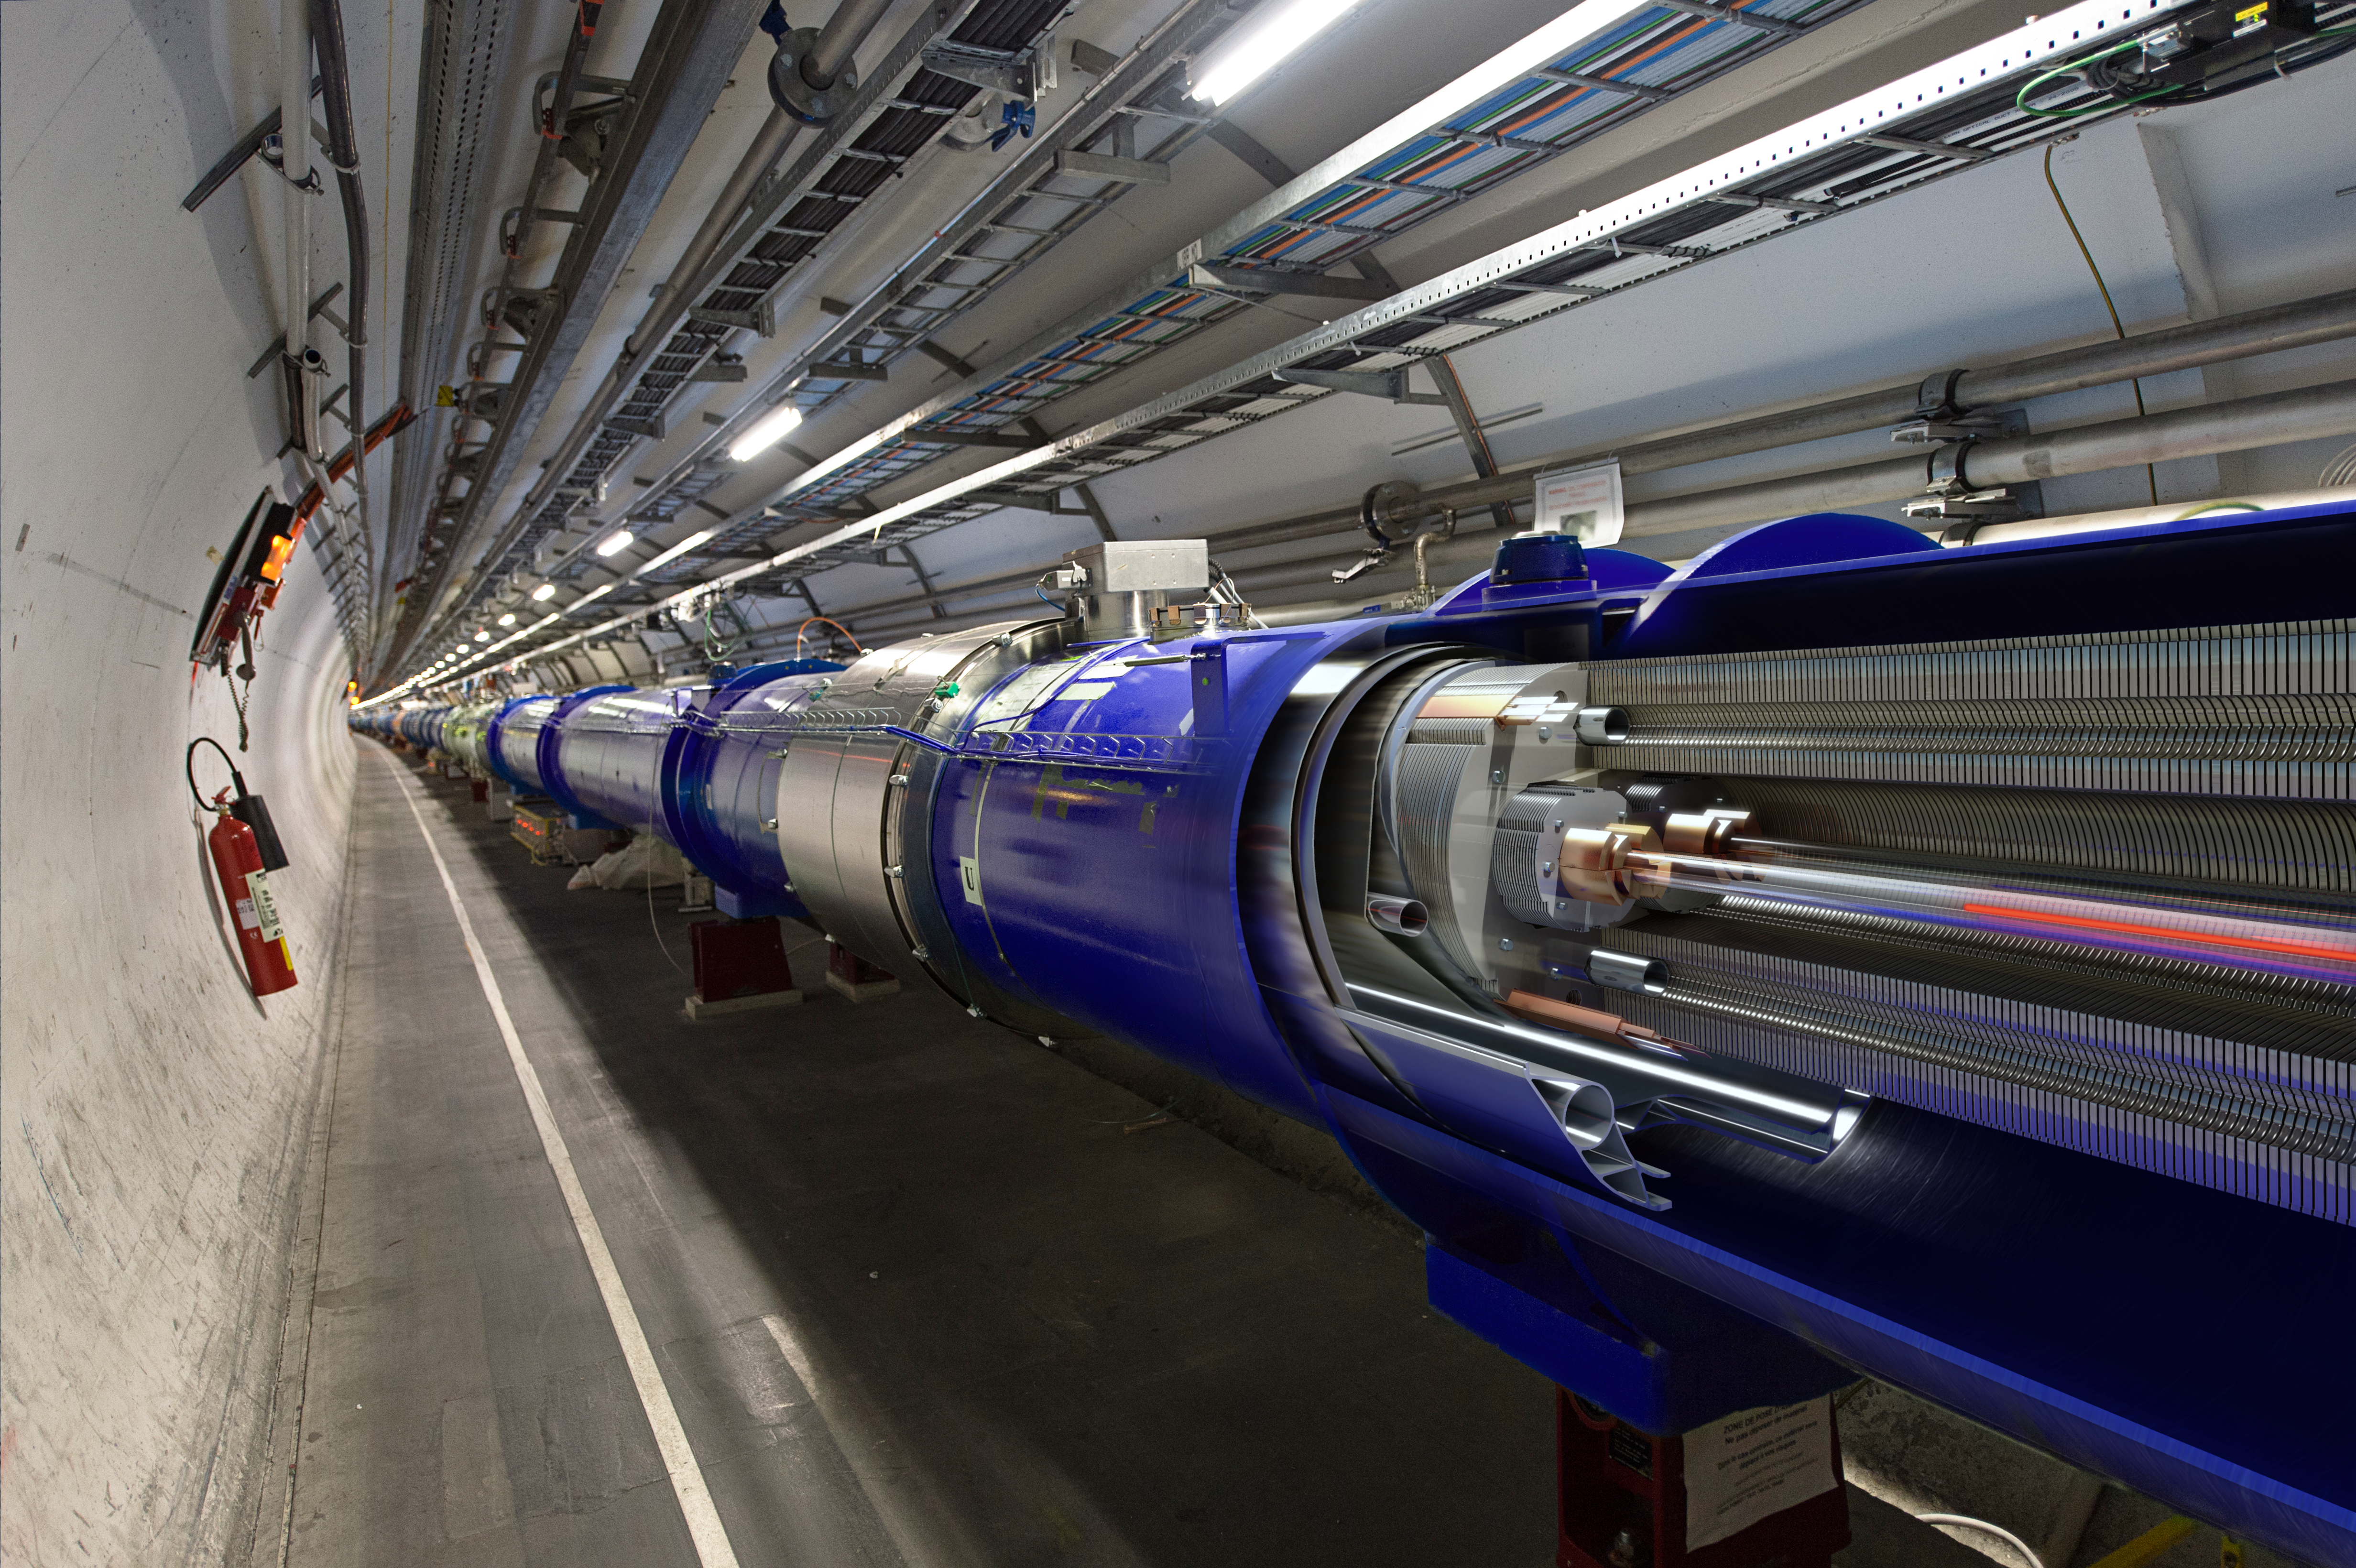
\includegraphics[width=0.8\textwidth]{chapters/01_Introduction/images/lhc_3D_cut.png}
    \caption{3D cut of a main LHC dipole~\cite{noauthor_cern_nodate}. Both beam pipes can be seen
    surrounded by the coils, strongly clamped by the yokes.}
    \label{fig:3d_cut_dipole}
\end{figure}


% -------------------------------
%   Straight Sections and Arcs
\subsubsection{\mread{Straight Sections and Arcs}}

The LHC is not a perfect circle. It is indeed composed of eight \textit{straight} sections, called
the \textit{Insertion Regions} (IRs) where detectors or specific instrumentation are placed.
Connecting those sections, the \textit{arcs} are where the majority of the magnets and their
correctors are located, along with some instrumentation like beam position monitors.
\Cref{fig:introduction:lhc_irs} shows the arcs as well as the purpose of each straight section.

\begin{figure}[!htb]
    \centering
    \includegraphics[width=0.5\textwidth]{./images/irs.png}
    \caption{Schematic of the LHC layout.}
    \label{fig:introduction:lhc_irs}
\end{figure}


% -------------------------------
%          Arc Cells
\subsubsection{\mread{Arc Cells}}

Each arc is made up of 23 cells. Magnets are organized in a standard FODO structure
(see \cref{section:courant_snyder}), as shown in \cref{fig:introduction:lhc_arc_cell}.
\textit{Dipoles} are responsible for bending the trajectory of the particles. Their associated
correctors, the orbit correctors, mitigate any possible drift in the path.
\textit{Quadrupoles} are used to control the beam size along the ring. Their effect is focusing in
one plane and defocusing in the other. Their associated correctors control the frequency of
oscillations of the beam (see tune, \cref{section:courant_snyder}) and possible field imperfections.
\textit{Sextupoles} correct chromaticity, a misfocus from quadrupoles due to particles having
a different momentum than the reference particle.
\textit{Octupoles} are used to stabilize the beam by introducing Landau
Damping~\cite{gareyte_landau_1997}. The associated correctors correct higher-order chromaticity
effects as well as amplitude-dependant tune shifts.
\textit{Decapoles} correctors aim at correcting an even higher chromaticity order.

\begin{figure}[H]
    \centering
    \includegraphics[width=1\textwidth]{./images/lhc_cell.png}
    \caption{Schematic of an LHC Arc cell~\cite{bruning_lhc_2004}.}
    \label{fig:introduction:lhc_arc_cell}
\end{figure}



% -------------------------------
%            Cycles
\subsubsection{\mread{Cycles}}

During the operation of the LHC, the machine goes through several states, each defined for specific 
scenarios~\cite{wenniger_lhc_2019}.

A common example is the operational cycle of the LHC, illustrated in \cref{fig:cern_complex:cycle}.
Initially, the magnets are pre-cycled~\cite{bottura_pre-cycles_2010} without any beam circulating,
to ensure a reproducible magnetic state. Their current is then increased to accept particles at the
injection energy of 450 GeV. To verify the machine's proper functioning, a probe bunch of reduced
intensity is first injected, at around $10^{10}$ particles. The number of bunches and their
intensity are then gradually increased to obtain the desired scheme needed for collisions, which
varies throughout the year based on experimental demands. The number of bunches and their intensity
can be adjusted as needed to ensure the machine's safety. A common scheme in 2024 is to inject about
2350 bunches, with around $1.5 \cdot 10^{11}$ particles in each bunch, for collisions. Optics
measurements, due to their destructive nature, typically use between one and three \textit{pilot}
bunches at a lower intensity of $10^{10}$ particles.

The current in the magnets is then increased along with adjustments in the phase and voltage of the
RF system to accelerate the particles to an energy of 6.8 TeV. During this ramp, the beam is
initially squeezed at the Interaction Points. However, further squeezing is limited by the
detectors' resolution, which is insufficient to accurately reconstruct a large number of collision
events simultaneously. Collisions then start, while levelling the $\beta^*$ at the ATLAS and CMS
experiments relative to the remaining beam intensity, ensuring optimal performance of the detectors.

\begin{figure}[!htb]
    \includegraphics[width=\textwidth]{./images/lhc_cycle.pdf}
    \caption{Simplified illustration of a standard LHC cycle. Adapted
    from~\cite{felix_soubelet_local_2023}.}
    \label{fig:cern_complex:cycle}
\end{figure}

\section{Magnetic Fields}

% ============================================
%                Nomenclature
% ============================================
\subsection{\review{Nomenclature}}

Several notations coexist to denote magnetic fields. In this thesis, the
\textit{European Convention}~\cite{dilly_corrections_2022} is used for field indices, as shown
in Tab.~\ref{tab:magnetic_fields:relation_indices}. MAD-X, and MAD-NG, however, use the
\textit{American Convention}.

\begin{table}[H]
    \centering
    \begin{tabular}{l|c|c|c}
        Multipole     &      MAD-X        &     Index        & Normalized Strength \\
    \hline            
        Dipole        &     0             &     1            & $K_1$   \\       
        Quadrupole    &     1             &     2            & $K_2 $  \\
        Sextupole     &     2             &     3            & $K_3 $  \\
        Octupole      &     3             &     4            & $K_4 $  \\
        Decapole      &     4             &     5            & $K_5 $  \\
        Dodecapole    &     5             &     6            & $K_6 $  \\
        Decatetrapole &     6             &     7            & $K_7 $  \\
    \end{tabular}
    \caption{Relation between field indices and multipoles.}
    \label{tab:magnetic_fields:relation_indices}
\end{table}

As such, unless explicitly stated, quantities such as the magnetic strength $b$ and normalized
strength $K$ will be expressed with this notation. 


% ============================================
%              Multipole Expansion
% ============================================
\subsection{\review{Multipole Expansion}}

A 2 dimension magnetic field in the planes \textit{x} and \textit{y} can be described as a sum of
the normal and skew field gradients $\mathcal{B}$ and $\mathcal{A}$ with multipoles of order $n$,
given by~\cite{wolf_engineering_2001}:
\begin{equation}
    B_y + iB_x = \sum_{n=1}^\infty \left(\mathcal{B}_n + i\mathcal{A}_n \right)  (x+iy)^{n-1}
\end{equation}

An ideal magnet would produce either a sole normal or skew field. However, this is not applicable 
to real-life magnets that are imperfect, due to design and manufacturing constraints.
Field errors are thus introduced, relative to the main field of the ideal 2N-pole magnet at a
reference radius $r_{ref}$~\cite{dilly_corrections_2022}, as shown in 
Eq.~\eqref{eq:magnetic_field:relative_errors}. The coefficients of the normal and skew relative 
field errors, referred to as $a_n$ and $b_n$, are dimensionless but often given in \textit{units}
of $10^{-4}$.

\begin{equation}
    B_y + iB_x = 
        \begin{cases}
            \mathcal{B}_N \cdot \sum_{n+1}^\infty (b_n + ia_n) \left(\frac{x+iy}{r_{ref}}\right)^{n-1}\text{, for normal magnets}\\
            \mathcal{A}_N \cdot \sum_{n+1}^\infty (b_n + ia_n) \left(\frac{x+iy}{r_{ref}}\right)^{n-1}\text{, for skew magnets}
        \end{cases}
    \label{eq:magnetic_field:relative_errors}
\end{equation}


The normal and skew field components of order $n$ for an imperfect 2N-pole magnet is thus given by
the following equation:

\begin{equation}
    \begin{aligned}
        \mathcal{B}_n &= \mathcal{B}_N \cdot \frac{b_n}{r_{ref}^{n-1}}, \\
        \mathcal{A}_n &= \mathcal{A}_N \cdot \frac{a_n}{r_{ref}^{n-1}}.
    \end{aligned}
\end{equation}

The unit of the field is relative to the multipole order $n$: $[\text{Tm}^{1-n}]$.


% ============================================
%              Normalization
% ============================================
\subsection{\review{Beam Rigidity and Normalization}}

\subsubsection{\review{Beam Rigidity}}

The beam rigidity refers to the resistance of a particle moving through the accelerator to the
bending applied by the magnetic fields. It is derived from the Laurentz force~\cite{dilly_corrections_2022}
and relates the magnetic field $B$, the radius of curvature $\rho$ to the momentum $p$ and charge $q$
of the particle:

\begin{equation}
    B \rho = \frac{p}{q}
    \label{eq:magnetic_fields_beam_rigidity}
\end{equation}

It is of interest when designing an accelerator to set the maximum field as well as the required
radius of curvature for a specific momentum and particle.
An interesting metric of an accelerator is also its \textit{filling factor}, or percentage of
dipoles in the machine. It can be calculated via the radius of curvature: $f = \rho / r$. A low 
filling factors means more space for other magnets, collimators, beam instrumentation, etc.

\subsubsection{\review{Field Normalization}}

The Beam Rigidity is also used as a way to normalize magnetic field strengths in particle
accelerators where the momentum of the particle changes (i.e. acceleration).
Normalized Normal and Skew components $K_n$ and $J_n$ are given by~\cite{wolf_engineering_2001}:

\begin{equation}
    \begin{aligned}
        K_n =  \frac{q}{p} &(n-1)! \mathcal{B}_n, \\ 
        J_n =  \frac{q}{p} &(n-1)! \mathcal{A}_n.
    \end{aligned}
    \label{eq:magnetic_fields_normalized}
\end{equation}



% ============================================
%            Hamiltonian Dynamics
% ============================================
\subsection{Hamiltonian Dynamics}

\todo{link to lie algebra\\
poisson bracket is a link between hamiltonian and coordinate evolutions \\
Lie Algebra uses poisson brackets}

The Hamiltonian describing the motion for the transverse planes of a given multipole or order $n$ is
given by~\cite{keintzel_jacqueline_beam_nodate,tomas_direct_2003,franchi_studies_2006}:

\begin{equation}
    \begin{aligned}
        H &= \frac{q}{p} \Re \left[ \sum_{n>1} (\mathcal{B}_n + i\mathcal{A}_n) \frac{(x+iy)^n}{n} \right] \\
          &= \Re \left[ \sum_{n>1} (K_n + iJ_n) \frac{(x+iy)^n}{n!} \right].
    \end{aligned}
    \label{eq:hamiltonian_magnet}
\end{equation}

Quite often, when studying the effect of a magnet on the beam, only one component is required, and
the sum can thus be dropped.
The normal and skew fields can also be isolated in order to consider their effect only:

\begin{equation}
    \begin{aligned}
        N_n &= \frac{1}{n!} K_n \Re \left[ (x+iy)^n \right] \\
        S_n &= -\frac{1}{n!} J_n \Im \left[ (x+iy)^n \right].
    \end{aligned}
    \label{eq:normal_skew_hamiltonian_magnet}
\end{equation}




\section{Coordinate Systems}

In circular accelerators, particle dynamics are represented using a traveling coordinate system.
A reference orbit is determined by the lattice and its magnet strengths, forming the
\textit{optics}. In the case of a synchrotron, like the LHC, where the particles return to their
original location after some turns, the reference orbit is also called the closed orbit.  
The Frenet-Serret coordinate system is used, moving along the ring on the reference orbit. The
coordinates are then transverse: $x$ and $y$, and longitudinal in the direction of travel: $s$.
Figure~\ref{fig:coordinate_systems:frenet_serret} shows those coordinates.

\begin{figure}[H]
    \centering
    \includegraphics[width=0.6\textwidth]{example-image-a}
    \caption{\todo{Frenet-Serret coordinates commonly used in accelerator physics.}}
    \label{fig:coordinate_systems:frenet_serret}
\end{figure}



% ============================================
%               Linear Lattice 
% ============================================
\subsection{Linear Lattice}

A circular accelerator is composed of many multipoles of different orders. A basic
design only requires dipoles and quadrupoles in order to operate. Dipoles are used to bend the
particles in order to form the ring, whereas quadrupoles are used to focus the beam to a focal
point, similar to light optics.
Those elements can be arranged in a particular order, to form a \text{FODO} cell. Such cells present
an alternating placement of focusing an defocusing quadrupoles with dipoles in between, as shown in
Fig.\ref{fig:coordinate_systems:fodo}, and are usually repeated many times along the ring.

\begin{figure}[H]
    \centering
    \includegraphics[width=0.6\textwidth]{example-image-a}
    \caption{\todo{FODO cell, a repeated basic block present in most circular accelerators.}}
    \label{fig:coordinate_systems:fodo}
\end{figure}

A lattice composed on of only dipoles and quadrupoles, is referred to as a \textit{linear} lattice.

\todo{
    Courant Snyder/Twiss
    Tune, beta function
% 
    Lie, normal form
    Resonance Driving Terms
}
\section{Beam Observables}

\todo{title?\\
Linear observables\\
Optics}

% ============================================
%               Dispersion
% ============================================
\subsection{\review{Dispersion}}

Treating a beam as a single particle having the design momentum $p_0$ leads to a machine with no
apparent ill effect related to that momentum.
However, when considering a particle beam where each particle follows a distribution in
momentum, a few effects arise from this deviation, called the \textit{momentum offset},
$\delta$. It is defined as a relative difference to the design momentum:

\begin{equation}
    \delta = \frac{p - p_0}{p_0}.
    \label{eq:coordinate_systems:momentum_offset}
\end{equation}

Those effects are referred to as \textit{chromatic aberrations}. The first and most important to
consider is the \textit{dispersion}. Dispersion results from a particle with a momentum offset
being deflected differently by the dipoles compared to a particle at the design momentum.
Figure~\ref{fig:coordinate_systems:dispersion} shows an example of deflection. 

\begin{figure}[H]
    \centering
    \includegraphics[width=0.6\textwidth]{images/dipole.pdf}
    \caption{Particles with a momentum offset will be deflected differently by dipoles. This offset
            in position can be described by the dispersion function.}
    \label{fig:coordinate_systems:dispersion}
\end{figure}

The particle is still subject to the other properties of the lattice, but with a different orbit,
described by Eq.~\eqref{fig:coordinate_systems:dispersion}.

\begin{equation}
    \begin{aligned}
    D_x(s) = \frac{\Delta x(s)}{\delta} \\
    D_y(s) = \frac{\Delta y(s)}{\delta} \\
    \end{aligned}
    \label{eq:coordinate_systems:dispersion}
\end{equation}



% ============================================
%               Beta Function
% ============================================
\subsection{\todo{$\beta$-function}}

As seen previously in~\ref{section:courant_snyder}, the $\beta$-function is related to the amplitude
of oscillations of the beam. Figure~\ref{fig:beam_optics:beta} shows how the $\beta$-function
oscillates along the ring due to quadrupoles focusing and defocusing properties.
The $\beta$-function is an important quantity found as a factor in several other observables that
will be described later in this thesis.


\begin{figure}[H]
    \centering
    \includegraphics[width=0.9\textwidth]{images/beta_function.pdf}
    \caption{Evolution of the $\beta$-function along the lattice. Horizontal and vertical beatings
    are usually opposite given the focusing and defocusing properties of quadrupoles in each plane.}
    \label{fig:beam_optics:beta}
\end{figure}

A difference in $\beta$-function compared to the design leads to possible unstable and larger beams,
degrading its properties and making it harder to control. The relative difference in
$\beta$-function is called the beta-beating, expressed in percents: 

\begin{equation}
    \mathrm{beating \; [\%]}  = \frac{\beta_z(s) - \beta_z(s)_{model}}{\beta_z(s)_{model}}.
    \label{eq:beam_optics:beating}
\end{equation}


% ============================================
%                  Coupling
% ============================================
\subsection{\review{Coupling}}

In a perfect scenario, the particle motion of each transverse plane is independent, or
\textit{uncoupled}. In practice, this transverse motion can be altered by some magnetic elements,
giving rise to \textit{betatron coupling} where the motion of each plane is not independent anymore.
Such elements can be quadrupoles, mounted with a roll error introducing skew-quadrupolar fields,
which are the main source of coupling in the LHC~\cite{felix_soubelet_local_2023}. Field
imperfections, solenoids and feed-down from higher orders can also contribute to coupling.

The resonances $Q_x + Q_y$ and $Q_x - Q_y$, called the \textit{sum} and \textit{difference}
resonances, are mainly excited by skew quadrupoles. When coupling is present in the
machine, the former may lead to unstable motion while the latter introduces an periodic exchange of
emittance between the planes, keeping it stable. They can be characterized by the RDTs $f_{1010}$
and $f_{1001}$.

Effects of normal multipoles start showing their skew counterpart (and vice versa) as the motion
of transverse planes become coupled. This is demonstrated in \cref{chapter:skew_octupole_fields}
with skew-octupolar RDTs contributed to by normal octupoles in the presence of coupling.


% ============================================
%         Momentum Compaction Factor
% ============================================
\subsection{\todo{Momentum Compaction Factor}}
\label{subsection:coordinates_systems:momentum_compaction_factor}

In synchrotrons, particles with a deviation in momentum with respect to the reference particle will
experience a different path length due to the bending of the dipoles. This effect is characterized
by the \textit{momentum compaction factor}~\cite{keintzel_jacqueline_beam_nodate},

\begin{equation}
    \alpha_c = \frac{\Delta C / C}{\delta},
\end{equation}

relating the circumference of the ring $C$ to the momentum offset $\delta$.
A positive momentum compaction factor indicates a longer path traveled by particles with a positive
momentum offset, and vice versa.


The momentum compaction factor can also be broken down into orders as an infinite sum, where the
linear term is often referred to as the first order,

\begin{equation}
    \alpha_c = \underbrace{\alpha_{c,0}}_{\text{Linear term}}
               + \underbrace{\sum_{i \geq 1} \alpha_{c, i} \delta^i}_\text{Non linear terms}.
\end{equation}

In the LHC, the contribution from the non linear terms is
negligible~\cite{keintzel_jacqueline_beam_nodate}. Further details can be found
in~\cref{subsection:decapoles:chromaticity:measurement}.
\section{Detuning Effects}


% ============================================
%                Chromaticity
% ============================================
\subsection{\review{Chromaticity}}

Chromaticity is the tune change $\Delta Q$ relative to the momentum offset $\delta$. Chromaticity
can be described by a Taylor expansion, given by

\begin{equation} 
    Q (\delta) = Q_0 + Q' \delta + \frac{1}{2!} Q'' \delta^2 + \frac{1}{3!} Q''' \delta^3 + \mathcal{O}(\delta^4).
    \label{eq:background_chromaticity}
\end{equation}

Or, more generally, rewritten as a sum to include all orders up to $n$:

\begin{equation}
    Q (\delta) = Q_0 + \sum_{i=1}^n \frac{1}{i!} Q^{(i)} \delta^i.
    \label{eq:background_chromaticity_sum}
\end{equation}


The first order of the chromaticity expansion, $Q'$, is generally simply referred to as 
\textit{chromaticity}, sometimes as \textit{linear chromaticity}.
The other terms are thus referred to as \textit{non-linear chromaticity}.

The chromaticity change induced by a single element of order $n$ and length $L$ can be derived from
the Hamiltonian of Eq.~\eqref{eq:hamiltonian_magnet}, averaging over the phase variables and
differentiating relative to the actions $J_{x,y}$ and the momentum offset $\delta$:

\begin{equation}
    \Delta Q^{(n)}_{x,y} = \frac{\partial^n Q_{x,y}}{\partial^n \delta} = 
      \frac{1}{2\pi} \int_L \left< \frac{\partial^{(n+1)} H}{\partial J_{x,y}\partial^n \delta}\right> \diff s.
    \label{eq:background_chroma_order_hamiltonian}
\end{equation}


% =========
\subsubsection{Natural Chromaticity from Quadrupoles}

In a purely linear lattice, the linear chromaticity, $Q'$, is a result of the momentum dependence 
of the quadrupoles' focusing. It is in this case called the \textit{natural chromaticity} and can be
derived from the normal hamiltonian of Eq.\eqref{eq:normal_skew_hamiltonian_magnet} and expressing
the normalized magnet strength $K$ with a dependence on $\delta$ via $P$ as $P_0(1+\delta)$:

\begin{equation}
    K_n = \frac{q}{P_0} \frac{1}{1 + \delta} (n - 1)! B_n
    \label{eq:k_dpp}
\end{equation}

The normal field of a quadrupole is then given by

\begin{equation}
    \mathcal{N}_2(x,y) = \frac{1}{2} \frac{q}{P_0} \frac{1}{1+\delta} B_2 (x^2 - y^2)
\end{equation}

By operating a variable change to the angle coordinates 
(\(x \rightarrow \sqrt{2 J_x \beta_x} \cos \phi_x\) and
\(y \rightarrow \sqrt{2 J_y \beta_y} \cos \phi_y\)), the following equation linking the $\beta$-function
and $\delta$ to the normal field is obtained:
\begin{equation}\mathcal{N}_2 (x,y) = \frac{1}{2} \frac{q}{P_0} \frac{1}{1+\delta} B_2 
        \left[
            \left(\sqrt{2 J_x \beta_x} \cos \phi_x \right)^2 
            - \left(\sqrt{2 J_y \beta_y} \cos \phi_y\right)^2
        \right].
    \label{eq:hamiltonian_quadrupole_angle}
\end{equation}

Following Eq.\eqref{eq:background_chroma_order_hamiltonian}, the natural chromaticity $Q'$ induced by
quadrupoles is given by:
\begin{equation}
    \begin{aligned}
        \Delta Q'_x &= \frac{1}{2\pi} \int_L \frac{\partial^2 \left< \mathcal{N}_2 \right> }{\partial J_x \partial \delta} \diff s
        \quad;\quad
        \Delta Q'_y &= \frac{1}{2\pi} \int_L \frac{\partial^2 \left< \mathcal{N}_2 \right>}{\partial J_y \partial \delta} \diff s
        \\
        & = - \frac{1}{4 \pi} \frac{q}{P_0} B_2 L \beta_x
        & = \frac{1}{4 \pi} \frac{q}{P_0} B_2 L \beta_y
    \end{aligned}
\end{equation}


% =========
\subsubsection{Linear Chromaticity from Sextupoles}

The first order chromaticity $Q'$ is contributed to by sextupoles in the presence of off-momentum
particles. The normal field of a sextupole, following Eq.\eqref{eq:normal_skew_hamiltonian_magnet}
is given by

\begin{equation}
    \mathcal{N}_3(x,y) = \frac{1}{3!} (x^3 - 3xy^2).
    \label{eq:detuning:linear_chromaticity}
\end{equation}

As the momentum offset $\delta$ introduces a change in orbit via
dispersion~\cite{keintzel_second-order_2019}, a variable change can be operated on both $x$ and $y$,
as shown in Eq.\eqref{eq:detuning:offset}. In this thesis, vertical dispersion will be though
neglected.

\begin{equation}
    \begin{aligned}
        x &\rightarrow x + \Delta x = x + D_x\delta \\
        y &\rightarrow y + \Delta y = y + D_y\delta
    \end{aligned}
    \label{eq:detuning:offset}
\end{equation}

The positions $x$ and $y$ can once be replaced, using the twiss parameters, giving the full
expression:

\begin{equation}\begin{aligned}
  \mathcal{N}_3(x + \Delta x, y) = \frac{1}{6} K_3 \biggl[&
       \left(\sqrt{2 J_x \beta_x} \cos \phi_x\right)^3 \\
  &    + 3 \left(\sqrt{2 J_x \beta_x} \cos \phi_x\right)^2 D_x \delta \\
  &    + 3 \left(\sqrt{2 J_x \beta_x} \cos \phi_x\right) D_x^2 \delta^2 \\
  &    + D_x^3 \delta^3 \\
  &    - 3 \left(\sqrt{2 J_x \beta_x} \cos \phi_x \right) \left(\sqrt{2 J_y \beta_y} \cos \phi_y \right)^2 \\
  &    - 3 D_x \delta (\sqrt{2 J_y \beta_y} \cos \phi_y)^2 \biggl]
\end{aligned}\end{equation}

Averaging over the phase variables removes any odd cosine:
\begin{equation}\begin{aligned}
  \left< \mathcal{N}_3(x + \Delta x, y) \right> = \frac{1}{6} K_3 &\biggl(
       3 J_x \beta_x D_x \delta \\
  &    + D_x^3 \delta^3 \\
  &    - 3 D_x \delta J_y \beta_y \biggl)
\end{aligned}\end{equation}



The chromaticity can then obtained by differentiating relative to the action $J_{x,y}$ to obtain the
tune, and then by the momentum offset $\delta$.
\begin{equation}
    \begin{aligned}
        \Delta Q'_x &= \frac{1}{2\pi} \int_L \frac{\partial^2 \left< \mathcal{N}_3 \right>}{\partial J_x \partial \delta} \diff s \quad; \quad \Delta Q'_y &&= \frac{1}{2\pi} \int_L \frac{\partial^2 \left< \mathcal{N}_3 \right>}{\partial J_y \partial \delta} \diff s \\
        &= \frac{1}{2 \pi} L \frac{1}{2} K_3 \beta_x D_x  &&= - \frac{1}{2 \pi} L \frac{1}{2} K_3 \beta_y D_x \\
        &= \frac{1}{4 \pi}  K_3 L \beta_x D_x &&= - \frac{1}{4 \pi}  K_3 L \beta_y D_x
    \end{aligned}
\end{equation}

From this last equation, it is apparent than sextupoles are not a source of chromaticity of higher
orders in the presence of linear dispersion. In the presence of second order
dispersion~\cite{keintzel_second-order_2019}, sextupoles can generate some amount of $Q''$, usually
negligible.


% =========
\subsubsection{Non-Linear Chromaticity}

Higher orders of the chromaticity function are described in~\cite{dilly_derivation_2023} and follow
the same logic as for the linear chromaticity from sextupoles.





% ============================================
%             Amplitude Detuning
% ============================================
\subsection{Amplitude Detuning}



% ============================================
%        Chromatic Amplitude Detuning
% ============================================
\subsection{Chromatic Amplitude Detuning}

\todo{make it clear I derived it}
\section{Resonances}


%----------------------------------------
%
%----------------------------------------

\begin{figure}[H]
    \centering
    \includegraphics[width=0.7\textwidth]{images/resonance_diagaram_n5.png}
    \caption{Tune diagram with resonances lines excited by multipoles up to decapole ($n \leq 5$).
             The working point of the machine is chosen in an area where few lines are present.}
    \label{fig:resonances:diagram_n5}
\end{figure}


\begin{figure}[H]
    \centering
    \includegraphics[width=0.7\textwidth]{images/resonance_diagaram_n7.png}
    \caption{Tune diagram with resonances lines excited by multipoles up to decatetrapole 
             ($n \leq 7$). When considering higher orders, it becomes apparent that the beam will
             hit several resonances.}
    \label{fig:resonances:diagram_n7}
\end{figure}

% ----------------------------------
% Optics Measurements and Correction
% ----------------------------------
\chapter{\review{Optics Measurements and Corrections}}
\label{chapter:optics_meas}
\section{\review{Beam Instrumentation}}


% ============================================
%          Beam Position Monitors
% ============================================
\subsection{\review{Beam Position Monitors}}

Beam Position Monitors (BPMs) are one of the most utilized and essential elements of beam 
diagnostics in particle accelerators. In the LHC, most of the BPMs are dual plane, and thus composed
of four electrodes, distributed as two per plane. The BPM system consists of over than 550 BPMs pear
beam, positioned along the ring, in the arcs and the IPs. The most common type, the
\textit{curved-button}, shown in \cref{fig:beam_instrumentation_bpm_button}, is typically placed
near quadrupoles~\cite{wendt_bpm_2020}.

\begin{figure}[H]
    \centering
    \begin{subfigure}[b]{0.45\textwidth}
        \includegraphics[width=\textwidth]{images/lhc_bpm_button.jpg}
        \caption{Button \textit{"BPM"} type BPM of the LHC~\cite{wendt_bpm_2020}.}
        \label{fig:beam_instrumentation_bpm_button}
    \end{subfigure}
    \hfill
    \begin{subfigure}[b]{0.45\textwidth}
        \includegraphics[width=\textwidth]{images/lhc_bpm_stripline.jpg}
        \caption{Stripline \textit{"BPMSW"} type BPM of the LHC~\cite{wendt_bpm_2020}.}
        \label{fig:beam_instrumentation_bpm_stripline}
    \end{subfigure}
\end{figure}

Other pickups such as the \textit{stripline}, shown in
\cref{fig:beam_instrumentation_bpm_stripline}, albeit more complex and expensive, offer a better
signal to noise ratio and are capable of identifying the direction of the
beam~\cite{wendt_bpm_2020}. Such features are essential for the LHC, were both beams travel through
the same aperture at the IPs.\\ 
%The BPM response is not linear with the beam position, which requires a post-processing not
%systematically implemented in accelerators beam diagnostics systems. LHC's BPMs have been simulated
%and polynomials fitted to minimize this response error~\cite{a_nosych_geometrical_2014}.


 
% ============================================
%                Collimators
% ============================================
\subsection{\review{Collimators}}

Collimators are a crucial part of the LHC. Their purpose is to protect the machine against beam
losses and clean the outer parts of the beam~\cite{redaelli_lhc_2011}. The energy of the beams in
the LHC is high enough to not only quench the magnets, but to also damage the elements.

At injection energy, with a low intensity pilot bunch, the consequences of a loss are though less
severe. During Run 3, in 2022, a new collimator sequence was introduced, making a safe exploitation
of the machine possible with more retracted collimators. This made measurements with higher kick
amplitudes and larger orbit offsets, and thus momentum offsets, possible.


% ============================================
%             Beam Loss Monitors
% ============================================
\subsection{\review{Beam Loss Monitors}}

Beam Loss Monitors are detectors mounted on various elements of the accelerator, such as magnets or
collimators, to detect abnormal losses of particles. They play a crucial role in the protection of
the machine, triggering a dump when losses exceed the threshold set for their respective element. 
BLMs use ionization chambers, working on the same principle as simple Geiger counters: a tube filled
with gas, in presence of a high voltage~\cite{schmidt_machine_2014}. A picture of BLMs mounted on
the LHC is given in \cref{fig:beam_instrumentation:blm1}.

Dashboards in the control room are regularly used to monitor the losses along the ring when
performing optics measurements, as those prove to often be destructive. An example of such a
dashboard is given in \cref{fig:beam_instrumentation:blm2}.

\begin{figure}[H]
    \centering
    \includegraphics[width=0.6\textwidth]{images/blm.png}
    \caption{Beam Loss Monitors (BLM), in yellow, on the LHC~\cite{schmidt_machine_2014}.}
    \label{fig:beam_instrumentation:blm1}
\end{figure}

\begin{figure}[H]
    \centering
    \includegraphics[width=0.6\textwidth]{images/blm2.png}
    \caption{Graphical interface used in the CERN Control Cernter (CCC) for instantaneous losses in
    the LHC~\cite{schmidt_machine_2014}. Different parts of the accelerator have varying dump
    thresholds.}
    \label{fig:beam_instrumentation:blm2}
\end{figure}


% ============================================
%                   BCT
% ============================================
\subsection{\review{Beam Current Transformer}}

The Beam Current Transformer (BCT) is a device used to measure the intensity of a particle beam.
It operates by detecting the current induced by the moving charge of the beam as it passes through
the tores of the BCT.
The BCTs are designed to be able to measure intensities from pilots bunches of 8µA to total beams of
more than 860mA~\cite{odier_dcct_2009}.


% ============================================
%                   BBQ
% ============================================
\subsection{\review{BBQ System}}

The Base-Band Tune (BBQ) system in the LHC is designed to measure the beam's tune via its
turn-by-turn signal. It operates by detecting and analyzing the signals of diode
peak-detectors~\cite{boccardi_first_2009}. The system further implements processing hardware and
software, transmitting the acquired data to the control and logging systems.
The system can operate with no explicit excitation, relying on the residual beam
oscillations, or by using tune kickers or frequency sweeps~\cite{boccardi_first_2009}.


% ============================================
%                 AC-Dipole
% ============================================
\subsection{\review{AC-Dipole}}

The AC dipole of the LHC is a crucial component for optics studies. Its primary function is to
excite the beam into large coherent oscillation, achieved by applying a sinusoidally oscillating
dipole field~\cite{miyamoto_parametrization_2008}. By ramping up and down adiabatically the field,
large coherent oscillations can be produced without any decoherence or emittance growth.
\Cref{fig:ac_dipole} shows an example of a simulation made with an AC-Dipole. Exciting the beam to
large amplitudes make the study of linear optics, such as beta-beating easier, and that of non
linear optics such as resonances possible.

\begin{figure}
    \center
    \includegraphics[width=0.85\textwidth]{./images/ac_dipole_tbt.pdf}
    \caption{Simulated turn by turn data with an AC-Dipole first ramping up then down.} 
    \label{fig:ac_dipole}
\end{figure}

The AC-Dipole is set to oscillate at a frequency $Q_d$, different from the natural tune of the
machine $Q$ and thus introduces systematic effects that needs to be compensated during the optics
analysis. The new orbit of a particle under the influence of the AC-Dipole, at turn number $n$ and
observation point $s$, is given by~\cite{serrano_lhc_2010}:

\begin{equation}
z(s, n) = \frac{BL}{4\pi\rho\delta_z} \cdot \sqrt{\beta_z(s) \beta_{z,0}} \cdot \cos \left( 2 \pi Q_{d,z}n + \phi_z(s) + \phi_{z,0}\right),
\label{eq:ac_dipole}
\end{equation}

where $B$ is the amplitude of the oscillating magnetic field, $L$ the length of the AC-Dipole,
$B\rho$ the magnetic rigidity, $\delta$ the difference between $Q_d$ and $Q$, $\beta$ and $\beta_0$
the beta function at the observed point and the AC-Dipole, $\phi$ and $\phi_0$ the phase advance at
the observed point and of the AC-Dipole.
\section{\review{Optics Measurements}}

To perform optics measurements, several tools and techniques are used. This section details the
various implemented methods to measure specific observables.

% ===============================
%            Software
% ===============================
\subsection{\review{Tools and Softwares}}

In order to perform the measurements, analysis and simulations presented in this thesis, various
tools and softwares have been developed, used and contributed to.

Optics simulations have been done mainly in MAD-X~\cite{deniau_mad-x_nodate} and PTC.
MAD-NG~\cite{deniau_mad-ng_2020} and
Xsuite~\cite{g_iadarola_xsuite_nodate} have also been explored for specific tasks such as free RDT
simulations and GPU tracking.

Analysis of chromaticity measurements are done via a newly developed graphical
interface~\cite{m_le_garrec_non-linear_2022} written in Python. This tool makes cleaning of the raw
signal data, its analysis and results export more reliable and easier.

Overall, analysis of turn-by-turn measurements is supported by a large panel of libraries written by
the OMC team in Python and Java. Contributions have mainly been made to extend the following
packages:


\begin{itemize}
    \item \textbf{Beta-Beat GUI}~\cite{omc-team_beta-beat_2008}, Graphical interface for
    turn-by-turn measurements visualization and analysis.
    \item \textbf{OMC3}~\cite{omc-team_omc3_2021}, Main optics analysis and corrections software.
    \item \textbf{Beta-Beat.src}~\cite{omc-team_beta-beatsrc_2018}, Old analysis software, now
    replaced by OMC3.
    \item \textbf{pylhc.github.io}~\cite{omc-team_omc_2020}, Website of the OMC team with package
    documentation, examples and useful resources.
\end{itemize}


% ===============================
%           TbT Data
% ===============================
\subsection{\review{Turn-by-Turn Signal}}

One of the key data acquisition methods for optics measurements in the LHC is turn-by-turn
acquisition, where beam position is collected on a per-turn basis. This process involves exciting
the beam using an AC-Dipole to induce forced oscillations. Typically, a pilot bunch is used for
this purpose, containing a reduced intensity of $10^{10}$ protons, compared to the standard
operational bunch intensity of $10^{11}$. The lower intensity allows for larger amplitude
oscillations, enabling more precise measurements while ensuring the safety of the machine and
minimizing the risk of damaging components.

A spectral analysis is then performed via a \textit{FFT} on the signal, making apparent the driven
tunes from the AC-Dipole, the transverse tunes and the possible resonance lines, as shown in
\cref{fig:optics_measurements:tbt_data:spectrum}.

\begin{figure}[!htb]
    \centering
    \includegraphics[width=0.8\textwidth]{./images/basic_spectrum.pdf}
    \caption{Horizontal frequency spectrum of a turn-by-turn measurement in the LHC. The 
    \textit{driven} tunes of the AC-Dipoles have the highest amplitudes while the natural tune can
    be seen close to it. Other lines are often created by resonances.}
    \label{fig:optics_measurements:tbt_data:spectrum}
\end{figure}

From these oscillations and  spectral lines, the optics observables, such as $\beta$-beating,
dispersion, coupling, and resonance driving terms, can be
reconstructed~\cite{catalan-lasheras_linear_2004}. These key quantities provide valuable insights
into the beam's dynamics and will be detailed further in the following sections.

\FloatBarrier

% ------- Betatron Phase
\paragraph{\review{Betatron Phase}}
The betatron phase can be determined at a given BPM by performing an FFT on the turn-by-turn
data. The angle of the main peak, the tune, is then taken to obtain the phase. The phase advance
between two BPMs is simply their phase difference.


% ------- Beta Beating
\paragraph{\review{$\beta$-Beating}} 
The $\beta$-beating can be reconstructed via the phase advance between BPMs. The computation
involves using a model created via a simulation software such as MAD-X. The $beta$-function at a
given BPM can be calculated from the measured phases of 3 BPMs denoted $i, j,
k$~\cite{minty_measurement_2003},

\begin{equation}
    \beta(s_i) = \beta^{model}(s_i) \cdot \frac{\cot(\Delta\phi_{i,j}) + \cot(\Delta\phi_{i,k})}{\cot\left(\Delta\phi_{i,j}^{model}\right) + \cot\left(\Delta\phi_{i, k}^{model}\right)}
\end{equation}

with $\Delta_{i,j}$ being the phase advance between BPMs $i$ and $j$. Using specific phase advances
between BPMs enhances the precision of the $\beta$-function measurement. This approach can also be
extended to use an arbitrary number $N$ of
BPMs~\cite{langner_utilizing_2016,wegscheider_analytical_2017}. The measurement of the
$\beta$-function via phase advance is independent from BPM calibration and relies solely on the
accuracy of the phase measurement.


% ------- Dispersion
\paragraph{\review{Dispersion}} To retrieve the linear dispersion, turn-by-turn measurements are
performed at certain momentum offsets. This allows the computation of the dispersion via the shift
in mean orbit $\Delta z$ and the momentum offset $\delta$,

\begin{equation}
    D_z = \frac{\Delta z}{\delta}.
\end{equation}

In the LHC, measurements are typically taken at $\pm 100$Hz, corresponding to a momentum offset 
$\delta \approx \mp0.7$.


% ------- Action
\paragraph{Action} 
The action in a given plane and BPM, located at position $s$ is calculated from the amplitude
$\mathcal{A}$ of the main peak in the frequency spectrum, which corresponds to the tune, along with
the beta-function at that BPM derived from the model,

\begin{equation}
    2J_{BPM} = \frac{\mathcal{A}_{BPM}^2}{\beta_{model,BPM}}.
\end{equation}

This method of action computation is directly influenced by BPM calibration
errors~\cite{garcia-tabares_valdivieso_optics-measurement-based_2020}. The overall action is then
the average over $n$ BPMs:

\begin{equation}
    2J = \frac{1}{n} \sum_n \frac{\mathcal{A}_n^2}{\beta_{model,n}}.
\end{equation}


% ------- Coupling
\paragraph{\review{Coupling}}

Coupling can be calculated by comparing the amplitude of the tune in the frequency spectrum of a
plane to the same tune in the other plane. The coupling RDTs $f_{1001}$ and $f_{1010}$ can be
reconstructed with these amplitudes~\cite{franchi_computation_2010,tomas_cern_2010},

\begin{equation}
    \begin{aligned}
        |f_{1001}| &= \frac{1}{2} \sqrt{\frac{H(0,1)V(1,0)}{V(0,1)H(1,0)}}, \\
        |f_{1010}| &= \frac{1}{2} \sqrt{\frac{H(0,-1)V(0,-1)}{V(0,1)H(1,0)}},
    \end{aligned}
\end{equation}

where H(1, 0) is the amplitude of $Q_x$ in the horizontal spectrum while H(0, 1) corresponds to
$Q_y$ in the same spectrum. The phases of these RDTs is given by,

\begin{equation}
    \begin{aligned}
        q_{1001} &= \phi_{V(1,0)}  - \phi_{H(1,0)} + \frac{\pi}{2}, \\
        q_{1010} &= \phi_{H(0,-1)} - \phi_{V(0,1)} + \frac{\pi}{2}.
    \end{aligned}
\end{equation}

The final expression of the coupling RDTs is then,

\begin{equation}
    \begin{aligned}
        f_{1001} &= |f_{1001}|e^{i\cdot q_{1001}},\\
        f_{1010} &= |f_{1010}|e^{i\cdot q_{1010}}.
    \end{aligned}
\end{equation}


% ------- Amplitude Detuning
\paragraph{\review{Amplitude Detuning}}
Amplitude detuning measurements in the LHC are usually taken with varying AC-Dipole kick amplitudes.
A linear function is then fitted on the natural tunes $Q_x$ and $Q_y$ versus the action of either
planes $2J_x$ or $2J_y$.


% ------- Resonance Driving Terms
\paragraph{\review{Resonance Driving Terms}}
Resonance Driving Terms are measured in the LHC with varying AC-Dipole kick amplitudes. The
amplitude of the resonance line of interest in the frequency spectrum can then be fitted to the
corresponding action dependence of the RDT, as detailed in
\cref{section:background:frequency_spectrum} and \ref{appendix:rdts}. As a reminder, the amplitude
of the RDT will be given by,

\begin{equation}
    \begin{aligned}
    |f_{jklm}| &= \frac{|H_{f_{jklm}}|}{2 j (2 I_x)^\frac{j+k-1}{2} (2 I_y)^\frac{l+m}{2}} \\
    |f_{jklm}| &= \frac{|V_{f_{jklm}}|}{2 l (2 I_x)^\frac{j+k}{2} (2 I_y)^\frac{l+m-1}{2}} .
    \end{aligned}
    \nonumber
\end{equation}

The phase of the RDT can then be reconstructed via the momentum and phase advances. In practice,
\textit{forced resonance driving terms} are actually measured, as the oscillations are driven by
the AC-Dipole. Simulations are thus always made via tracking with an AC-Dipole to match.
Studies linking \textit{forced} RDTs to \textit{free} RDTs is though ongoing to better understand
the machine without excitation~\cite{carlier_nonlinear_2020}.


% ------- Lifetime
\paragraph{\review{Lifetime}}

The beam lifetime is a measure of how long the beam can remain circulating without significant
losses of particles. It is typically expressed in hours and is related to the rate
at which particles are lost from the beam. The beam intensity is measured via the BCTs. The lifetime
$\tau$ relates then the number $N$ of particles at a time $t$ to its rate of change,

\begin{equation}
    \tau = N(t) \cdot \frac{\diff N}{\diff t}^{-1}.
\end{equation}

Additionally, Beam Loss Monitors (BLMs) provide local information about beam quality by detecting
and localizing particle losses. These losses can as well be integrated to give a lifetime estimate.
At injection energy in the LHC, the beam lifetime with a pilot bunch is typically around 3 hours.
Sudden particle losses can significantly reduce the measured lifetime, even if the remaining beam
stabilizes and does not lose particles as rapidly. This introduces challenges in accurately
measuring the lifetime, as the signal needs to stabilize and saturate after any trim to ensure
reliable data.


% ===============================
%          Chromaticity
% ===============================
\subsection{\review{Chromaticity}}
\label{subsection:optics_corrections_chromaticity}

%% --- Procedure ---
%\subsubsection{\review{Procedure}}

Contrary to the previously seen observables, chromaticity measurements are performed by varying
the RF frequency to induce a change of momentum offset $\delta$, while measuring the tune. The
momentum offset $\delta$ being related to the RF frequency, the Lorentz factor $\gamma$ and the
momentum compaction factor $\alpha_c$~\cite{keintzel_jacqueline_beam_nodate}:

\begin{equation}
    \delta = - \left(\frac{1}{\gamma^{-2} + \alpha_c}\right) \cdot \frac{\Delta f_{\text{RF}}}{f_{\text{RF,nominal}}}
    \label{eq:dpp_rf}
\end{equation}

In the LHC, the Lorentz factor $\gamma^{-2}$ is here negligible, as the energy is large even at
injection.  At 450GeV, $\gamma^{-2} \approx 10^{-6}$, which is two orders of magnitude smaller than
$\alpha_c$.

During operation, where the linear chromaticity often needs to be measured, a sinusoid function is
applied on the RF frequency. This induces a short range of momentum offset, but enough to measure
the first order of the chromaticity function.
For non-linear measurements, a larger range is required. In order to do so, a new procedure has been
developed. Dense frequency scans with steps of 20Hz every 30 seconds are usually taken to compromise
between number of data points, precision of the tune estimate, and duration of the measurement. Once
beam losses, registered by the BLMs are deemed too high, the frequency is reverted back to its
nominal value in larger steps. Attaining the limits of the BLMs ensures a large momentum-offset
range. The same procedure is then re-applied in the negative. \Cref{fig:measurements:rf_scan} shows
a typical RF scan performed to measure chromaticity in the LHC.

\begin{figure}[H]
    \centering
    \includegraphics[width=1\textwidth]{images/rf_scan.pdf}
    \caption{Observation of the tune dependence on momentum offset, created by a shift of RF
             frequency.}
    \label{fig:measurements:rf_scan}
\end{figure}


%% --- Analysis and Fit ---
%\subsubsection{\review{Analysis}}

Once the tunes have been acquired and the momentum offset computed via \cref{eq:dpp_rf}, the
chromaticity function (see \cref{eq:background_chromaticity}) can be used to fit the
measured data and retrieve each order.

As part of the work for this thesis, a new tool, was developed. in order to ease and improve the
analysis of chromaticity measurements. 
The Non-Linear Chromaticity GUI~\cite{m_le_garrec_non-linear_2022} showcases new analysis techniques
using the raw signal from the BBQ system along with custom signal cleaning that are detailed later
on in \cref{chapter:high_order_fields}. Fits to very high chromaticity orders are also now possible
along with their computed corrections and that of resonance driving terms via a combined response
matrix approach. Automatic data extraction from the CERN data servers (Timber, NXCALS) is also
included.
\section{Correction Principles}


% ===============================
%        Response Matrix
% ===============================
\subsection{\review{Response Matrix}}

A response matrix is a linear equation system that describes the change of an observable for a set
of individual multipole strengths. By taking the pseudo-inverse of this matrix and multiplying it to
the measured observables, a set of corrector strengths if obtained that can replicate the measured
value. Taking the opposite sign then gives a correction.  This technique is routinely used to
correct, amongst others, \beta-beating as well as Resonance Driving Terms. In situations where
measurements are taken at each BPM for a particular observable, the corresponding response matrix
ends up containing over 500 values per corrector, for a single beam.

Individual MAD-X simulations are run with a single multipole powered at a time. The resulting
parameter values (e.g. \beta-beating) are then compared to those obtained from a simulation without
any powering, allowing to determine the specific impact of each multipole.

A response matrix is thus created following Eq.~\eqref{eq:resp_matrix}, for a matrix of observables
$O$, a reference matrix of observables without any corrector $O_R$ and a fixed multipole strength
$k$. Given measured data $M$, the set of correctors needed to compensate the values can be obtained
by taking the pseudo-inverse of the matrix in Eq.~\eqref{eq:resp_matrix_inverted}.

\begin{equation}
  R = \left(O - O_R \right) \cdot \frac{1}{k}
  \label{eq:resp_matrix}
\end{equation}

\begin{equation}
  \begin{bmatrix}
    k_1 \\
    \vdots \\
    k_n \\
  \end{bmatrix}
  = -(R^{+} \cdot M)
  \label{eq:resp_matrix_inverted}
\end{equation}
 
Response matrices are very versatile and can combine several observables to be corrected by the same
multipoles. One example, detailed later in this thesis, is the third order chromaticity and the
resonance driving term $f_{1004}$, both contributed to by decapoles.

\subsubsection{Example}

In this example, simulations are run with MAD-X PTC to correct the third chromaticity in the LHC.
$Q'''$ is taken from \verb|ptc_normal| for each beam and axis, with \verb|MCDs|, decapole
correctors, powered with a fixed strength one at a time. A scaling factor is applied to get the
change of chromaticity for one unit of $K_5$.  8 correctors are used, which strengths are denoted
$k_1$ through $k_8$.  Transposes are only used to make the equations easier to display.\\
The values in Tab.\ref{table:resp_matrix_example} are corrected via
Eq.~\eqref{eq:resp_matrix_inverse_example} after having built the response matrix in
Eq.~\eqref{eq:resp_matrix_example}.

\begin{table}[H]
  \center
  \begin{tabular}{c c c}
      Observable & Value \\
      \hline
      $Q'''_x$ & -666111 \\
      $Q'''_y$ &  121557 \\
  \end{tabular}
  \caption{Example chromaticity values to correct via a response matrix}
  \label{table:resp_matrix_example}
\end{table}

% ====
\vspace{0.4cm}
\begin{equation}
  R
  %
  =
  %
  \left(
    %{\text{Individual} \atop \text{simulations}}
    {\genfrac{}{}{0pt}{0}{\text{Individual}}{\text{simulations}}}
    \left\{
      \begin{bNiceMatrix}
       -155899  &  122004 \\  
       -254584  &  138368 \\
       -122715  &  106709 \\
       -218597  &  110686 \\
       -134140  &  106463 \\
       -245791  &  118951 \\
       -147035  &  116544 \\
       -219537  &  112317 \\
        \CodeAfter
        \OverBrace{1-1}{1-1}{Q'''_x}[yshift=2mm]
        \OverBrace{1-2}{1-2}{Q'''_y}[yshift=2mm]
      \end{bNiceMatrix}^T
    \right.
    -
    \left.
    \begin{bNiceMatrix}
       5135 \\
       8470 \\
      \CodeAfter
      \OverBrace{1-1}{1-1}{\scriptstyle \text{Reference}}[yshift=2mm]
    \end{bNiceMatrix}
    \right\}
    {\genfrac{}{}{0pt}{0}{Q'''_x}{Q'''_y}}
  \right)
  %
  \cdot
  %
  \underbrace{\frac{1}{-1000}}_{\text{Corrector strength}}
  \label{eq:resp_matrix_example}
\end{equation}
\vspace{0.5cm}


% Inverting the response matrix
\begin{equation}
    \begin{matrix}
      k_1 \\
      k_2 \\
      k_3 \\
      k_4 \\
      k_5 \\
      k_6 \\
      k_7 \\
      k_8 \\
    \end{matrix}
  \left\{
  \begin{pmatrix}
     -1235 \\
      1032   \\  
     -1394  \\ 
      1449   \\ 
     -1043  \\ 
      1864   \\ 
     -1187  \\ 
      1369   \\ 
  \end{pmatrix}
  \right.
  %
  =
  %
  -R^{+} 
  %
  \cdot
  %
  \left.
  \begin{pNiceMatrix}
      -666111 \\
      121557 \\
  \end{pNiceMatrix}
  \right\}
  %{\text{Measured} \atop \text{values}}
  {\genfrac{}{}{0pt}{0}{\text{Measured}}{\text{values}}}
  \label{eq:resp_matrix_inverse_example}
\end{equation}





% ===============================
%    Chromaticity Global Trim
% ===============================
\subsection{\review{Chromaticity}}

% ~~~~~~~~~~~~~~~~~~~~~~~~~~~~~
% The script for the linearity can be found in
% /afs/cern.ch/work/m/mlegarr2/public/jupyter/chromaticity/simulations/linearity_dq3_mcd

As per the placement of the MCO and MCD spool piece correctors in the LHC 
layout~\cite{maclean_commissioning_2016-1}, $\beta$-functions at their location are slightly
different from arc to arc. This slight imbalance leads theoretically to the possibility of
correcting the horizontal and vertical axes of the second and third order chromaticity
independently, via a response matrix approach. In practice, the required strength to do so would
exceed those of the design of the correctors.

Another way to correct the chromaticity is via a global uniform trim, where every available
corrector is powered to the same strength.  Simulations are run with \verb|ptc_normal| via MADX-PTC
to obtain the response in chromaticity for a given strength. Chromaticity being linear with
multipole strength, an affine function can be determined for each axis. Figure
\ref{fig:corrections-dq3_versus_k5} shows a simulation with several MCD strengths, highlighting this
linear relation between $Q'''$ and $K_5$, while
Equation~\eqref{eq:corrections:chromaticity_affine_function_ptc} shows an example of such functions computed
at injection energy for the 2022 optics.

\begin{figure}[H]
  \centering
  \includegraphics[width=0.6\textwidth]{images/dq3_k5.pdf}
  \caption{Linear relation between the third order chromaticity and decapole corrector strengths,
           simulated with MADX-PTC.}
  \label{fig:corrections-dq3_versus_k5}
\end{figure}

\begin{equation}
  \begin{aligned}
    &Q'''_x = 1533 \cdot \Delta K_5 + 6680 \\
    &Q'''_y = -860 \cdot \Delta K_5 + 5647
  \end{aligned}
  \label{eq:corrections:chromaticity_affine_function_ptc}
\end{equation}

Only the linear part is relevant, as the offset is generated by other multipoles and field errors.
It is thus constant for a configuration where only the relevant spool pieces are used.

Corrections involve minimizing both axes, typically where $Q'''_x$ meets $Q'''_y$:

\begin{equation}
  \Delta K_5 = -\frac{(Q'''_x - Q'''_y)}{\text{slope}_{Q'''_x} - \text{slope}_{Q'''_y}}
  \label{eq:corrections:chromaticity_global_correction}
\end{equation}

% ----------------------------------
%       Skew Octupolar Fields
% ----------------------------------
\chapter{\review{Skew Octupolar Fields}}
\label{chapter:skew_octupole_fields}
\chapter{\review{Skew Octupolar Fields}}
\label{chapter:skew_octupole_fields}
\thumbforchapter{}


%=============================
%        Introduction
%=============================
\section{\review{Introduction}}

The skew octupolar fields in the LHC have previously been identified as significant contributors to 
limits in forced dynamic aperture, being the dynamic aperture when kicking the beam with the
AC-Dipole~\cite{carlier_nonlinear_2020}. Skew octupolar correctors are positioned around the
ATLAS and CMS detectors, in Interaction Regions 1 and 5. Those correctors are \textit{common
aperture} magnets ; both beams are affected by the created magnetic fields. Unfortunately, one of
these four correctors, located to the left of ATLAS, is not functioning. As a result, although
corrections can be calculated, they will not effectively minimize the skew octupolar RDTs of
interest, $f_{1012,y}$ and $f_{1210,x}$. 
The associated resonances and frequency lines of these RDTs are shown in
\cref{tab:skew_octupolar:resonances_rdts}.

\begin{table}[!htb]
    \centering
    \begin{tabular}{lccc}
      \toprule
      RDT         & Resonance                &  H-line                    & V-line         \\
      \midrule
      $f_{1012}$  & $\phantom{-}1Q_x - 1Q_y$ &  $\phantom{2Q_x-\ \,}1Q_y$ & $-1Q_x + 2Q_y$ \\
      $f_{1210}$  & $-1Q_x + 1Q_y$           &  $2Q_x - 1Q_y$             & $\phantom{-}1Q_x\phantom{+2Q_y\ \,}$    \\
      \bottomrule
    \end{tabular}
    \caption{Skew octupolar RDTs of interest, their associated resonances and the frequency spectrum
    lines they contribute to.}
    \label{tab:skew_octupolar:resonances_rdts}
\end{table}

First corrections of skew octupolar RDTs were performed in 2018 at top
energy~\cite{carlier_nonlinear_2020}. A different approach for the same corrections is presented in
this chapter.
Measurements were also performed at injection energy with the prospect of corrections. However, it
was observed that Landau octupoles were strongly contributing to the RDTs of interest.


%=============================
%         Top Energy
%=============================
\section{\review{Corrections at Top Energy}}

The very first skew octupolar RDT corrections in the LHC were made in 2018 during
Run~2~\cite{carlier_nonlinear_2020}. These corrections were computed by matching the RDT level of
the measurements in simulation and then inverting the strengths. This is possible and remains viable
as only three correctors are used and values can be manually adjusted.
In this section, a different approach is taken, based on response matrices. This type of correction
is explained in details in \cref{correction_principle:response_matrix}. The real and imaginary 
responses of the RDTs for each corrector at an arbitrary strength are simulated through tracking.
These responses are collected into a matrix, allowing the determination of the required strengths to
match the RDT level observed in the measurements. Inverting these values result in a correction.


%-----------------------------
%     Correctors Response
%-----------------------------
\subsection{\review{Correctors}}

To create a response matrix, simulations were conducted with the tunes and AC-Dipole deltas set to
those used for measurements. The natural tunes are $Q_x = 0.285$ and $Q_y = 0.292$ while the driven
tunes are $\Delta Q_x = -0.008$ and $\Delta Q_y = 0.01$. Each corrector is then powered
individually for each tracking simulation. For this type of simulation, field errors are not
necessary, as only the RDT shift caused by the corrector relative to the baseline is needed.
\Cref{fig:skew_octupolar:response_correctors} shows the real part of the resulting RDTs from these
simulations for Beam 1. Beam 2 shows a similar level of response for these correctors.

\begin{figure}[!htb]
    \centering
    \begin{subfigure}{0.8\textwidth}
        \includegraphics[width=\textwidth]{./images/f1012_b1_correctors.pdf}
        \caption{$f_{1012,y}$}
    \end{subfigure}
    \par\bigskip 
    \begin{subfigure}{0.8\textwidth}
        \includegraphics[width=\textwidth]{./images/f1210_b1_correctors.pdf}
        \caption{$f_{1210,x}$}
    \end{subfigure}
    \caption{Simulation of the RDT response of the skew octupolar correctors at top energy for Beam
    1. Each corrector is powered at $J_4 = 1 [\text{m}^{-4}]$.}
    \label{fig:skew_octupolar:response_correctors}
\end{figure}

It can already be seen that the L5 and R5 correctors show a similar trend along the ring, with L5
showing a stronger response for the same strength, while the R1 corrector follows the opposite
trend. A polar plot at a given BPM can illustrate that trend, and be used to get an intuition of the
effect of the correctors to manually compute corrections.
\Cref{fig:skew_octupolar:response_correctors_polar} shows the orthogonality of the correctors for
both beams and RDTs. L5 being stronger than R5 while having the same angle indicates that only one
of them is needed for corrections. 

\begin{figure}[!htb]
    \centering
    \begin{subfigure}{0.8\textwidth}
        \includegraphics[width=\textwidth]{./images/orthogonal_a4_inj_f1012_y.pdf}
        \caption{$f_{1012,y}$}
    \end{subfigure}
    \par\bigskip 
    \begin{subfigure}{0.8\textwidth}
        \includegraphics[width=\textwidth]{./images/orthogonal_a4_inj_f1210_x.pdf}
        \caption{$f_{1210,x}$}
    \end{subfigure}
    \caption{Simulated RDTs response of the available skew octupolar correctors at top energy.  Each
    corrector is powered at $J_4 = 1 [\text{m}^{-4}]$. The orthogonality of R1 and L5/R5 allows to
    independently control the real and imaginary parts.}
    \label{fig:skew_octupolar:response_correctors_polar}
\end{figure}



%-----------------------------
%         Correction
%-----------------------------
\subsection{\review{Measurements and Corrections}}

Initial measurements of the machine at top energy ($\beta^*=30$cm) without any skew octupolar
correctors were done during an MD slot in 2022 to determine the level of the RDTs before being able
to correct them. Those measurements were made at natural tunes of $Q_x = 0.285$ and $Q_y = 0.292$.
The driven tunes were set to $\Delta Q_x = -0.008$ and $\Delta Q_y = 0.01$. This selection of tunes
has proven to be appropriate for measuring skew octupolar RDTs. The Landau octupoles were powered
off during the measurements. 

The corrections were computed via the previously detailed response matrix and are shown in
\cref{tab:skew_octupolar:correction_strengths}. These have then been applied during 2023's
commissioning and later on kept for operation. The RDT levels of the bare machine and with these
corrections are shown in \cref{fig:skew_octupolar:corrections_vs_bare}. It can be observed that both
RDT amplitudes are reduced, with the exception of $f_{1210,x}$ for Beam 2, which stays constant.
The reduction of RDT amplitude is comparable to those obtained in 2018, where the same RDT for Beam
2 did neither improve or worsen.


\begin{table}[!htb]
    \centering
    \begin{tabular}{lr}
      \toprule
      Corrector    &    Strength $[\text{m}^{-4}]$ \\
      \midrule
      MCOSX3.L1    &                —  \\
      MCOSX3.R1    &           $-0.50$ \\
      MCOSX3.L5    &           $ 0.42$ \\
      MCOSX3.R5    &           $-0.01$ \\
      \bottomrule
    \end{tabular}
    \caption{Computed corrections for skew octupolar RDTs at top energy. The corrector L1 has been 
    broken for several years and can not be used.}
    \label{tab:skew_octupolar:correction_strengths}
\end{table}
 
\begin{figure}[!htb]
    \centering
    \begin{subfigure}{0.49\textwidth}
        \includegraphics[width=\textwidth]{./images/f1012_b1.pdf}
        \caption{$f_{1012,y}$ Beam 1}
    \end{subfigure}
    \hfill
    \begin{subfigure}{0.49\textwidth}
        \includegraphics[width=\textwidth]{./images/f1012_b2.pdf}
        \caption{$f_{1012,y}$ Beam 2}
    \end{subfigure}
    %
    \par\bigskip 
    % 
    \begin{subfigure}{0.49\textwidth}
        \includegraphics[width=\textwidth]{./images/f1210_b1.pdf}
        \caption{$f_{1210,x}$ Beam 1}
    \end{subfigure}
    \hfill
    \begin{subfigure}{0.49\textwidth}
        \includegraphics[width=\textwidth]{./images/f1210_b2.pdf}
        \caption{$f_{1210,x}$ Beam 2}
    \end{subfigure}
    \caption{Measured skew octupolar RDTs at top energy and $\beta^*=30\text{cm}$ before and after
    correction. A reduction if observed for all but one RDT in Beam 2.} 
    \label{fig:skew_octupolar:corrections_vs_bare}
\end{figure}






%=============================
%    Landau Contribution
%=============================
% https://indico.cern.ch/event/1351567/contributions/5708754/attachments/2773145/4832599/2023-12-15_MO_Roll_Coupling_complete.pdf
\FloatBarrier
\section{\review{Landau Octupoles Contribution}}


%-----------------------------
%        Introduction
%-----------------------------
\subsection{\review{Introduction}}

During the 2023 commissioning, measurements were taken at injection energy with different strengths
of Landau octupoles, where an unexpected shift in the skew octupolar RDTs was observed. Subsequent
measurements were conducted to better understand and characterize this contribution of normal
octupoles to skew octupolar fields. These new measurements were taken during an MD slot in September
2023 and focused on varying the strengths of the Landau octupoles to $-1K_4$, $\pm2 K_4$, $5K_4$.
All measurements were taken at injection energy at tunes of $Q_x = 0.275$, $Q_y = 0.293$ and
AC-Dipole deltas of $\Delta Q_x = -0.01$ and $\Delta Q_y = -0.011$. Although both beams were
measured, this section focuses on Beam 1 to preliminarily investigate the matter.  The following
\cref{fig:skew_octupolar:mo_different_levels_meas} illustrates the difference in amplitude of the
RDT $f_{1012}$ with these varying strengths.
\Cref{fig:skew_octupolar:mo_meas_vs_sim_+2} on the other hand shows the measured and simulated shift
of the same RDT from $0K_4$ to $+2K_4$. It is evident that simulations including normal and skew 
octupolar field errors are not enough to explain the behaviour observed in the measurements.

\begin{figure}[!htb]
    \centering
    \begin{subfigure}{0.8\textwidth}
        \includegraphics[width=\textwidth]{./images/skew_octupoles/f1210_AMP_all_measurements.pdf}
    \end{subfigure}
    \caption{Unexpected difference of skew octupolar RDT amplitudes with varying Landau octupoles
    strengths.}
    \label{fig:skew_octupolar:mo_different_levels_meas}
\end{figure}

\begin{figure}[!htb]
    \centering
    \begin{subfigure}{0.8\textwidth}
        \includegraphics[width=\textwidth]{./images/skew_octupoles/f1012_meas_vs_sim_0shift.pdf}
        %\caption{$f_{1012,y}$}
    \end{subfigure}
    \caption{Measured and simulated shift of skew octupolar RDT after increase of Landau octupoles
    strength from zero. It is apparent that the shift in measurement is not replicated by the
    simulation.}
    \label{fig:skew_octupolar:mo_meas_vs_sim_+2}
\end{figure}



%-----------------------------
%        Misalignments
%-----------------------------
\subsection{\review{Misalignments}}

Magnet misalignments, more specifically roll errors, can generate skew magnetic fields instead of
the expected normal ones. To determine if this could explain the behaviour observed in measurements,
a tracking simulation was conducted with and without roll errors applied to the Landau octupoles.
The resulting RDTs reveal an imperceptible difference, unable to account for  the previously seen
shifts. The real part of the RDT $f_{1012}$ is shown in \cref{fig:skew_octupolar:sim_misalign},
with similar results seen in the other component and in $f_{1210}$.

\begin{figure}[!htb]
    \centering
    \begin{subfigure}{0.8\textwidth}
        \includegraphics[width=\textwidth]{./images/skew_octupoles/f1012_misalign_REAL.pdf}
        %\caption{$f_{1012,y}$}
    \end{subfigure}
    \caption{Simulated skew octupolar RDT with normal and skew octupolar errors and Landau octupoles
    powered. One simulation includes further alignment errors on the Landau octupoles. No 
    significant difference is observed between the two.}
    \label{fig:skew_octupolar:sim_misalign}
\end{figure}



%-----------------------------
%        Coupling
%-----------------------------
\subsection{\review{Coupling}}

As misalignments could not explain the discrepancy, simulations were first run with varying values
of coupling at a fixed octupolar strength, allowing to gage the impact of coupling only.
\Cref{appendix:transfer_map:skew_quadrupole_and_octupole} details how coupling, in the form of a
skew quadrupole, combined with a normal octupole can generate skew quadrupolar-like fields.
The resulting RDT $f_{1012}$ is shown in \cref{fig:skew_octupolar:sim_coupling}, a similar trend is
observed for $f_{1210}$.
The presented $C^{-}$ values are commonly seen in operation and well below that of the
tolerances of the design of the LHC~\cite{bruning_lhc_2004}. As coupling increases, the skew
octupolar RDTs are expected to be significantly altered.

\begin{figure}[!htb]
    \centering
    \begin{subfigure}{0.8\textwidth}
        \includegraphics[width=\textwidth]{./images/skew_octupoles/f1012_coupling_sim_AMP.pdf}
    \end{subfigure}
    \caption{Simulated skew octupolar RDT with fixed Landau octupole strength but varying coupling.
    Selected coupling values are often seen in operation.}
    \label{fig:skew_octupolar:sim_coupling}
\end{figure}



%-----------------------------
%          Responses
\FloatBarrier
\subsubsection{\review{Responses with Coupling}}

\begin{table}[!htb]
    \centering
    \begin{tabular}{cccc}
    \toprule
    &&\multicolumn{2}{c}{Rel. Diff. [\%]} \\
    \cmidrule{3-4}
    $K_4$ $[\text{m}^{-4}]$ & RDT & Real & Imag. \\
    \midrule
    \multirow{2}{*}{+5}
     & $f_{1210}$ & 6 & 6  \\
     & $f_{1012}$ & 12  & 11 \\[0.5em]
    \multirow{2}{*}{+2}
     & $f_{1210}$ & 32  & 34  \\
     & $f_{1012}$ & 36  & 36  \\[0.5em]
    \multirow{2}{*}{-1}
     & $f_{1210}$ & 26 & 25 \\
     & $f_{1012}$ & 21 & 20 \\[0.5em]
    \multirow{2}{*}{-2}
     & $f_{1210}$ & 19  & 17  \\
     & $f_{1012}$ & 21 & 20 \\
    \bottomrule
    \end{tabular}
    \caption{Relative difference between measured and simulated RDT shift induced by the
    Landau octupoles in presence of coupling. Real parts are illustrated in
    \cref{fig:skew_octupolar:response_meas_sim_coupling}.}
    \label{tab:skew_octupolar:rms_ratios}
\end{table}

After having demonstrated that coupling could significantly contribute to the creation of skew
octupolar fields with normal octupoles, additional simulations were performed matching the measured
coupling for each set of measurements. The shift in real part of the RDTs $f_{1012}$ and $f_{1210}$
is shown in \cref{fig:skew_octupolar:response_meas_sim_coupling}, with a similar pattern observed
for the imaginary part. The relative RMS deviation between simulations and measurements is given
for each set of strengths and RDTs in \cref{tab:skew_octupolar:rms_ratios}.

It can be observed that simulations and measurements for positive strengths ($K_4=2$ and $K_4=5$) 
are now in good agreement. This suggests that the primary contribution to the skew octupolar RDTs
can be attributed to the Landau octupoles and coupling. The relative deviation between measurement
and simulation can be explained by the sensitivity to the coupling. A difference of $10^{-4}$ units 
is enough to be noticeable, making accurate reproduction of skew octupolar RDTs not trivial.
It is important to note that measurements of $f_{1012}$ with \textit{negative} strength show a
response opposite to what is predicted by simulations while $f_{1210}$ agrees well. This behaviour
is not yet understood and requires further investigation.

\begin{figure}[!htb]
    \centering
    \begin{subfigure}{0.47\textwidth}
        \includegraphics[width=\textwidth]{./images/skew_octupoles/responses_coupling/f1012_response_meas_sim_+5_REAL_smoll.pdf}
        %\caption{$f_{1012,y}$ for $K_4 = +5$}
    \end{subfigure}
    \hfill
    \begin{subfigure}{0.47\textwidth}
        \includegraphics[width=\textwidth]{./images/skew_octupoles/responses_coupling/f1210_response_meas_sim_+5_REAL_smoll.pdf}
        %\caption{$f_{1210,x}$ for $K_4 = +5$}
    \end{subfigure}
    %
    \par\medskip 
    %
    \begin{subfigure}{0.47\textwidth}
        \includegraphics[width=\textwidth]{./images/skew_octupoles/responses_coupling/f1012_response_meas_sim_+2_REAL_smoll.pdf}
        %\caption{$f_{1012,y}$ for $K_4 = +2$}
    \end{subfigure}
    \hfill
    \begin{subfigure}{0.47\textwidth}
        \includegraphics[width=\textwidth]{./images/skew_octupoles/responses_coupling/f1210_response_meas_sim_+2_REAL_smoll.pdf}
        %\caption{$f_{1210,x}$ for $K_4 = +2$}
    \end{subfigure}
    %
    \par\medskip 
    %
    \begin{subfigure}{0.47\textwidth}
        \includegraphics[width=\textwidth]{./images/skew_octupoles/responses_coupling/f1012_response_meas_sim_-1_REAL_smoll.pdf}
        %\caption{$f_{1012,y}$ for $K_4 = -1$}
    \end{subfigure}
    \hfill
    \begin{subfigure}{0.47\textwidth}
        \includegraphics[width=\textwidth]{./images/skew_octupoles/responses_coupling/f1210_response_meas_sim_-1_REAL_smoll.pdf}
        %\caption{$f_{1210,x}$ for $K_4 = -1$}
    \end{subfigure}
    %
    \par\medskip
    %
    \begin{subfigure}{0.47\textwidth}
        \includegraphics[width=\textwidth]{./images/skew_octupoles/responses_coupling/f1012_response_meas_sim_-2_REAL_smoll.pdf}
        %\caption{$f_{1012,y}$ for $K_4 = -2$}
    \end{subfigure}
    \hfill
    \begin{subfigure}{0.47\textwidth}
        \includegraphics[width=\textwidth]{./images/skew_octupoles/responses_coupling/f1210_response_meas_sim_-2_REAL_smoll.pdf}
        %\caption{$f_{1210,x}$ for $K_4 = -2$}
    \end{subfigure}
    \caption{Measured and simulated real part shift of skew octupolar RDTs induced by Landau
    octupoles in presence of coupling at injection energy. Left column shows $f_{1012}$ while right
    shows $f_{1210}$.}
    \label{fig:skew_octupolar:response_meas_sim_coupling}
\end{figure}


% Imaginary Parts
%\begin{figure}[!htb]
%    \centering
%    \begin{subfigure}{0.47\textwidth}
%        \includegraphics[width=\textwidth]{./images/skew_octupoles/responses_coupling/f1012_response_meas_sim_+5_IMAG_smoll.pdf}
%        %\caption{$f_{1012,y}$ for $K_4 = +5$}
%    \end{subfigure}
%    \hfill
%    \begin{subfigure}{0.47\textwidth}
%        \includegraphics[width=\textwidth]{./images/skew_octupoles/responses_coupling/f1210_response_meas_sim_+5_IMAG_smoll.pdf}
%        %\caption{$f_{1210,x}$ for $K_4 = +5$}
%    \end{subfigure}
%    %
%    \par\medskip 
%    %
%    \begin{subfigure}{0.47\textwidth}
%        \includegraphics[width=\textwidth]{./images/skew_octupoles/responses_coupling/f1012_response_meas_sim_+2_IMAG_smoll.pdf}
%        %\caption{$f_{1012,y}$ for $K_4 = +2$}
%    \end{subfigure}
%    \hfill
%    \begin{subfigure}{0.47\textwidth}
%        \includegraphics[width=\textwidth]{./images/skew_octupoles/responses_coupling/f1210_response_meas_sim_+2_IMAG_smoll.pdf}
%        %\caption{$f_{1210,x}$ for $K_4 = +2$}
%    \end{subfigure}
%    %
%    \par\medskip 
%    %
%    \begin{subfigure}{0.47\textwidth}
%        \includegraphics[width=\textwidth]{./images/skew_octupoles/responses_coupling/f1012_response_meas_sim_-1_IMAG_smoll.pdf}
%        %\caption{$f_{1012,y}$ for $K_4 = -1$}
%    \end{subfigure}
%    \hfill
%    \begin{subfigure}{0.47\textwidth}
%        \includegraphics[width=\textwidth]{./images/skew_octupoles/responses_coupling/f1210_response_meas_sim_-1_IMAG_smoll.pdf}
%        %\caption{$f_{1210,x}$ for $K_4 = -1$}
%    \end{subfigure}
%    %
%    \par\medskip
%    %
%    \begin{subfigure}{0.47\textwidth}
%        \includegraphics[width=\textwidth]{./images/skew_octupoles/responses_coupling/f1012_response_meas_sim_-2_IMAG_smoll.pdf}
%        %\caption{$f_{1012,y}$ for $K_4 = -2$}
%    \end{subfigure}
%    \hfill
%    \begin{subfigure}{0.47\textwidth}
%        \includegraphics[width=\textwidth]{./images/skew_octupoles/responses_coupling/f1210_response_meas_sim_-2_IMAG_smoll.pdf}
%        %\caption{$f_{1210,x}$ for $K_4 = -2$}
%    \end{subfigure}
%    \caption{Measured and simulated imaginary part shift of skew octupolar RDTs induced by Landau
%    octupoles in presence of coupling at injection energy. Left column shows $f_{1012}$ while right
%    shows $f_{1210}$.}
%    \label{fig:skew_octupolar:response_meas_sim_coupling_imag}
%\end{figure}


% Constant coupling
%\begin{figure}[!htb]
%    \centering
%    \begin{subfigure}{0.47\textwidth}
%        \includegraphics[width=\textwidth]{./images/skew_octupoles/responses_coupling/f1012_response_meas_sim_+5_REAL_smoll_const_coupling.pdf}
%        %\caption{$f_{1012,y}$ for $K_4 = +5$}
%    \end{subfigure}
%    \hfill
%    \begin{subfigure}{0.47\textwidth}
%        \includegraphics[width=\textwidth]{./images/skew_octupoles/responses_coupling/f1210_response_meas_sim_+5_REAL_smoll_const_coupling.pdf}
%        %\caption{$f_{1210,x}$ for $K_4 = +5$}
%    \end{subfigure}
%    %
%    \par\medskip 
%    %
%    \begin{subfigure}{0.47\textwidth}
%        \includegraphics[width=\textwidth]{./images/skew_octupoles/responses_coupling/f1012_response_meas_sim_+2_REAL_smoll_const_coupling.pdf}
%        %\caption{$f_{1012,y}$ for $K_4 = +2$}
%    \end{subfigure}
%    \hfill
%    \begin{subfigure}{0.47\textwidth}
%        \includegraphics[width=\textwidth]{./images/skew_octupoles/responses_coupling/f1210_response_meas_sim_+2_REAL_smoll_const_coupling.pdf}
%        %\caption{$f_{1210,x}$ for $K_4 = +2$}
%    \end{subfigure}
%    %
%    \par\medskip 
%    %
%    \begin{subfigure}{0.47\textwidth}
%        \includegraphics[width=\textwidth]{./images/skew_octupoles/responses_coupling/f1012_response_meas_sim_-1_REAL_smoll_const_coupling.pdf}
%        %\caption{$f_{1012,y}$ for $K_4 = -1$}
%    \end{subfigure}
%    \hfill
%    \begin{subfigure}{0.47\textwidth}
%        \includegraphics[width=\textwidth]{./images/skew_octupoles/responses_coupling/f1210_response_meas_sim_-1_REAL_smoll_const_coupling.pdf}
%        %\caption{$f_{1210,x}$ for $K_4 = -1$}
%    \end{subfigure}
%    %
%    \par\medskip
%    %
%    \begin{subfigure}{0.47\textwidth}
%        \includegraphics[width=\textwidth]{./images/skew_octupoles/responses_coupling/f1012_response_meas_sim_-2_REAL_smoll_const_coupling.pdf}
%        %\caption{$f_{1012,y}$ for $K_4 = -2$}
%    \end{subfigure}
%    \hfill
%    \begin{subfigure}{0.47\textwidth}
%        \includegraphics[width=\textwidth]{./images/skew_octupoles/responses_coupling/f1210_response_meas_sim_-2_REAL_smoll_const_coupling.pdf}
%        %\caption{$f_{1210,x}$ for $K_4 = -2$}
%    \end{subfigure}
%    \caption{Measured and simulated real part shift of skew octupolar RDTs induced by Landau
%    octupoles in presence of coupling at injection energy. Left column shows $f_{1012}$ while right
%    shows $f_{1210}$.}
%    \label{fig:skew_octupolar:response_meas_sim_coupling}
%\end{figure}
%
%
%% Imaginary Parts
%\begin{figure}[!htb]
%    \centering
%    \begin{subfigure}{0.47\textwidth}
%        \includegraphics[width=\textwidth]{./images/skew_octupoles/responses_coupling/f1012_response_meas_sim_+5_IMAG_smoll_const_coupling.pdf}
%        %\caption{$f_{1012,y}$ for $K_4 = +5$}
%    \end{subfigure}
%    \hfill
%    \begin{subfigure}{0.47\textwidth}
%        \includegraphics[width=\textwidth]{./images/skew_octupoles/responses_coupling/f1210_response_meas_sim_+5_IMAG_smoll_const_coupling.pdf}
%        %\caption{$f_{1210,x}$ for $K_4 = +5$}
%    \end{subfigure}
%    %
%    \par\medskip 
%    %
%    \begin{subfigure}{0.47\textwidth}
%        \includegraphics[width=\textwidth]{./images/skew_octupoles/responses_coupling/f1012_response_meas_sim_+2_IMAG_smoll_const_coupling.pdf}
%        %\caption{$f_{1012,y}$ for $K_4 = +2$}
%    \end{subfigure}
%    \hfill
%    \begin{subfigure}{0.47\textwidth}
%        \includegraphics[width=\textwidth]{./images/skew_octupoles/responses_coupling/f1210_response_meas_sim_+2_IMAG_smoll_const_coupling.pdf}
%        %\caption{$f_{1210,x}$ for $K_4 = +2$}
%    \end{subfigure}
%    %
%    \par\medskip 
%    %
%    \begin{subfigure}{0.47\textwidth}
%        \includegraphics[width=\textwidth]{./images/skew_octupoles/responses_coupling/f1012_response_meas_sim_-1_IMAG_smoll_const_coupling.pdf}
%        %\caption{$f_{1012,y}$ for $K_4 = -1$}
%    \end{subfigure}
%    \hfill
%    \begin{subfigure}{0.47\textwidth}
%        \includegraphics[width=\textwidth]{./images/skew_octupoles/responses_coupling/f1210_response_meas_sim_-1_IMAG_smoll_const_coupling.pdf}
%        %\caption{$f_{1210,x}$ for $K_4 = -1$}
%    \end{subfigure}
%    %
%    \par\medskip
%    %
%    \begin{subfigure}{0.47\textwidth}
%        \includegraphics[width=\textwidth]{./images/skew_octupoles/responses_coupling/f1012_response_meas_sim_-2_IMAG_smoll_const_coupling.pdf}
%        %\caption{$f_{1012,y}$ for $K_4 = -2$}
%    \end{subfigure}
%    \hfill
%    \begin{subfigure}{0.47\textwidth}
%        \includegraphics[width=\textwidth]{./images/skew_octupoles/responses_coupling/f1210_response_meas_sim_-2_IMAG_smoll_const_coupling.pdf}
%        %\caption{$f_{1210,x}$ for $K_4 = -2$}
%    \end{subfigure}
%    \caption{Measured and simulated imaginary part shift of skew octupolar RDTs induced by Landau
%    octupoles in presence of coupling at injection energy. Left column shows $f_{1012}$ while right
%    shows $f_{1210}$.}
%    \label{fig:skew_octupolar:response_meas_sim_coupling_imag}
%\end{figure}


%=============================
%        Conclusion
%=============================
\FloatBarrier
\section{\review{Summary}}


This chapter investigates the origins of skew octupolar fields in the LHC and explores methods to
mitigate their effects. Previous studies have shown that these fields significantly contribute to
limitations in dynamic aperture, particularly when the beam is kicked with the AC-Dipole. The skew
octupolar correctors, located around the ATLAS and CMS detectors, are crucial for managing these
fields.

A response matrix method was developed to correct skew octupolar RDTs at top energy using the
available corrector magnets. While effective, the absence of one corrector limits the achievable
correction strength. As a result, the RDTs $f_{1012}$ and $f_{1210}$ are either successfully
corrected or maintained at a constant level.

Additionally, this chapter addresses the unexpected influence of Landau octupoles on skew octupolar
RDTs at injection energy. Simulations reveal that misalignments of the Landau octupoles,
specifically roll errors, do not a have a significant impact. Instead, coupling was found to be a
crucial factor.  While further investigation is required to fully understand the underlying
mechanisms, initial findings suggest that accurate modeling of coupling is essential for predicting
the behavior of skew octupolar RDTs in the presence of Landau octupoles. During regular operation,
where the Landau octupoles are powered at $K_4=18$, very large skew octupolar RDTs are expected to
be generated.

The results presented provide valuable insights into the complex interplay of
magnetic fields in the LHC and highlight the importance of accurate modeling for corrections.

% ----------------------------------
%         Decapolar Fields
% ----------------------------------
\chapter{\review{Decapolar Fields}}
\label{chapter:decapoles}
%==================================
%          Introduction
%==================================
\section{\review{Introduction}}


%----------------------------------
%           Motivation
%----------------------------------
%\subsection{\review{Motivation}}

Beam-based measurements have been carried in the LHC since Run 1 to better understand the decapolar
fields. Those have been carried out via chromaticity
measurements~\cite{maclean_non-linear_2011,maclean_commissioning_2016,maclean_measurement_2014}. 
The third order of the non-linear chromaticity, $Q'''$, which is expected to be generated for the
most part by decapolar errors in the main dipoles, has shown a consistent discrepancy at injection
energy between its expected value from simulations and that observed.
\Cref{fig:decapoles:bare_chroma_vs_simulations} illustrates this discrepancy, highlighting a factor
$-2$ between the supposedly corrected machine and the corrected model.

\begin{figure}[!htb]
    \centering
    \includegraphics[width=0.8\textwidth]{images/dq3_corrected_simulation_fidel.pdf}
    \caption{Measured and simulated chromaticity with application of the nominal decapolar
    corrections from FiDeL. It can be seen that although the corrections should diminish $Q'''$, it
    is not well corrected in practice.}
    \label{fig:decapoles:bare_chroma_vs_simulations}
\end{figure}

The FiDeL model, based on magnetic measurements, is used during operation to correct various
multipole errors in the LHC, including octupolar and decapolar. The operational corrections being
based on this magnetic model and simulations, the residual $Q'''$ value is expected to be small,
which is however not the case.  Chromaticity measurements have thus been repeated during LHC's Run 3
and corrections made routine, aimed at correcting the observed discrepancy.

While the study of non-linear chromaticity has proven valuable in identifying the existence of this
discrepancy, it does not yet permit alone to understand its exact origins. In an effort to gain
deeper insights, additional measurements were performed focusing on novel observables that had not
been previously explored.
\textit{Bare chromaticity} involves measuring chromaticity with
the octupolar an decapolar correctors deactivated ; this approach aims to isolate the machine
effects from those of the correctors.
\textit{Chromatic amplitude detuning}, evaluates how the tune varies with both the beam's action and
the momentum offset ; this methods has the benefit of having a different expression from that of the
chromaticity, to rule out exclusively momentum dependent effects, such a higher-order dispersion.

In addition to previous measurements, direct measurements of decapolar Resonance Driving Terms
(RDTs) were conducted for the first time in the LHC, at injection energy. These high-order RDTs,
which influence resonances near the working point, have also benefited from corrections, marking the
first instance of directly correcting such high-order terms, using a response matrix-based approach.
During the study of these resonances, lower-order multipoles, such as sextupoles and octupoles, were
found to be significant contributors. Their effects are thoroughly derived and examined, as they are
expected to strongly impact the dynamic aperture at injection energy.

While lower-order field errors in the LHC are generally well understood and controlled, this is not
the case for higher-order errors such as decapoles and beyond. Precise control of these higher-order
non-linearities is expected to be crucial for future colliders like the FCC, where decapolar field
corrections will play a large role in maintaining an optimal dynamic aperture. Extending advanced
beam-based measurement and correction techniques to higher-order errors is therefore of significant
interest.
The observed discrepancy in the correction of third-order chromaticity ($Q'''$) points to an
incomplete understanding of both the error sources and the magnetic model. Addressing this gap is
essential for improving higher-order corrections in the LHC and preparing for the challenges of the
next generation of accelerators.


%----------------------------------
%       Decapolar Correctors
%----------------------------------
\subsection{\review{Decapolar Correctors}}

As seen in \cref{fig:introduction:lhc_arc_cell}, the LHC is equipped with decapole correctors. Those
magnets are part of the LHC's design report, aiming at correcting the field errors of the main
dipoles.  Those correctors, denominated \textit{MCD}, are specific to each beam and are placed after
every second dipole, totaling 1232 in number~\cite{venturini_delsolaro_magnetic_2005}.  MCDs are
nested with octupolar correctors, \textit{MCO}. The pair of those correctors of often referred to as
\textit{MCDO}. 
It is not possible to individually power each corrector. Rather, a circuit consists of a whole arc.
There are in total 16 circuits to control the correctors of both beams and 8 arcs.
\Cref{fig:decapoles:decapole_picture} shows a picture taken of decapoles on a test bench.

\begin{figure}
    \centering
    \includegraphics[width=0.4\textwidth]{./images/decapoles_real_pic.jpg}
    \caption{Decapoles on a test bench, being inspected after
    manufacturing~\cite{noauthor_ten_2001}.}
    \label{fig:decapoles:decapole_picture}
\end{figure}


The important characteristics of the magnetic fields of correctors are their main field transfer
function (or \textit{response}), the field quality and possible crosstalk, as MCOs and MCDs are
nested~\cite{venturini_delsolaro_magnetic_2005}. To resolve the previously stated discrepancy, it is
essential to investigate the decapole correctors themselves, to rule them out as the source of this
difference.

% -------- Strengths at Injection
\paragraph{Strengths at Injection}

%\begin{wraptable}{r}{0.4\textwidth}
\begin{table}
    \centering
    \begin{tabular}{lr}
        \toprule
        Circuit   & $K_5 [\textrm{m}^{-5}]$ \\
        \midrule
        Beam 1    & \\
        \hspace{2mm}RCD.A12B1 & $-4582$ \\
        \hspace{2mm}RCD.A23B1 & $-5106$ \\
        \hspace{2mm}RCD.A34B1 & $-4855$ \\
        \hspace{2mm}RCD.A45B1 & $-4577$ \\
        \hspace{2mm}RCD.A56B1 & $-4125$ \\
        \hspace{2mm}RCD.A67B1 & $-5166$ \\
        \hspace{2mm}RCD.A78B1 & $-6827$ \\
        \hspace{2mm}RCD.A81B1 & $-5500$ \\
        Beam 2    & \\
        \hspace{2mm}RCD.A12B2 & $-4490$ \\
        \hspace{2mm}RCD.A23B2 & $-5155$ \\
        \hspace{2mm}RCD.A34B2 & $-4825$ \\
        \hspace{2mm}RCD.A45B2 & $-4619$ \\
        \hspace{2mm}RCD.A56B2 & $-4064$ \\
        \hspace{2mm}RCD.A67B2 & $-5066$ \\
        \hspace{2mm}RCD.A78B2 & $-6866$ \\
        \hspace{2mm}RCD.A81B2 & $-5446$ \\
        \bottomrule
    \end{tabular}
    \caption{Strength of decapolar correctors at injection energy for FiDeL corrections.}
    \label{tab:decapoles:strength_rcd_fidel}
%\end{wraptable}
\end{table}

At injection energy, the decapoles are powered to a static strength. New optics introduced
throughout the years often have for effect to vary slightly the $\beta$-function along the ring,
having thus an impact on the chromaticity, as seen in
\cref{eq:detuning_effects:chromaticity_strength}. New corrections are then computed via FiDeL to
account for it.
Although those corrections vary throughout the years, the shift is in practice fairly negligible.
\Cref{tab:decapoles:rdts:correction_f1004_k5}, a bit further in this chapter, shows the strength of
the correctors and the related circuits at injection energy for the optics deployed in 2024.
\section{Non-Linear Chromaticity}

Measurements were taken during 2022 Commissioning for 
\begin{itemize}
    \item Beam Test
    \item Commissioning
    \begin{itemize}
        \item FiDeL
        \item Q''' corr
        \item Q'' corr
    \end{itemize}
    \item 60° optics
\end{itemize}

Also during MD6864, 2022-10-19, for the bare machine \\
Also 2022-11-06, measurement at 30cm, flat top.

% ###################################
%      Chromatic Amplitude Detuning
\section{\review{Chromatic Amplitude Detuning}}

The Chromatic Amplitude Detuning is the tune shift dependant on both the actions and the momentum
offset, whose decapole contributed terms are described via a Taylor expansion in
\cref{eq:decapoles:chromatic_ampdet:decapole_contribution}. More information and derivations can
be found in \cref{subsection:detuning_effects:chromatic_amplitude_detuning} and
\cref{appendix:chromatic_amplitude_detuning}.

\begin{equation}
  \begin{aligned}
    \Delta Q(J_x, J_y, \delta) = 
    & \frac{\partial^2Q}{\partial J_x \partial \delta}    \cdot J_x\delta 
    + \frac{\partial^2 Q}{\partial J_y \partial \delta}   \cdot J_y\delta 
    + \frac{1}{3!} \frac{\partial^3 Q}{\partial \delta^3} \cdot \delta^3.
    \end{aligned}
    \label{eq:decapoles:chromatic_ampdet:decapole_contribution}
\end{equation}


The last term is more commonly referred to as the third order chromaticity, $Q'''$.  Each of those
terms depend on the $\beta$-functions, the horizontal dispersion $D$ and the normalized decapole
field gradient $K_5$ for a single source of length $L$,

\begin{equation}\begin{aligned}
  \frac{\partial^2 Q_x}{\partial J_x \partial \delta} =& \frac{1}{16 \pi} K_5L \beta_x^2 D,         &\quad
  \frac{\partial^2 Q_x}{\partial J_y \partial \delta} =& -\frac{1}{8\pi} K_5L \beta_x \beta_y D,
\\
  \frac{\partial^3 Q_x}{\partial \delta^3}            =& \frac{1}{4\pi} K_5L \beta_x D^3,           &\quad
  \frac{\partial^2 Q_y}{\partial J_x \partial \delta} =& -\frac{1}{8\pi} K_5L \beta_x \beta_y D,
\\
  \frac{\partial^2 Q_y}{\partial J_y \partial \delta} =& \frac{1}{16 \pi} K_5L \beta_y^2 D,        &\quad 
  \frac{\partial^3 Q_y}{\partial \delta^3}            =& -\frac{1}{4\pi} K_5L \beta_y D^3.
\end{aligned}\end{equation}

The action dependant terms can be measured by exciting the beam with an AC-dipole with increasing
strengths at different momentum-offsets.

Such a measurement was taken with octupole and decapole correctors turned off to measure the bare
machine. Some data could not be collected due to machine availability issues, restricting the
measurement to low intensity kicks. 
Nevertheless, the terms $\frac{\partial^2 Q_x}{\partial J_y \partial \delta}$ and $\frac{\partial^2
Q_y}{\partial J_y \partial \delta}$ for beam 2 were measured for the first time in the LHC. The
momentum-offsets measured at were $-0.001$ and $0.001$, respectively roughly equal to a trim of 
$+140$Hz and $-140$Hz of the RF.

\cref{figure:decapoles:chromatic_amplitude_detuning:b2qxy}
and~\cref{figure:decapoles:chromatic_amplitude_detuning:b2qyy} show a fit of those terms to measured
$Q_{x,y}$ vs $J_{y}$ at two different momentum offsets. Expected shifts from MADX-PTC simulations,
that include field errors ranging from sextupoles to decahexapoles ($b_3$ to $b_8$ and $a_4$ to
$a_8$) are shown as a comparison.

% Studies and plots in 
% jupyter/chromatic_amplitude_detuning/simulations/2022-10-19_vs_PTC/Analytical_Chromatic_Detuning.ipynb

\begin{figure}[H]
  \centering
  \begin{subfigure}{0.8\textwidth}
      \centering
      \includegraphics[width=\textwidth]{images/chromatic_amplitude_detuning/B2_Qxy_decay0.00.pdf}
      \caption{Horizontal tune shift depending on the vertical action: 
      $\frac{\partial^2 Q_x}{\partial J_y \partial \delta}$.}
      \label{figure:decapoles:chromatic_amplitude_detuning:b2qxy}
  \end{subfigure}
  %
  \\[1em]
  %
  \begin{subfigure}{0.8\textwidth}
      \centering
      \includegraphics[width=\textwidth]{images/chromatic_amplitude_detuning/B2_Qyy_decay0.00.pdf}
      \caption{Vertical tune shift depending on the vertical action: 
      $\frac{\partial^2 Q_y}{\partial J_y \partial \delta}$.}
      \label{figure:decapoles:chromatic_amplitude_detuning:b2qyy}
  \end{subfigure}
  \caption{Measured and simulated tune shift due to a change of action via an AC-Dipole at two
  different momentum offsets. Each fit corresponds to a chromatic amplitude detuning term evaluated
  at a certain $\delta$.}
  \label{figure:decapoles:chromatic_amplitude_detuning:two_terms}
\end{figure}


\begin{table}[H]
  \centering
  \begin{tabular}{lrr}
  \toprule
   Type  & $\frac{\partial^2 Q_x}{\partial J_y \partial \delta}[10^{4}\mathrm{m}^{-1}]$ & $\frac{\partial^2 Q_y}{\partial J_y \partial \delta}[10^{4}\mathrm{m}^{-1}]$ \\
  \midrule
  $\delta = +0.001$ & & \\
  \hspace{2mm}Meas.  &   -1.16 ± 0.08 &   1.26 ± 0.15 \\
  \hspace{2mm}Sim.   &   -3.82 ± 0.01 &   2.47 ± 0.01 \\
  \hspace{2mm}Ratio  &    0.30 ± 0.02 &   0.51 ± 0.06 \\
  $\delta = -0.001$ & & \\
  \hspace{2mm}Meas.  &  1.47 ± 0.12  &  -1.18 ± 0.13 \\
  \hspace{2mm}Sim.   &  3.92 ± 0.01  &  -2.41 ± 0.01 \\
  \hspace{2mm}Ratio  &  0.38 ± 0.03  &   0.49 ± 0.05 \\
  \bottomrule
  \end{tabular}
  \caption{Comparison of the measured and simulated terms $\frac{\partial^2 Q_x}{\partial J_y
   \delta}$ and $\frac{\partial^2 Q_y}{\partial J_y \partial \delta}$ via PTC, at two
  discrete momentum offsets. Simulations include errors from normal sextupole to decahexapole and
  from skew octupole to decahexapole.}
  \label{table:decapoles:chromatic_ampdet}
\end{table}



A consistent difference between simulation and measurement is observed, which values and
ratios of measurement to model can be found in \cref{table:decapoles:chromatic_ampdet}.
The observed ratios of measurement to model for the chromatic amplitude detuning show slight
discrepancies compared to the bare chromaticity ones. These discrepancies could be due to the low
intensity kicks, which don't allow for a better fit. However, the similarity of the ratios suggests
an issue with the decapolar error model of the main dipoles, with measurements showing values about
half of those predicted by the magnetic model.
%==================================
%              Decay 
%==================================
\section{\review{Accounting for Decay}}
\label{section:decapoles:decay}

FiDeL, the field model used in operation, aims at correcting the field errors at various energies.
Measured field errors but also decay estimates with respect to time are used when computing
corrections.

Magnetic decay in superconducting magnets stems from field changes in the strands caused by current
redistribution in the superconducting cables. Decay has been shown to be strongly dependent on the
magnet powering history~\cite{sammut_dependence_2006,haverkamp_studies_1999}.
This happens for example when ramping down from an energy of 6.8TeV to 0 and then going back to
injection energy at 450GeV. Some components of the magnetic field will persist and gradually change
over time until they reach their final value.

While the sextupolar $b_3$ decay is accounted for during operations, a review of the FiDeL model
revealed that the decapolar component $b_5$ has not been similarly considered. To date, all beam
dynamics studies in the LHC have made use of the same set of magnetic measurement error tables, thus
neglecting any decapolar decay. It has though be found that during the LHC construction, magnetic
measurements were taken for a representative set of main dipoles, and decay measured.
%
The average $b_5$ field in the main dipoles at $t=0$, upon reaching the 450 GeV energy, is
approximately $1.145 \pm 0.5$, based on data from the magnetic reports utilized by FiDeL. For
reference, decay measurements of a selection of main dipoles over time are illustrated in
\cref{fig:decapoles:decay:decay_b5}.
%
\Cref{table:decapoles:decay:decay_b5} shows the decay expected at injection energy after a typical
cycle of machine operation. From this table, it is clear that decay accounts for a large part of the
$b_5$ at injection. $\approx 40\%$ of the compensated $b_5$ at injection in the main dipoles can
indeed be attributed to the decay.

\begin{figure}[!htb]
    \centering
    \includegraphics[width=0.7\textwidth]{./images/decay_b5_mb.pdf}
    \caption{Measured decay of the integrated decapolar field in LHC's main dipoles at injection
    energy. The fit is shown in black~\cite{deniau_magnetic_2009}.}
    \label{fig:decapoles:decay:decay_b5}
\end{figure}

\begin{table}[!htb]
    \centering
    \begin{tabular}{cl}
        \toprule
        Time [m] & $\Delta b_5$ \\
        \midrule
        $17$    & -0.38 \\ 
        $33$    & -0.44 \\
        $50$    & -0.46 \\
        $67$    & -0.47 \\
        $83$    & -0.47 \\
        $167$   & -0.47 \\
        \bottomrule
    \end{tabular}
    \caption{Decay of the $b_5$ component after injection for long time
    periods~\cite{deniau_magnetic_2009}.}
    \label{table:decapoles:decay:decay_b5}
\end{table}
 
Unfortunately, individual magnet measurements conducted over 15 years ago could not be recovered. As
a result, the $b_5$ decay in the simulations is implemented as the average decay across all the
probed magnets. In the following simulations, each main dipole sees its $b_5$ component reduced by
$0.47$ units.


% ==== Chromaticity
\paragraph{Chromaticity}

It has been shown in the previous sections, and particularly in
\cref{table:decapoles:bare_chromaticity:virgin_dq3} that measurements and simulations were off
regarding the third order chromaticity $Q'''$.
New simulations have hence been conducted to evaluate the effect of this decay on chromaticity.
\Cref{table:decapoles:decay:simulation_chromaticity} compares simulations with and
without the decay of the $b_5$ component. The simulations use the 100 available error seeds to
calculate error bars.

\begin{table}[!htb]
    \centering
    \begin{tabular}{lll}
      \toprule
      Condition            & $Q'''_x [10^6]$ & $Q'''_y [10^6]$ \\
      \midrule
      No Decay             & $6.93 \pm 0.04$ & $-4.32 \pm 0.02$ \\
      $\Delta b_5 = -0.47$ & $4.05 \pm 0.04$ & $-2.54 \pm 0.02 $ \\
      \bottomrule
    \end{tabular}
    \caption{Comparison of $Q'''_x$ and $Q'''_y$ for Beam 1 with and without decay of the $b_5$
    component of the main dipoles at injection energy. Fields errors range from normal and skew
    sextupoles ($n=3$) to icosapole ($n=10$).}
    \label{table:decapoles:decay:simulation_chromaticity}
  \end{table}

Implementing the decay of the $b_5$ component of the main dipoles in the simulations have
significantly reduced the discrepancy between beam-based measurement and the magnetic model.
%
Using the values from the bare chromaticity measurement and updating
\cref{table:decapoles:bare_chromaticity:virgin_dq3} with the newly obtain data provides a more
accurate description of the magnetic model, as shown in
\cref{table:decapoles:decay:virgin_dq3_recompare}.


\begin{table}[!htb]
    \centering
    \begin{tabular}{rrrr}
      \toprule
      Quantity     &  Measured $[10^6]$        &  Simulated $[10^{6}]$          &   \multicolumn{1}{c}{Ratio}     \\
      \midrule
        \multicolumn{1}{l}{Beam 1}    &                             &                                &             \\
                $Q'''_x$ &       $ 2.95 \pm 0.04$      & $ 4.05 \pm 0.04$               &  $0.73 \pm 0.01$  \\
                $Q'''_y$ &       $-1.82 \pm 0.04$      & $-2.54 \pm 0.02$               &  $0.72 \pm 0.02$  \\
      %\midrule
        \multicolumn{1}{l}{Beam 2}    &                             &                                &             \\
                $Q'''_x$ &       $ 3.06 \pm 0.07$      & $ 4.27 \pm 0.03$               &  $0.72 \pm 0.02$  \\
                $Q'''_y$ &       $-1.72 \pm 0.02$      & $-2.55 \pm 0.01$               &  $0.67 \pm 0.01$ \\
      \bottomrule
    \end{tabular}
    \caption{Measured and simulated third order chromaticity with octupole and decapole correctors
    turned off. The simulations include field errors from normal and skew sextupoles to icosapole
    ($n=3$ to $n=10$). The $b_5$ component of the main dipoles has been updated to include decay.}
    \label{table:decapoles:decay:virgin_dq3_recompare}
\end{table}




% ==== Chromatic Amplitude Detuning
\paragraph{Chromatic Amplitude Detuning}

Similar to chromaticity, new simulations have been conducted for chromatic amplitude detuning.
\Cref{table:decapoles:decay:chromatic_ampdet} gives an overview of the newly computed values and 
the related ratios relative to the measurements, while \cref{figure:decapoles:decay:two_terms} gives
a visual clue.
A small difference in agreement can be observed between the direct term $\partial^2 Q_y / (\partial
J_y \partial \delta)$ and the crossterm. This may arise from the implementation of decay, which only
considers the average $b_5$ across all dipoles and may not fully capture the individual variations.
Nevertheless, both terms now demonstrate good agreement with the model, similar to the trend seen
with chromaticity.


\begin{table}[H]
  \centering
  \begin{tabular}{lrr}
  \toprule
   Type  & $\frac{\partial^2 Q_x}{\partial J_y \partial \delta}[10^{4}\mathrm{m}^{-1}]$ & $\frac{\partial^2 Q_y}{\partial J_y \partial \delta}[10^{4}\mathrm{m}^{-1}]$ \\
  \midrule
  $\delta = +0.001$ & & \\
  \hspace{2mm}Meas.  &   $-1.16 \pm 0.08$ &  $1.26 \pm 0.15$  \\
  \hspace{2mm}Sim.   &   $-2.35 \pm 0.01$ &  $1.50 \pm 0.01$  \\
  \hspace{2mm}Ratio  &   $ 0.49 \pm 0.03$ &  $0.84 \pm 0.10$  \\
  $\delta = -0.001$ & & \\
  \hspace{2mm}Meas.  &  $1.47 \pm 0.12$  &   $-1.18 \pm 0.13$ \\
  \hspace{2mm}Sim.   &  $2.46 \pm 0.01$  &   $-1.45 \pm 0.01$ \\
  \hspace{2mm}Ratio  &  $0.60 \pm 0.05$  &   $ 0.82 \pm 0.09$ \\
  \bottomrule
  \end{tabular}
  \caption{Comparison of the measured and simulated terms $\frac{\partial^2 Q_x}{\partial J_y
  \partial \delta}$ and $\frac{\partial^2 Q_y}{\partial J_y \partial \delta}$ via PTC, at two
  discrete momentum offsets. Simulations include errors from normal and skew sextupoles to 
  icosapole ($n=3$ to $n=10$), as well as the decay of the $b_5$ component of the main dipoles.}
  \label{table:decapoles:decay:chromatic_ampdet}
\end{table}

\begin{figure}[H]
  \centering
  \begin{subfigure}{0.8\textwidth}
      \centering
      \includegraphics[width=\textwidth]{images/chromatic_amplitude_detuning/B2_Qxy_decay0.47.pdf}
      \caption{Horizontal tune shift depending on the vertical action: 
      $\frac{\partial^2 Q_x}{\partial J_y \partial \delta}$.}
      \label{figure:decapoles:decay:b2qxy}
  \end{subfigure}
  %
  \\[1em]
  %
  \begin{subfigure}{0.8\textwidth}
      \centering
      \includegraphics[width=\textwidth]{images/chromatic_amplitude_detuning/B2_Qyy_decay0.47.pdf}
      \caption{Vertical tune shift depending on the vertical action: 
      $\frac{\partial^2 Q_y}{\partial J_y \partial \delta}$.}
      \label{figure:decapoles:decay:b2qyy}
  \end{subfigure}
  \caption{Measured and simulated tune shift depending on the action at two different momentum
  offsets. Each fit corresponds to a chromatic amplitude detuning term evaluated at a certain
  $\delta$. Estimates from simulations are lowered due to the $b_5$ decay of the main dipoles.}
  \label{figure:decapoles:decay:two_terms}
\end{figure}


% === RDTs
\section{Resonance Driving Terms}

Decapoles, due to their order, contribute to many RDTs. Indeed, 50 of them can be theoretically 
observed in simulations and measurements. In practice, the contributions of individual RDTs
become indistinguishable as many resonances overlap, making it impossible to isolate certain terms.
Up to a fixed order, some resonances, described in~\cref{appendix:rdts}, are unique to
certain multipoles. Those resonances, provided that they are sufficiently strong and close to the
beam, can be measured via their RDTs.

Of interest to the LHC Operation, is the RDT $f_{1004}$, driving the resonance $1Q_x - 4Q_y$.
It can be seen in the horizontal frequency spectrum at $-4Q_y$ with an amplitude dependence on
$J_y^2$. 
Figure~\cref{fig:decapoles:rdts:tune_diagram} shows a frequency
map~\cite{yannis_papaphilippou_detecting_nodate} of a simulation including decapolar field errors,
where their impact on the beam is easily noticeable. The \todo{red} particles evolving close to the
resonance are affected by it and are subject to large tune shifts. Eventually, those particles are 
lost when their amplitude becomes too large.

\begin{figure}[H]
    \centering
    \includegraphics[width=0.8\textwidth]{./images/tune_diagram_f1004.pdf}
    \caption{Frequency map at injection energy, with decapolar field errors and nominal settings for
    landau octupoles. The highlighted resonance (1,-4), excited by decapoles, shows a degradation
    over 20,000 turns. The tune shift between the start and the end of the simulation is indicated
    in colour. \todo{change colormap}}
    \label{fig:decapoles:rdts:tune_diagram}
\end{figure}

Measuring turn-by-turn data without using any excitation is not a viable option as amplitudes are
not large enough. Spectral lines are indeed usually impossible to discern from the noise floor, 
making RDTs not measurable.
Measurements are hence taken with an AC-Dipole, introducing quadrupolar-like field errors in the 
linear regime~\cite{carlier_nonlinear_2020} and more complex effects in the non linear regime.
In practice, those effects are neglected. \textit{Forced} RDTs are measured with an
AC-Dipole and treated as \textit{free} as no compensation is applied.

Such forced measurements were taken for the first time in the LHC to observe the $f_{1004}$ RDT
at injection energy. The frequency line of the resonance $1Q_x - 4Q_y$ is seen at $4Q_y$ in the
horizontal spectrum, as shows \cref{fig:decapoles:rdts:spectrum_f1004}.

\begin{figure}[H]
    \centering
    \includegraphics[width=0.9\textwidth]{./images/f1004x_spectrum.pdf}
    \caption{Horizontal frequency spectrum of turn-by-turn data, with nominal and beam-based
    corrections for the third order chromaticity $Q'''$. The $1Q_x - 4Q_y$ resonance can be seen
    at $-4Q_y$ with different amplitudes for each correction scheme.}
    \label{fig:decapoles:rdts:spectrum_f1004}
\end{figure}

Moreover, \cref{fig:decapoles:rdts:spectrum_f1004} shows that the amplitude of this resonance line
decreases upon application of beam-based corrections for $Q'''$. This translates to the amplitude
of the RDT $f_{1004}$, as seen in \cref{fig:decapoles:rdts:f1004_dq3}.

\begin{figure}[H]
    \centering
    \includegraphics[width=0.9\textwidth]{./images/f1004_dq3.pdf}
    \caption{Amplitude of the RDT $f_{1004}$ generated by normal decapoles, measured before and
    after having applied beam-based corrections of the third order chromaticity $Q'''$.}
    \label{fig:decapoles:rdts:f1004_dq3}
\end{figure}


\todo{
    Measurements: \\
    \begin{itemize}
        \item 2022 Q'' and Q''' corrections 2022-04-24
        \item 2022-10-19 Virgin machine
        \item 2023-easter (FiDeL)
        \item 2023-06-14 MD9549 (FiDeL and Q'''/ RDT corr)
    \end{itemize}
    Effect of RCO correction on RDT f1004 \\
    Response
}

% ---------------------------------------
%         Decapole Contribution
% ---------------------------------------
\subsection{\todo{Decapolar Contribution}}


% ---------------------------------------
%        Higher Order Contribution
% ---------------------------------------
\subsection{\review{Higher Order Contributions}}

% Measurements in 
% /afs/cern.ch/work/m/mlegarr2/public/beta_beat_output/2024-05-21

To produce collisions at top energy, \textit{crossing angles} are introduced via the orbit
correctors located in the triplets, before the separation dipoles and the matching section of the
interaction regions (\texttt{MCBX}, \texttt{MCBY} and \texttt{MCBC})~\cite{de_maria_lhc_2008}. Those
collisions happen with a small $\beta*$, currently 30cm, requiring strong quadrupolar fields from
the triplets.

At such $\beta$, those triplets also generate strong dodecapolar field errors. Because of the
crossing-angles, feed-down appears and lower-order fields can be observed.
Such feed-down to decapolar fields was observed during the first commissioning of Run~3, in
2022~\cite{maclean_prospects_2022}.
\cref{fig:decapoles:f1004_from_feeddown} shows how the RDT $f_{1004}$, normally affected by
decapoles, varies with the application of crossing angles.

\begin{figure}[H]
    \centering
    \includegraphics[width=0.9\textwidth]{./images/f1004x_feed-down_b6_triplets.pdf}
    \caption{}
    \label{fig:decapoles:f1004_from_feeddown}
\end{figure}

Such a contribution is though not expected at injection energy, as the triplets aren't powered as
much as at top energy, $\beta*$ being set at around $10$m.

% ---------------------------------------
%        Lower Order Contribution
% ---------------------------------------
\subsection{\todo{Lower Order Contributions}}

% http://localhost:8888/lab/workspaces/auto-d/tree/work_afs2/jupyter/resonance_driving_terms/measurements/2024-03-13_b3_b4_effect_on_b5/Sextupoles_and_Octupoles.ipynb

% ------- Introduction
\subsubsection{\review{First Observation}}

As described in \cref{appendix:transfer_maps}, multipoles can combine to create fields that are seen
as higher orders when considering higher orders of the BCH expansion.
For decapoles, combinations of several sextupoles and sextupoles with octupoles give rise to
decapolar-like fields, as described in
\cref{table:appendix:transfer_maps:bch_resulting_orders_combination}. The following parts of this
section will describe those combinations.

This effect was observed in 2022 during Run 3's commissioning. Routine corrections of the non-linear
chromaticity $Q''$ and $Q'''$ were performed, and RDT measurements taken before and after their
correction. As $Q'''$ was corrected, the expectation was that the RDT $f_{1004}$ would also lower
with the reduction of the decapolar strengths $K_5$. However, an increase of the RDT was observed,
as shows \cref{fig:decapoles:f1004_dq2_dq3}.

\begin{figure}[H]
    \centering
    \includegraphics[width=0.9\textwidth]{./images/f1004_dq2_dq3_2022.pdf}    
    \caption{Non intuitive increase of the RDT $f_{1004}$ after application of the $Q''$ and $Q'''$
    corrections.\todo{redo plot}}
    \label{fig:decapoles:f1004_dq2_dq3}
\end{figure}


% ------- Action dependance
\subsubsection{\review{Action Dependance and Analysis}}

Resonance lines in the frequency spectrum are often contributed to by several multipoles. Some lines
start getting a contribution with rather high multipole orders, like the RDT $f_{1004}$ considered
here. The line $4Q_y$ in the horizontal spectrum is indeed contributed to by decapoles and then only
by decatetrapoles. When the main contributing field alone is varied, it is easy to reconstruct the
RDT, as its fit is only dependant its action dependance ($\propto J_x^{*} J_y^{*}$). Several
turn-by-turn measurements at the same configuration can be taken wit varying kick amplitudes,
refining the RDT value with more data points for the fit.

Considering the contribution of lower order multipoles is a bit trickier, as the second order RDTs
change the dependance of the frequency line~\cite{franchi_first_2014}. In order to be able to
extract the RDT from several turn by turn measurements, the same kick amplitude must then be used.

%\todo{simulation plot of varying amplitudes for Q' = 2 and noise created from it}

% ------- Sextupoles
\subsubsection{\todo{Sextupoles}}

At the third order of the BCH expansion, the combination of two sextupoles yields a decapolar-like
expression. Derivation of such a combination can be found in
\cref{appendix:transfer_map:two_sextupoles}. The resulting Hamiltonian indeed is similar to
the terms of a decapole, dropping the $p_{x,y}$ terms for readability:

\begin{equation}
    \begin{aligned}
         (H_3)^3 &\propto \frac{1}{48} \left(x^5 - 2x^3y^2 - 3xy^4 \right)\\
                 &\sim    x^5 - 10x^3y^2 + 5xy^4.
    \end{aligned}
\end{equation}

This means that, during normal operation of the machine, decapolar observables will be altered when
adjusting parameters such as the linear chromaticity $Q'$. A simulation was run with injection
optics and varying the linear chromaticity $Q'$. The resulting effect on the RDT $f_{1004}$ can be
seen in \cref{decapoles:rdts:simulated_f1004_from_sextupoles}.

\begin{figure}[H]
    \centering
    \includegraphics[width=0.9\textwidth]{./images/f1004/f1004_dq.pdf}
    \caption{Simulated change of the decapolar RDT $f_{1004}$ depending of the desired linear
    chromaticity $Q'$ generated by sextupoles.}
    \label{decapoles:rdts:simulated_f1004_from_sextupoles}
\end{figure}



\cref{decapoles:rdts:measured_f1004_from_sextupoles} shows measurements done with varying values
for $Q'$. 

\begin{figure}[H]
    \centering
    \includegraphics[width=0.9\textwidth]{./images/f1004/f1004x_q2_q10_q15.pdf}
    \caption{Measured change of the decapolar RDT $f_{1004}$ depending of the desired linear
    chromaticity $Q'$ generated by sextupoles.}
    \label{decapoles:rdts:measured_f1004_from_sextupoles}
\end{figure}

%Measurements are typically performed at $Q' = 3$

% ------- Sextupole + Octupole
\subsubsection{\todo{Sextupoles and Octupoles}}

\begin{figure}[H]
    \centering
    \includegraphics[width=0.9\textwidth]{./images/f1004/f1004_mo.pdf}
    \caption{Simulated change of the decapolar RDT $f_{1004}$ depending of the landau octupoles 
    (\texttt{MO}) strength.}
    \label{}
\end{figure}

\begin{figure}[H]
    \centering
    \includegraphics[width=0.9\textwidth]{./images/f1004/f1004_no_ms.pdf}
    \caption{Simulated decapolar RDT $f_{1004}$ with two different schemes. First scheme has
    lattice sextupoles turned off and octupoles turned on. Second scheme has all sextupoles of the
    lattice turned off and octupoles turned off as well. No difference is seen, as expected from
    the equations.}
    \label{}
\end{figure}

\begin{figure}[H]
    \centering
    \includegraphics[width=0.9\textwidth]{./images/f1004/f1004x_mco_corr.pdf}
    \caption{Different MCO Corr.}
    \label{decapoles:rdts:measured_f1004_mco}
\end{figure}
% === Impact / Lifetime
\FloatBarrier
\section{\review{Impact of Decapolar Fields}}

Decapolar fields can influence the beam lifetime in several ways. Chromatic amplitude detuning and
chromaticity will induce a tune shift, relative to either or both the action and the momentum
offset. After such detuning, particles may move closer to certain resonances in tune space, causing
their oscillations to grow, eventually leading to their loss.


% ============================================
%                 Large RDT
% ============================================
\subsection{\review{Large RDT}}

\begin{wraptable}{r}{0.4\textwidth}
    \centering
    \begin{tabular}{rr}
    \toprule
    $\Delta K_5$         & RMS $|f_{1004}|$ \\
    \midrule
    $0$                  &            $618,947$ \\
    $\pm10500$             &         $17,566,377$ \\
    $\mp10500$             &         $17,623,867$ \\
    \bottomrule
    \end{tabular}
    \caption{RMS of $|f_{1004}|$ relative to the powering scheme of decapolar correctors.}
    \label{table:decapoles:impact:rdt_amplitude}
\end{wraptable}

As seen previously in \cref{fig:decapoles:rdts:tune_diagram}, the resonance $1Q_x - 4Q_y$ passes
through the beam in tune space, deteriorating the lifetime of the nearby particles.
In order to measure the impact of this resonance on the beam, a knob was created, alternating the 
current of all decapole correctors in the machine arc by arc. Such a powering scheme has no impact
on chromaticity as the sum of the strengths $K_5$ is zero. Rather, the RDT $f_{1004}$ is impacted.
Is it to be noted that this is not a correction, but purely a way to artificially increase the RDT
in order to quantify the effect of the resonance.

Starting with nominals corrections for $Q'''$ corrections, a delta of $\pm 10500 K_5$ is applied on
each decapolar correctors. \Cref{fig:decapoles:impact:alternating_knob} shows the response of the
real part of the RDT for this scheme and its inverse. The amplitude of the RDT is on a similar level
as the shift is significantly larger than the original level of the RDT.
\Cref{table:decapoles:impact:rdt_amplitude} indicates the amplitude of the RDT created with each
knob value.

\begin{figure}[!htb]
    \centering
    \includegraphics[width=0.8\textwidth]{./images/f1004/f1004x_knob_alt_lifetime_real.pdf}
    \caption{Measured real part of the RDT $f_{1004}$ depending on the powering scheme of the decapolar
    correctors.}
    \label{fig:decapoles:impact:alternating_knob}
\end{figure}

In order to measure the lifetime, a long period must be allocated as the signal returned from
monitors can be jittery. \Cref{fig:decapoles:impact:b5_lifetime} shows this lifetime depending on
the decapolar strength scheme applied. The current of only one circuit is shown for readability.
A current of $\approx 230$ corresponds to a knob value of $+10500$ while a current of $-45$
corresponds to $0$.

\begin{figure}[!htb]
    \centering
    \includegraphics[width=0.8\textwidth]{./images/b5_lifetime.pdf}
    \caption{Measured lifetime of Beam 2 upon application of two different powering schemes for
    decapolar correctors. One trim keeps the RDT at a low amplitude while the other greatly
    amplifies it.}
    \label{fig:decapoles:impact:b5_lifetime}
\end{figure}

It is clear from this measurement that a large RDT decreases the lifetime of the beam.
The first pair of trim sees the average lifetime decreasing of $0.31 \pm 0.03$ hours, while the
second one sees a decrease of $0.36 \pm 0.03$ hours. This observed decrease of 20 minutes accounts
for $10\%$ of the beam lifetime at injection energy.



% ============================================
%                Corrections
% ============================================
\subsection{\review{Corrections}}

In order to understand what can be gained from correcting decapolar fields, a lifetime measurement
was taken with the corrections described in 
\cref{section:decapoles:decapolar_contribution_correction}. This scheme corrects the three decapolar 
observables, being the RDT $f_{1004}$ linked to the resonance $1Q_x - 4Q_y$, the third order
chromaticity $Q'''$ and the chromatic amplitude detuning terms.
\Cref{fig:decapoles:impact:b5_lifetime_rdt_corr} shows the evolution of the lifetime, starting with
corrections applied, removed and then trimmed to their opposite. A net change in lifetime for Beam 1
can be measured after each application. Acquired signal for Beam 2 has been deemed too noisy to be 
relevant, due to the shortness of the measurement.

\begin{figure}[!htb]
    \centering
    \includegraphics[width=0.8\textwidth]{./images/b5_lifetime_rdt_corr.pdf}
    \caption{Measured lifetime of Beam 1 with the nominal corrections for $Q'''$, combined
    correction of $f_{1004}$ and $Q'''$, and its inverse.}
    \label{fig:decapoles:impact:b5_lifetime_rdt_corr}
\end{figure}

It is apparent here that the corrections have a beneficial effect on the beam. The lifetime
improvement is of $\approx 3 \%$, while the degradation after applying the opposite is of $\approx
5\%$. Further developments in the correction scheme and lengthier measurements could easily improve
this lifetime gain.


Furthermore, a significant improvement in the forced dynamic aperture during AC-Dipole excitation
was observed when corrections were applied. The earlier corrections for decapolar fields were
implemented alongside octupolar corrections for $Q''$. \Cref{fig:decapoles:losses_b4b5_corrs}
demonstrates the relative losses encountered when kicking at different amplitudes with the
AC-Dipole. This clearly shows that octupolar and decapolar corrections enhance the forced dynamic
aperture.

\begin{figure}[!htb]
    \centering
    \includegraphics[width=0.8\textwidth]{./images/losses_with_without_b4b5corr.pdf}
    \caption{Relative losses experienced with AC-Dipole kick amplitude with and without corrections
    pertaining to $Q''$, $Q'''$, chromatic amplitude detuning, and RDT $f_{1004}$.}
    \label{fig:decapoles:losses_b4b5_corrs}
\end{figure}

\FloatBarrier
\FloatBarrier
\section{\review{Summary}}

% Intro, Chromatic AmpDet & Decay
The corrections of third order chromaticity $Q'''$ has been observed in the past to show
discrepancies to the magnetic model at injection energy, prompting an investigation of the decapolar
errors using various observables to identify their sources. To better understand these
discrepancies, novel observables such as bare chromaticity and chromatic amplitude detuning were
introduced.
%
Chromatic amplitude detuning, which accounts for the detuning via both horizontal and vertical
actions with to momentum offset, differs in expression from standard chromaticity and provides a
more comprehensive view of decapolar errors. This observable was measured for the first time at the
LHC.
%
Simulations suggest that the decay of the decapolar component in the main dipoles is the major
factor contributing to these discrepancies. This component had previously been neglected in both
beam dynamics studies and operational correction strategies.

% RDT
For the first time, measurements and direct corrections of the decapolar Resonance
Driving Term (RDT) $f_{1004}$ were carried out. Further simulations and measurements explored how
sextupoles and octupoles interact to create decapolar-like fields. The findings revealed that
sextupoles, both alone and in combination with Landau octupoles, generate substantial decapolar RDTs
via feed-up during machine operation that could benefit from corrections.


% Impact
Applying combined corrections for third-order chromaticity, chromatic amplitude detuning, and the
RDT $f_{1004}$ led to a $3\%$ improvement in beam lifetime. Additionally, a broader impact of
decapolar RDTs on beam stability was investigated. Specifically, intentionally degrading the RDT
$f_{1004}$ resulted in a decrease in beam lifetime of about $10\%$. 
Furthermore, a significant improvement in the forced dynamic aperture during AC-Dipole excitation
was observed when corrections were applied. The earlier corrections for decapolar errors were
implemented alongside octupolar corrections for $Q''$. \Cref{fig:decapoles:losses_b4b5_corrs}
demonstrates the relative losses encountered when kicking at different amplitudes with the
AC-Dipole. This clearly shows that octupolar and decapolar corrections enhance the forced dynamic
aperture.

\begin{figure}[!htb]
    \centering
    \includegraphics[width=0.8\textwidth]{./images/losses_with_without_b4b5corr.pdf}
    \caption{Relative losses experienced with AC-Dipole kick amplitude with and without corrections
    pertaining to $Q''$, $Q'''$, chromatic amplitude detuning, and RDT $f_{1004}$.}
    \label{fig:decapoles:losses_b4b5_corrs}
\end{figure}

% Corrections implemented and outlook
Initially, the feed-up effect was not well understood, leading to the decision to exclude any
decapolar corrections from the machine. However, through studies of decapolar perturbations and the
interaction of various multipoles, significant progress was made. The magnetic model for $b_5$
errors is now more complete, enabling the implementation of these corrections in the machine, which
has resulted in both increased lifetime and the possibility of higher-amplitude kicks for non-linear
optics studies.
%
Advancements in understanding the magnetic model and controlling decapolar errors are crucial not
only for the HL-LHC but also for the FCC-ee, which will depend on precise control of $b_5$ errors to
optimize dynamic aperture.

% ----------------------------------
%           Higher Orders
% ----------------------------------
\chapter{\review{Higher-Order Fields}}
\label{chapter:high_order_fields}
%====================
% 	Introduction
%====================
\section{\review{Introduction}}

Beam-based high order field measurements have been carried out in the LHC since its first
Run~\cite{maclean_non-linear_2011, maclean_commissioning_2016-1}, via
chromaticity studies. Those measurements, made by varying the RF frequency while observing the
resulting tune change, have been performed with a momentum offset of up to $\delta = \pm 2.2 \times
10^{-3}$, which led to the observation of the third order term of the non-linear chromaticity.

During the commissioning of Run~3 in 2022, a new collimator sequence has been introduced, allowing wider
momentum offset measurements, within $\delta \in [-3.2\times 10^{-3},3.7 \times 10^{-3}]$. This
improved setup led to the observation of the fourth and fifth order terms at injection energy.
Those terms, denoted $Q^{(4)}$ and $Q^{(5)}$ respectively in
\cref{eq:very_high_orders:chromaticity_high_orders}, are produced to first order by dodecapoles and
decatetrapoles. Dodecapoles being powered off at injection and decatetrapoles being absent from the
lattice, those fields originate from the field errors of the various magnets installed in the LHC.

\begin{equation}
  \begin{aligned}
    Q(\delta) = Q_0 + Q'\delta &+ \frac{1}{2!}Q''\delta^2 + \frac{1}{3!}Q'''\delta^3
                                + \frac{1}{4!}Q^{(4)}\delta^4  + \frac{1}{5!}Q^{(5)}\delta^5
                                + \mathcal{O}(\delta^6).
  \end{aligned}
  \label{eq:very_high_orders:chromaticity_high_orders}
\end{equation}


In addition to completing the measurements of high-order fields through chromaticity scans,
turn-by-turn measurements were also conducted. High amplitude kicks indeed made it possible to
observe dodecapolar RDTs in the LHC for the first time. Such fields were never before observed
directly, but rather only via feed-down to amplitude detuning~\cite{dilly_corrections_2022}.

\section{\todo{Dodecapolar RDTs}}

% Fill 9339
% https://logbook.cern.ch/elogbook-server#/logbook?logbookId=1081&dateFrom=2024-03-10T00%3A00%3A00&dateTo=2024-03-11T00%3A00%3A00
% http://localhost:8888/lab/workspaces/auto-Z/tree/work_afs2/jupyter/resonance_driving_terms/simulations/first_dodecapole_rdt/Plots.ipynb

During the commissioning of 2024, resonance driving terms measurements were performed by kicking the
beam at various strengths with the AC-Dipole at injection energy. Those measurements were intended
to measure several RDTs with a focus on decapoles.
However, a clear line in the vertical spectrum was observed at $5Q_y$, as shows
\cref{fig:high_orders:spectrum_dodecapole_5qy}. This line is contributed to by dodecapolar fields
(see \cref{appendic:rdts}) and is proportional to the vertical oscillation amplitude.

\begin{figure}[!htb]
    \centering
    \includegraphics[width=0.8\textwidth]{./images/spectrum_dodecapole_5qy.pdf}
    \caption{Vertical spectrum of recorded turn-by-turn data for Beam 1 showing the tunes driven by the
    AC-Dipole along with a line contributed to by dodecapolar fields.}
    \label{fig:high_orders:spectrum_dodecapole_5qy}
\end{figure}

To achieve these measurements, the kick strength of the AC-Dipole was set up to $40\%$ of its
maximum, made possible by the newly introduced collimator sequence. The specific excited resonance
of the observed line is the $6Q_y$, related to the RDT $f_{0060}$.
\Cref{fig:high_orders:dodecapolar_f0060} highlights the real part of this RDT and the repeatability
of the measurement at varying kick strengths.

\begin{figure}[!htb]
    \centering
    \includegraphics[width=0.8\textwidth]{./images/f0060y_all_meas_real.pdf}
    \caption{Real part of the dodecapolar RDT $f_{0060}$ measured with several kick strengths. The
    RMS amplitude is of $0.35\cdot10^{9}$.}
    \label{fig:high_orders:dodecapolar_f0060}
\end{figure}



\section{\review{Chromaticity}}
\label{section:very_hgih_orders:chromaticity}

As described in \cref{subsection:optics_corrections_chromaticity}, the momentum offset $\delta$ is
related to the RF frequency and the momentum compaction factor. This relation is given as a
simplified form in \cref{eq:very_high_orders:simplified_eq_momentum_compaction}. 
The model $\alpha_c$ for the LHC injection optics is $3.48 \times 10^{-4}$ for beam 1 and $3.47
\times 10^{-4}$ for beam 2. Via this relation, a change of 140Hz of the RF frequency corresponds to
a momentum offset of about $-0.001$.

\begin{equation}
    \delta = -\frac{1}{\alpha_c} \cdot \frac{\Delta f_{RF}}{f_{RF,nominal}}.
    \label{eq:very_high_orders:simplified_eq_momentum_compaction}
\end{equation}

The RF frequency is thus changed to induce a change in momentum-offset. The tune will then vary with
this momentum-offset, as shows the chromaticity function expanded up to the fifth order,

\begin{equation}
  \begin{aligned}
    Q(\delta) = Q_0 + Q'\delta &+ \frac{1}{2!}Q''\delta^2 + \frac{1}{3!}Q'''\delta^3
                                + \frac{1}{4!}Q^{(4)}\delta^4  + \frac{1}{5!}Q^{(5)}\delta^5
                                + \mathcal{O}(\delta^6).
  \end{aligned}
  \label{eq:very_high_orders:chromaticity_high_orders}
\end{equation}

%\begin{figure}[tbh]
%    \centering
%    \includegraphics[width=\columnwidth]{images/MOPL027_f1-1.pdf}
%    \caption{Observation of the tune dependence on momentum offset, created by a shift of RF frequency.}
%    \label{fig:very_high_orders:rf_scan}
%\end{figure}

%To properly characterize higher orders of the chromaticity function and ensure quality measurements,
%several steps are required. The tune measured during chromaticity scans can exhibit jitter and
%resonance lines may appear, requiring thorough data cleaning to either reject problematic data
%points or reduce error bars. The simplified
%\cref{eq:very_high_orders:simplified_eq_momentum_compaction}, describing $\delta$, has been
%sufficient for reliably measuring up to the third order chromaticity. However, this relation also
%needs verification.




%------------------------------------------
%            First Measurement
%------------------------------------------
\FloatBarrier
\subsection{\review{First Observation}}

Before focusing on the measurement of higher-order chromaticity such as $Q^{(5)}$, it is essential
to consider the procedural improvements that enable such measurements. Improvements in dynamic
aperture, collimation and signal processing with noise reduction now allow for larger oscillation
amplitudes and enhancements in the precision of measurements across broader amplitude ranges. This
increased resolution facilitates the study of non-linear chromaticity, which has been extended to
include higher-order terms, making it possible to detect contributions from dodecapolar and
decatetrapolar fields.
These developments are particularly interesting because they suggest the possibility of directly
measuring $Q^{(5)}$, an observable previously inaccessible due to narrower momentum offset ranges.


A measurement was performed with the octupolar and decapolar correctors \textit{MCO} and
\textit{MCD} set to their nominal settings. These are aimed at correcting $Q''$ and $Q'''$, as
previously described in \cref{chapter:decapoles}. Results of this initial measurement are shown in
\cref{tab:high_orders:chroma_fidel}. Lower order chromaticities such as $Q'$ and $Q''$ are
consistent with measurements done during the previous Run~\cite{maclean_commissioning_2016}.
The fourth and fifth order chromaticities, $Q^{(4)}$ and $Q^{(5)}$, are primarily expected
to originate from dodecapolar errors in the quadrupoles and decatetrapolar errors in the main
dipoles, respectively, as given by the following expressions:

\begin{equation}
    \begin{aligned}
        &\Delta Q_x^{(4)} =  \frac{1}{4\pi} K_{6} L \beta_x D_x^{4}, 
        &&\Delta Q_x^{(5)} =  \frac{1}{4\pi} K_{7} L \beta_x D_x^{5},&&\\
        %
        &\Delta Q_y^{(4)} = -\frac{1}{4\pi} K_{6} L \beta_x D_x^{4},
        &&\Delta Q_x^{(5)} = -\frac{1}{4\pi} K_{7} L \beta_x D_x^{5}.
    \end{aligned}
    %\label{eq:detuning_effects:chromaticity_strength}
\end{equation}


\begin{table}[!htb]
    \centering
    \begin{tabular}{lrrrr}
    \toprule
         Plane & $Q^{(2)} [10^3]$ & $Q^{(3)} [10^6]$ & $Q^{(4)} [10^9]$ & $Q^{(5)} [10^{12}]$ \\
    \midrule
        Beam 1 &              &               &              & \\
        \hspace{2mm}X         & $-2.44 \pm 0.02$ & $-3.36 \pm 0.04$ & $-0.56 \pm 0.02 $ & $ 1.20 \pm 0.07$ \\
        \hspace{2mm}Y         & $ 0.97 \pm 0.02$ & $ 1.62 \pm 0.05$ &$  0.15 \pm 0.03$ & $-0.88 \pm 0.09$ \\
        Beam 2 &              &                &                & \\
        \hspace{2mm}X         & $-2.45 \pm 0.03$ & $-2.72 \pm 0.08$ & $-1.00 \pm 0.05 $ & $ 0.15 \pm 0.14$ \\
        \hspace{2mm}Y         & $ 0.79 \pm 0.03$ & $1.54 \pm 0.06 $ & $ 0.24 \pm 0.04 $ & $-0.74 \pm 0.13$ \\
    \bottomrule
    \end{tabular}
    \caption{Terms of the high order chromaticity obtained during Run~3's commissioning in 2022,
    with nominal corrections.}
    \label{tab:high_orders:chroma_fidel}
  \end{table}

Due to the RF-scan method, the momentum offset crosses zero multiple times during the measurement.
The absence of tune change at these points allows us to conclude that the tune drift throughout
the measurement is negligible. This measurement was conducted after an extended period at
injection energy, where the decay of the sextupolar fields is minimal, causing no significant change
in first-order chromaticity. The fitted curve for the chromaticity function is shown in
\cref{fig:high_orders:chroma_before_correction}, where it is evident that a higher-order polynomial
provides a better fit.

\begin{figure}[!htb]
    \begin{subfigure}{0.49\textwidth}
        \centering
        \includegraphics[width=\textwidth]{./images/higher_orders/fidel_chroma/Beam1_Qx.pdf}
        \caption{$Q_x$ Beam 1}
    \end{subfigure}
    \hfill
    \begin{subfigure}{0.49\textwidth}
        \centering
        \includegraphics[width=\textwidth]{./images/higher_orders/fidel_chroma/Beam1_Qy.pdf}
        \caption{$Q_y$ Beam 1}
    \end{subfigure}
    %
    \\
    %
    \begin{subfigure}{0.49\textwidth}
        \centering
        \includegraphics[width=\textwidth]{./images/higher_orders/fidel_chroma/Beam2_Qx.pdf}
        \caption{$Q_x$ Beam 2}
    \end{subfigure}
    \hfill
    \begin{subfigure}{0.49\textwidth}
        \centering
        \includegraphics[width=\textwidth]{./images/higher_orders/fidel_chroma/Beam2_Qy.pdf}
        \caption{$Q_y$ Beam 2}
    \end{subfigure}
    \caption{Measurement of higher order chromaticity terms with nominal corrections used
    during operation. Fits are up to the third and fifth order.}
    \label{fig:high_orders:chroma_before_correction}
\end{figure}





%----------------------------------------
%             Fit Quality
%----------------------------------------
%\subsubsection{\review{Fit Quality}}
%\label{subsection:q4q5_quality}

%The values measured for $Q^{(4)}$ and $Q^{(5)}$ are similar across the measurements, with
%nominal and beam-based corrections performed with very different lower order chromaticity, and well 
%separated in time.
%This reproducibility with varying configurations gives confidence that the measured values are
%robust. It is to be noted that one exception exists for the first measurement, the horizontal plane
%of beam 2 showed a high correlation between the fourth and fifth order terms, making the fit less
%reliable.

The reduced chi-square for this measurement of 2022 for each fit order is detailed in
\cref{tab:high_orders:chisquare_quality}. While adding terms to the chromaticity function is
beneficial to the fit, it can be seen that the reduced chi-square does not substantially improve 
above the fifth order, indicating that such further orders are not warranted.
%\Cref{chroma_comparison} shows a comparison of the measured chromaticity before and after
%beam-based corrections for the horizontal axis of beam 1.

\begin{table}[!htb]
    \centering
    \begin{tabular}{lrrrr}
     \toprule
                  & \multicolumn{4}{c}{$\chi^2_\nu$} \\
      %\cmidrule{2-5}
        Plane     &   $Q^{(3)}$ &  $Q^{(4)}$ &   $Q^{(5)}$ &   $Q^{(6)}$  \\
      \midrule
        Beam 1    &   &   &   & \\
        % The commented out lines are from measurement with the regular BBQ data
        % The un-commented lines are from using the raw BBQ data
        %X         & 7.62  & 4.07 & 0.62 &\\             % regular
        %Y         & 0.72  & 0.57 & 0.15 &\\             % regular
        \hspace{2mm}X         & $17.9$  & $12.1$ & $1.8$ & $1.5$ \\         % raw bbq
        \hspace{2mm}Y         & $ 3.0$  & $2.2 $ & $0.7$ & $0.7 $\\          % raw bbq
        Beam 2    &    &    &   &\\
        %X         & 7.60  & 3.10 & 0.73 &\\             % regular
        %Y         & 0.48  & 0.46 & 0.16 &\\ \hline      % regular
        \hspace{2mm}X         & $17.3$ & $7.1$ & $1.8$ & $1.8$ \\           % raw bbq
        \hspace{2mm}Y         & $2.9 $ & $2.8$ & $1.0$ & $1.0$ \\            % raw bbq
      \bottomrule
    \end{tabular}
    \caption{Reduced $\chi^2$ values for each order of fit, taken from the second
    measurement of 2022, with $Q''$ and $Q'''$ beam-based corrections.}
    \label{tab:high_orders:chisquare_quality}
  \end{table}

%\begin{figure}[!ht]
%    \centering
%    \includegraphics[width=1\columnwidth]{images/comparison_b1x.png}
%    \caption{Comparison of the chromaticity function with nominal and beam-based corrections.}
%    \label[type]{chroma_comparison}
%\end{figure}


Given the novelty of measuring such high-order chromaticities, additional configurations were tested
to ensure the consistency of the results. By comparing the fitted chromaticity across different LHC
configurations, potential issues stemming from the machine's specific state on the day of
measurement could be ruled out. Further potential sources contributing to high-order chromaticity,
such as the non-linearities of the momentum compaction factor, dispersion, coupling, or noise, are
discussed in the following sections.




%----------------------------------------
%       Momentum Compaction Factor
\FloatBarrier
\subsubsection{\review{Momentum Compaction Factor}}
\label{subsubsection:momentum_compaction_factor_studies}

Rather than a constant, the momentum compaction factor can be expressed as an
expansion, as detailed in~\cref{subsection:coordinates_systems:momentum_compaction_factor}.
The first terms are given by the following,

\begin{equation}
    \alpha_c = 
    \underbrace{\alpha_{c,0}}_{1^\text{st} \text{ order}}
    + \underbrace{\alpha_{c,1} \delta}_{2^\text{nd} \text{ order}}
    + \underbrace{\alpha_{c,2} \delta^2}_{3^\text{rd} \text{ order}}.
\end{equation}

The expression for $\delta$ at first and second order then reads,

\begin{equation}
    \begin{aligned}
        \delta &= -\frac{\Delta f_{RF}}{\alpha_{0} f_{RF}} && \Rightarrow \text{Order 1} \\
        \delta &= \frac{- \alpha_{0} f_{RF} + \sqrt{f_{RF} 
            \left(- 4 \Delta f_{RF} \alpha_{1} + \alpha_{0}^{2} f_{RF}\right)}}{2 \alpha_{1} f_{RF}}
            && \Rightarrow \text{Order 2} 
    \end{aligned}
\end{equation}

%It is assumed that only the first term is relevant as the induced difference in chromaticity is
%negligible as will be demonstrated later on.
The momentum compaction factor is computed using MADX at discrete $\delta$ values and then fitted,
as shown in \cref{fig:decapoles:chromaticity:momentum_compaction_factor}. Its non-linearity is
clearly evident. The effect of this non-linearity on the calculated $\delta$ via the RF frequency is
also presented. Field errors have not been found to have any significant impact on the $\alpha_c$
values.

\begin{figure}[tbh]
    \centering
    \begin{subfigure}[t]{0.48\textwidth}
        \centering
        \includegraphics[width=\textwidth]{images/higher_order_momentum_compaction_factor.pdf}
        \caption{Non-linear fit of $\alpha_c$ obtained via an evaluation at discrete $\delta$ in
        MAD-X. The green line represents a constant $\alpha_c = \alpha_{c,0}$.}
    \end{subfigure}
    \hfill
    \begin{subfigure}[t]{0.48\textwidth}
        \centering
        \includegraphics[width=\textwidth]{images/delta_vs_frf_alpha_c.pdf}
        \caption{Divergence of the momentum offset when considering higher $\alpha_c$ orders with
        large RF trims.}
    \end{subfigure}
    \caption{Non linearity of $\alpha_c$ and its effect on the computed $\delta$ via RF trims. The
    simulations are done at injection energy of 450GeV.}
    \label{fig:decapoles:chromaticity:momentum_compaction_factor}
\end{figure}

It is observed that while clearly depending on higher orders, the momentum compaction factor only
has a small impact on the calculated $\delta$.
\Cref{fig:decapoles:chromaticity:momentum_compaction_factor_chroma_meas} shows a real-life 
measurement, comparing the fit of the chromaticity function with various $\delta$, computed up to
the third order of $\alpha_c$.

\begin{figure}[tbh]
    \centering
    \begin{subfigure}[t]{0.48\textwidth}
        \centering
        \includegraphics[width=\textwidth]{images/chroma_function_alpha_c.pdf}
        \caption{Fit of the chromaticity function at the $5^{\text{th}}$ order, considering the
        $\alpha_c$ expansion up to the third order.}
    \end{subfigure}
    \hfill
    \begin{subfigure}[t]{0.48\textwidth}
        \centering
        \includegraphics[width=\textwidth]{images/chroma_function_alpha_c_zoom.pdf}
        \caption{Zoom on one side of the fit. The difference between the second and third order
        is barely noticeable.}
    \end{subfigure}
    \caption{Fit of the chromaticity function considering several $\alpha_c$ orders.}
    \label{fig:decapoles:chromaticity:momentum_compaction_factor_chroma_meas}
\end{figure}

The fit of the chromaticity function is barely impacted when considering the higher orders of the 
momentum compaction factor. The different orders of the chromaticity are collected
in~\cref{table:decapoles:chromaticity:alpha_c_chroma}.
The higher order terms of $\alpha_c$ can thus be neglected and are not a source of higher
chromaticity orders.

\begin{table}[!htb]
    \centering
    \begin{tabular}{lrrr}
      \toprule
                  & \multicolumn{3}{c}{$\alpha_c$ order} \\
  %                \cmidrule{2-4}
      Chromaticity &  \multicolumn{1}{c}{1}  &  \multicolumn{1}{c}{2} &  \multicolumn{1}{c}{3} \\
      \midrule
      $Q^{(1)}$ & $ 2.52 \pm 0.03$ & $ 2.53 \pm 0.03$ & $ 2.53 \pm 0.03$ \\
      $Q^{(2)}$ & $-3.04 \pm 0.05$ & $-3.05 \pm 0.05$ & $-3.05 \pm 0.05$ \\
      $Q^{(3)}$ & $-4.75 \pm 0.03$ & $-4.75 \pm 0.03$ & $-4.75 \pm 0.03$ \\
      $Q^{(4)}$ & $-0.33 \pm 0.07$ & $-0.32 \pm 0.07$ & $-0.32 \pm 0.07$ \\
      $Q^{(5)}$ & $ 2.33 \pm 0.06$ & $ 2.36 \pm 0.06$ & $ 2.36 \pm 0.06$ \\
      \bottomrule
    \end{tabular}
    \caption{Chromaticity values obtained for the same measurement, depending on the order of the
    momentum compaction factor taken into account.}
    \label{table:decapoles:chromaticity:alpha_c_chroma}
\end{table}     



%----------------------------------------
%             Noisy Tune
\FloatBarrier
\subsubsection{\review{Noise and Spectral Lines}}

Noise lines from the electronics can be observed in the raw data obtained from the BBQ tune system.
Occasionally, when these resonances are strong, their frequency peaks can be mistaken for the actual
tune and subsequently logged by the system. This leads to significant uncertainties in the
measurement, especially when these data points cannot be reliably classified as outliers. An example
of a tune measurement affected by this issue is shown in
\cref{fig:decapoles:chromaticity:noisy_tune}. However, this incorrect tune identification was not
problematic for measurements with narrower momentum offset ranges, as the induced tune shift was
smaller and therefore the tune less likely to overlap with strong noise lines.

\begin{figure}[!htb]
    \centering
    \includegraphics[width=\textwidth]{./images/noisy_tune.png}
    \caption{Shift of the tune by variation of the RF. Noise lines can appear in some cases,
    making the tune error bar large or downright unusable.}
    \label{fig:decapoles:chromaticity:noisy_tune}
\end{figure}

A solution to this issue is to use the raw data extracted from the BBQ system. From there, a
spectrogram clearly shows the noise lines, as seen in \cref{fig:decapoles:chromaticity:spectrogram}.
Those lines have been repeatedly identified over several measurements and confirmed to be fixed.
The highest peak in the spectrogram can be reliably identified by removing unwanted resonances,
resulting in a cleaner measurement. It is also important to note that the BBQ system requires the
tune window to be set, which, if overlooked, can lead to erroneous data. By analyzing the raw data,
it is ensured that correct data is used, preventing the measurement from inadvertently capturing
noise.

\begin{figure}[!htb]
    \centering
    \includegraphics[width=.8\textwidth]{./images/spectrogram.png}
    \caption{Tune spectrogram obtained via BBQ system. Strong resonance lines can be seen above and
    below where the tune really is, causing the wrong frequency peak to be identified as the tune.}
    \label{fig:decapoles:chromaticity:spectrogram}
\end{figure}




%----------------------------------------
%         Other dpp Measurements
\FloatBarrier
\subsubsection{\review{Momentum Offset from Orbit}}

The momentum offset $\delta$ can be reconstructed through several methods. One such method,
based on beams's orbit, was previously stored by the LHC's logging services but is not the case
anymore. Reconstructing the momentum offset can introduce uncertainties due to the
non-linearities of both the momentum compaction factor, as discussed earlier, and the dispersion.

To evaluate this, a re-analysis of previous Run~2 measurements was conducted using the RF formula,
with the goal of comparing the resulting non-linear chromaticity values.
\Cref{fig:very_high_orders:bare_chroma_2016} shows the chromaticity measurements for Beam 1 and Beam
2 in both planes, with chromaticity computed via both the orbit-based and RF-based methods. A
numerical comparison is provided in \cref{table:very_high_orders:bare_chroma_2016}.

The lack of discrepancy between the two techniques suggests that the measurements were operating
within the linear regime of the dispersion and momentum compaction factor, and no detuning effects
were present that could have been misinterpreted as a higher-order chromaticity.

\begin{table}[!htb]
    \centering
    \begin{tabular}{lrrrr}
        \toprule
              & \multicolumn{2}{c}{$\delta$ via RF}  &  \multicolumn{2}{c}{$\delta$ via orbit} \\
        Plane & \multicolumn{1}{c}{$Q'' [10^3]$}     & \multicolumn{1}{c}{$Q''' [10^6]$} & \multicolumn{1}{c}{$Q'' [10^3]$} & \multicolumn{1}{c}{$Q''' [10^6]$}\\
        \midrule
        Beam 1 &&&& \\
        \hspace{2mm}X & $-0.64 \pm 0.01$ & $ 3.00 \pm 0.04$   & $-0.62 \pm 0.01$ & $ 2.91 \pm 0.04$ \\
        \hspace{2mm}Y & $-0.17 \pm 0.01$ & $-2.12 \pm 0.04$   & $-0.14 \pm 0.01$ & $-2.09 \pm 0.04$ \\
        Beam 2 &&&& \\
        \hspace{2mm}X & $-1.18 \pm 0.02$ & $ 2.89 \pm 0.06$   & $-1.23 \pm 0.03$ & $ 3.13 \pm 0.11$ \\
        \hspace{2mm}Y & $ 0.18 \pm 0.02$ & $-1.95 \pm 0.05$   & $ 0.20 \pm 0.02$ & $-2.02 \pm 0.06$ \\
        \bottomrule
    \end{tabular}
    \caption{Comparison of the chromaticity values obtained for the same measurement via two
    different methods to acquire $\delta$.}
    \label{table:very_high_orders:bare_chroma_2016}
  \end{table}


\begin{figure}[H]
    \begin{subfigure}{0.49\textwidth}
        \centering
        \includegraphics[width=\textwidth]{./images/chromaticity_2016/B1_qx.pdf}
        \caption{$Q_x$ Beam 1}
    \end{subfigure}
    \hfill
    \begin{subfigure}{0.49\textwidth}
        \centering
        \includegraphics[width=\textwidth]{./images/chromaticity_2016/B1_qy.pdf}
        \caption{$Q_y$ Beam 1}
    \end{subfigure}
    %
    \\
    %
    \begin{subfigure}{0.49\textwidth}
        \centering
        \includegraphics[width=\textwidth]{./images/chromaticity_2016/B2_qx.pdf}
        \caption{$Q_x$ Beam 2}
    \end{subfigure}
    \hfill
    \begin{subfigure}{0.49\textwidth}
        \centering
        \includegraphics[width=\textwidth]{./images/chromaticity_2016/B2_qy.pdf}
        \caption{$Q_y$ Beam 2}
    \end{subfigure}
    \caption{Comparison of the non-linear chromaticity fit obtained from the computed momentum
    offset via the RF in 2022 and from the logged values in 2016.}
    \label{fig:very_high_orders:bare_chroma_2016}
\end{figure}




%----------------------------------------
%      Other Performed Measurements
%----------------------------------------
\subsection{\review{Further Measurements}}

In order to assess the correctness of the observation of higher chromaticity orders, measurement
repeatability is needed. Two measurements were thus take in 2022, with different configurations
pertaining to the correction of the second and third order chromaticities $Q''$ and $Q'''$. 
The first one used the nominal correction strengths for octupole and decapole corrector magnets,
derived from magnetic measurements, where the second one used beam-based corrections for the same
elements, computed from the previous measurement.
More measurements were taken during 2024's commissioning with new optics for the same reasons, to
minimize the second and third order chromaticities. Three measurements were taken: with nominal
corrections, after having corrected $Q'''$  and then $Q''$. The introduced new optics mainly changed
the powering of the triplets at the IPs and are not expected to have a considerable impact on the
chromaticity. 

\Cref{table:high_orders:dpp_ranges} shows a summary of those measurements with their respective 
achieved momentum offset ranges. While the 2024 measurements achieved greater ranges than the
previous ones, those were restricted during analysis to allow suitable comparisons.

\begin{table}[!htb]
  \centering
  \begin{tabular}{lllcc}
    \toprule
    Number & Year & Corrections      & $\delta$ min. $[\times 10^{-3}]$ & $\delta$ max. $[\times 10^{-3}]$  \\
    \midrule
    1 & 2022 & Nominal          & $-3.15$ & $3.01$  \\
    2 & 2022 & $Q''$ \& $Q'''$  & $-3.15$ & $3.72$  \\
    3 & 2024 & Nominal          & $-5.15$ & $3.15$  \\
    4 & 2024 & $Q'''$           & $-3.44$ & $4.87$  \\
    5 & 2024 & $Q''$ \& $Q'''$  & $-3.86$ & $4.44$  \\
    \bottomrule
  \end{tabular}
  \caption{Performed chromaticity measurements with their respective momentum offset ranges.}
  \label{table:high_orders:dpp_ranges}
\end{table}

In order to stay consistent, the horizontal and vertical tunes were respectively set to $Q_x = 0.28$
and $Q_y = 0.31$ for both measurements. The linear chromaticity $Q'$ is set to a small value, around
$2$, to avoid large tune shifts throughout the scan.
All measurements were performed during LHC's beam commissioning.
%, as part of the measurements and corrections performed after technical or long shutdowns.



%--------------------------------------
%       Varying Configurations
\subsubsection{\review{Varying Configurations}}

The five previously introduced measurements were performed with very different configurations for
the octupolar and decapolar correctors. \Cref{tab:high_orders:mcdo_values_corr} shows the strengths
applied on every circuit for each correction scheme, in 2022. The correction is called 
\textit{global} as all correctors are trimmed uniformly. The 2024 corrections are similar in order
of magnitude.
\Cref{fig:high_orders:comparison_2022_2024} shows the measurements and fit of some of these
measurements, to highlight their differences.

\begin{table}[H]
  \centering
  \begin{tabular}{lll}
  \toprule
    Beam  &    $K_4 [\mathrm{m}^{-4}]$      &  $K_5 [\mathrm{m}^{-5}]$  \\
  \midrule
      1   &   +3.2973    &  +1610   \\
      2   &   +2.1716    &  +1618   \\
  \bottomrule
  \end{tabular}
  \caption{Corrections applied on top of the nominal octupolar and decapolar correctors strengths in
  2022 for the $Q''$ and $Q'''$ corrections.}
  \label{tab:high_orders:mcdo_values_corr}
\end{table}

\begin{figure}[H]
  \centering
  \includegraphics[width=0.7\textwidth]{./images/chromaticity_2024_vs_2022/chroma_comparison_B1_X.pdf}
  \caption{Selection of horizontal chromaticity measurements performed with varying configurations
  of the octupolar and decapolar correctors for Beam 1 during the commissionings of 2022 and 2024.}
  \label{fig:high_orders:comparison_2022_2024}
\end{figure}

A summary of the measured chromaticity orders is given in \cref{fig:high_oders:all_values}.  
The first measurement in the horizontal plane of Beam 2 suffered from low beam intensity and worse
noise, resulting a high correlation between $Q^{(4)}$ and $Q^{(5)}$, is therefore not included. The
last measurement for the vertical plane experienced some tune drift, making the fit impossible and
is therefore not included for both beams.

% The average is weighted by the errors
\begin{table}
  \centering
  \small
  \begin{tabular}{lrrrrr}
    \toprule
    Axis & Meas. & $Q''$ & $Q'''$ & $Q^{(4)}$ & $Q^{(5)}$ \\
    \midrule
    Horizontal &&&&&\\
    \hspace{2mm}Beam 1 & 1 & $-2.44\pm0.02$ & $-3.37\pm0.04$ & $-0.56\pm0.02$ & $ 1.21\pm0.07$ \\
                       & 2 & $-0.61\pm0.01$ & $-1.00\pm0.03$ & $-0.62\pm0.02$ & $ 1.19\pm0.05$ \\
                       & 3 & $-2.01\pm0.05$ & $-4.49\pm0.10$ & $-0.58\pm0.07$ & $ 1.34\pm0.18$ \\
                       & 4 & $-1.46\pm0.03$ & $-0.29\pm0.06$ & $-0.43\pm0.04$ & $ 1.09\pm0.10$ \\
                       & 5 & $-0.33\pm0.01$ & $-0.31\pm0.03$ & $-0.59\pm0.01$ & $ 0.75\pm0.04$ \\
                       & \textbf{Avg.}&     &                & $-0.56\pm0.07$ & $ 1.12\pm0.20$ \\%[0.5em]
                       \hdashline\noalign{\vskip 1ex}
    \hspace{2mm}Beam 2% & 1 & $-2.45\pm0.03$ & $-2.72\pm0.08$ & $-1.00\pm0.05$ & $ 0.15\pm0.14$ \\  % bad correlation for n°1
                       & 2 & $-0.85\pm0.01$ & $-0.66\pm0.03$ & $-0.57\pm0.02$ & $ 1.09\pm0.06$ \\
                       & 3 & $-2.93\pm0.05$ & $-4.40\pm0.08$ & $-0.53\pm0.08$ & $ 1.66\pm0.16$ \\
                       & 4 & $-2.21\pm0.02$ & $-0.00\pm0.03$ & $-0.46\pm0.02$ & $ 1.18\pm0.05$ \\
                       & 5 & $-0.53\pm0.02$ & $-0.09\pm0.03$ & $-0.57\pm0.02$ & $ 0.98\pm0.05$ \\
                       & \textbf{Avg.}&     &                & $-0.53\pm0.04$ & $ 1.23\pm0.26$ \\%[0.5em]
                       \midrule
    Vertical &&&&&\\
    \hspace{2mm}Beam 1 & 1 & $ 0.97\pm0.02$ & $ 1.62\pm0.05$ & $ 0.15\pm0.03$ & $-0.88\pm0.09$ \\
                       & 2 & $-0.23\pm0.01$ & $ 0.13\pm0.02$ & $ 0.09\pm0.02$ & $-0.60\pm0.03$ \\
                       & 3 & $ 0.83\pm0.02$ & $ 1.97\pm0.03$ & $ 0.29\pm0.02$ & $-0.68\pm0.05$ \\
                       & 4 & $ 0.62\pm0.01$ & $-0.18\pm0.03$ & $ 0.00\pm0.02$ & $-0.56\pm0.05$ \\
                       %& 5 & $-0.28\pm0.02$ & $-0.25\pm0.04$ & $ 0.28\pm0.02$ & $-0.12\pm0.05$ \\
                       & \textbf{Avg.}&     &                & $ 0.13\pm0.11$ & $-0.68\pm0.12$ \\%[0.5em]
                       \hdashline\noalign{\vskip 1ex}
    \hspace{2mm}Beam 2 & 1 & $ 0.79\pm0.03$ & $ 1.54\pm0.06$ & $ 0.24\pm0.04$ & $-0.74\pm0.13$ \\
                       & 2 & $-0.29\pm0.01$ & $ 0.10\pm0.02$ & $ 0.13\pm0.02$ & $-0.58\pm0.04$ \\
                       & 3 & $ 0.89\pm0.02$ & $ 2.05\pm0.03$ & $ 0.32\pm0.03$ & $-0.73\pm0.06$ \\
                       & 4 & $ 0.60\pm0.02$ & $-0.14\pm0.03$ & $ 0.04\pm0.02$ & $-0.66\pm0.05$ \\
                       %& 5 & $-0.62\pm0.02$ & $-0.29\pm0.04$ & $ 0.29\pm0.02$ & $-0.19\pm0.06$ \\
                       & \textbf{Avg.}&     &                & $ 0.18\pm0.11$ & $-0.68\pm0.06$ \\%[0.5em]
    \bottomrule
  \end{tabular}
  \caption{Summary of the chromaticity values obtained from the measurements presented in
  \cref{table:high_orders:dpp_ranges}.}
  \label{fig:high_oders:all_values}
\end{table}

The consistent identification of fourth and fifth order chromaticity across various configurations
of the LHC, with differing lower order chromaticity and coupling, enhances confidence in their
identification. Previous studies have typically focused on fits limited to the third order. However,
expanding the analysis to include fifth order not only increases the estimate of $Q'''$ but also
enhances the overall fit quality. Accurately measuring third order chromaticity is crucial for its
correction, underscoring the importance of considering higher order terms.


\FloatBarrier
%----------------------------------------
%            Model Estimates
%----------------------------------------
\subsection{\review{Model Estimates}}
\label{sec:nl_chroma_model}

Benchmarking the magnetic model of the LHC is important, in order to gauge its correctness and that
of the error tables in use and address any potential discrepancies. The model of the LHC is based on
MADX and magnetic field error tables~\cite{p_hagen_wise_2006}, containing a seeds for the random
errors. To compute the chromaticity, simulations are run via PTC, with a selection of these field 
errors.

Simulations incorporating various field errors have been conducted to evaluate the contributions of
individual magnet orders and their combinations to fourth and fifth order chromaticity. Field errors
are applied to all magnets, with $b_2$ errors in the main dipoles resulting in a $\beta$-beating of
approximately $10\%$. Coupling is introduced using global knobs to create a $C^-$ value of $0.001$,
which is commonly observed during operation. Normal and skew field errors, ranging from sextupolar
($b_3$) to decahexapolar ($b_8$), are added either individually or in combination to determine which
has the strongest effect.


% ----------------------------------
\paragraph{\review{Fourth Order Chromaticity}}

The results from simulations strongly imply that the dodecapolar errors are the main contributors
to $Q^{(4)}$, as can be seen in \cref{fig:high_orders:beam1_q4_ptc}.
The most notable effect on this chromaticity order is the beta-beating, introducing a very large
spread via the various error seeds.
Comparing the simulation at the top with most errors added, the $b_6$ component alone accounts for
$\approx 70\%$ of it for both axes on each beam.

\begin{figure}[!htb]
    \centering
    \includegraphics[width=0.9\columnwidth]{images/q4_ptc.pdf}
    \caption{Measured and simulated fourth order chromaticity with different multipole errors. The
    $b_2$ errors, applied on dipoles and quadrupoles, generate beta-beating. Coupling is set to a
    value commonly seen in operation.}
    \label{fig:high_orders:beam1_q4_ptc}
\end{figure}



% ----------------------------------
%\FloatBarrier
\paragraph{\review{Fifth Order Chromaticity}}

It is seen that the the decatetrapolar errors are the main contributors to $Q^{(5)}$, as can be seen
in \cref{fig:high_orders:beam1_q5_ptc}. Fringe fields and skew multipoles have been found to have a
negligible impact. 
Beta-beating and coupling are seen to increase by a small amount the chromaticity, while sextupolar
errors induce a spread with the different seeds. 
Comparing the simulation at the top with most errors added, the $b_7$ component alone accounts for
$\approx 70\%$ of it for both axes on each beam of the fifth order chromaticity.

\begin{figure}[!htb]
    \centering
    \includegraphics[width=0.9\columnwidth]{images/q5_ptc.pdf}
    \caption{Measured and simulated fifth order chromaticity with different multipole errors. The
    $b_2$ errors, applied on dipoles and quadrupoles, generate beta-beating. Coupling is set to a
    value commonly seen in operation.}
    \label{fig:high_orders:beam1_q5_ptc}
\end{figure}


% Decay
It has been noted in the previous chapter about decapoles (see \cref{section:decapoles:decay}) that
the $b_5$ component in the main dipoles was large at injection energy, and could explain most of the
discrepancy between the measurements and simulations.
Such a decay in the main dipoles also exists for the $b_7$ component~\cite{deniau2024private}, and
is shown in \cref{fig:high_orders:b7_decay}. 

\begin{figure}[!htb]
    \centering
    \includegraphics[width=0.9\columnwidth]{images/decay_b7.pdf}
    \caption{Measured decay of the integrated decatetrapolar field in LHC's main dipoles at
    injection energy. The fit is shown in black~\cite{deniau2024private} and settles around
    $+0.035$.}
    \label{fig:high_orders:b7_decay}
\end{figure}

Its value is though small and settles around $+0.0351 \pm 0.0007$. The average $b_7$ of the main
dipoles is of $0.32 \pm 0.16$. The decay thus increase that value of only about $11\%$.
Simulations done with that decay taken into account are also present in the previous
\cref{fig:high_orders:beam1_q5_ptc}.


%----------------------------------------
%       Agreement with Measurements
\FloatBarrier
\subsubsection{\review{Agreement with Measurements}}

Previous simulation results are shown in \cref{tab:high_orders:ptc_values}, taking the values from 
the simulation including the most effects at the top of the plots. For the fourth order, the beating
is not included as the large beating is not yet explained.
\Cref{tab:high_orders:ptc_values_ratios} shows the ratio between the measured average and simulated
chromaticities.

\begin{table}[!htb]
  \centering
  \begin{tabular}{lrr}
  \toprule
      Plane     &  $Q^{(4)} [10^9]$  &  $Q^{(5)} [10^{12}]$ \\
  \midrule
      Beam 1    &              &               \\
      \hspace{2mm}X         & $-0.29 \pm 0.02$ & $ 0.90 \pm 0.05$  \\
      \hspace{2mm}Y         & $ 0.04 \pm 0.01$ & $-0.46 \pm 0.03$  \\
      Beam 2    &  &   \\
      \hspace{2mm}X         & $-0.31 \pm 0.02$ & $ 0.92 \pm 0.03$ \\
      \hspace{2mm}Y         & $ 0.05 \pm 0.00$ & $-0.45 \pm 0.01$ \\
  \bottomrule
  \end{tabular}
  \caption{Simulated high order chromaticity terms via PTC at injection energy, including normal and
  skew sextupolar to decahexapolar field errors. Are also included beta-beating, coupling and
  decatetrapolar decay. For the fourth order, the values do not include beta-beating as the observed
  spread is not yet fully understood.}
  \label{tab:high_orders:ptc_values}
\end{table}

%\begin{table}[!htb]
%  \centering
%  \footnotesize
%  \begin{tabular}{lcccc}
%    \toprule
%                    &  \multicolumn{2}{c}{$Q^{(4)}$ Ratio}   &  \multicolumn{2}{c}{$Q^{(5)}$ Ratio} \\
%    \cmidrule(lr){2-3}\cmidrule(lr){4-5}
%      Plane         & First Meas.  & Second Meas.& First Meas.& Second Meas. \\ 
%    \midrule
%      Beam 1        &           &             &            & \\
%      \hspace{2mm}X &  $1.91\pm0.15$ & $2.15\pm0.17$    & $1.33\pm0.10$  & $1.35\pm0.09$   \\
%      \hspace{2mm}Y &  $3.50\pm0.90$ & $0.90\pm0.50$    & $1.91\pm0.22$  & $1.21\pm0.11$   \\
%      Beam 2        &                   &               &     & \\
%      \hspace{2mm}X &                & $4.90\pm1.00$    &                & $1.17\pm0.08$   \\
%      \hspace{2mm}Y &  $1.90\pm0.12$ & $3.30\pm0.50$    & $1.65\pm0.29$  & $1.47\pm0.12$   \\
%      \bottomrule
%  \end{tabular}
%  \caption{Ratios of the simulated and measured high order chromaticity terms for both the first and
%  second performed measurements. The values are taken from tables
%  \cref{tab:high_orders:chroma_fidel}, \cref{tab:high_orders:chroma_table_after} and
%  \cref{tab:high_orders:ptc_values}. The fit with high correlation between both terms is not
%  included.}
%  \label{tab:high_orders:ptc_values_ratios}
%\end{table}

\begin{table}[!htb]
    \centering
    \begin{tabular}{lcc}
      \toprule
        Plane         & $Q^{(4)}$ Ratio&  $Q^{(5)}$ Ratio \\
      \midrule
        Beam 1        &                &                  \\
        % Via weighted mean, which is probably not right.
        %\hspace{2mm}X &  $1.98\pm0.16$ & $1.10\pm0.09$    \\
        %\hspace{2mm}Y &  $3.00\pm0.70$ & $1.34\pm0.11$    \\
        \hspace{2mm}X &  $1.91\pm0.28$ & $1.24\pm0.23$    \\
        \hspace{2mm}Y &  $3.00\pm2.60$ & $1.47\pm0.27$    \\
        Beam 2        &                &                  \\
        %\hspace{2mm}X &  $1.74\pm0.11$ & $1.20\pm0.08$    \\
        %\hspace{2mm}Y &  $2.90\pm0.50$ & $1.42\pm0.12$    \\
        \hspace{2mm}X &  $1.74\pm0.16$ & $1.34\pm0.29$    \\
        \hspace{2mm}Y &  $3.70\pm2.30$ & $1.51\pm0.14$    \\
        \bottomrule
    \end{tabular}
    \caption{Ratios of the simulated and average measured high-order chromaticity terms.  The values
    are taken from \cref{fig:high_oders:all_values} and \cref{tab:high_orders:ptc_values}.}
    \label{tab:high_orders:ptc_values_ratios}
\end{table}

The similar ratios between planes and beams for the fifth order could indicate a systematic error
not modeled.
The large differences observed for the fourth order are not yet explained but the difference between
planes could be linked to a shift induced by the decapolar corrections in the vertical plane. It
indeed seems that the fourth order follows a trend with the third order.
%\todo{check correlation between Q3 Q4}
%\section{\todo{Going Further}}

% --------------------------------
%          High Ranges
% --------------------------------
\subsection{\review{High Ranges}}

% --------------------------------
%          High Ranges
\subsubsection{\review{Limitations}}

So far, the momentum offset ranges of the 2024 measurements have been restricted in order to allow a 
comparison with the shorter ranges measurements made in 2022. The non-linearity of the chromaticity 
and its higher orders become very noticeable once these large ranges are reached.
\Cref{fig:high_orders:chroma_nominal_correction_full_range} shows an example of such measurement for 
Beam 2, made with the nominal corrections, highlighting the difference between two momentum offset
ranges.

\begin{figure}[!htb]
    \begin{subfigure}{0.49\textwidth}
        \centering
        \includegraphics[width=\textwidth]{./images/chromaticity_further/q5_range/Beam2_Qx_full_but_not_quite.pdf}
        \caption{$Q_x$ Beam 2 High Range}
    \end{subfigure}
    \hfill
    \begin{subfigure}{0.49\textwidth}
        \centering
        \includegraphics[width=\textwidth]{./images/chromaticity_further/q5_range/Beam2_Qx_full.pdf}
        \caption{$Q_y$ Beam 2 Full Range}
    \end{subfigure}
    %
    \caption{Third Beam 2 measurement of \cref{table:high_orders:dpp_ranges} with nominal
    corrections. A very large momentum offset range clearly highlights the non-linearity of the
    chromaticity function.}
    \label{fig:high_orders:chroma_nominal_correction_full_range}
\end{figure}

\begin{table}[!htb]
    \centering
    \begin{tabular}{lcccc}
      \toprule
      Plane & $Q^{(2)} [\times 10^{3}]$ & $Q^{(3)} [\times 10^{6}]$ & $Q^{(4)} [\times 10^{9}]$ & $Q^{(5)} [\times 10^{12}]$ \\
      \midrule
      X &&&& \\  
      \hspace{2mm}Rest. Range &$-2.93 \pm 0.05$ & $-4.40 \pm 0.08$ & $-0.53 \pm 0.08$ & $ 1.66 \pm 0.16$ \\
      \hspace{2mm}High Range  &$-2.99 \pm 0.05$ & $-4.71 \pm 0.03$ & $-0.42 \pm 0.07$ & $ 2.23 \pm 0.07$ \\
      \hspace{2mm}Full Range  &$-3.05 \pm 0.05$ & $-4.75 \pm 0.03$ & $-0.33 \pm 0.07$ & $ 2.34 \pm 0.06$ \\
      Y &&&& \\  
      \hspace{2mm}Rest. Range &$ 0.89 \pm 0.02$ & $ 2.05 \pm 0.03$ & $ 0.32 \pm 0.03$ & $-0.73 \pm 0.06$ \\
      \hspace{2mm}High Range  &$ 0.87 \pm 0.02$ & $ 2.07 \pm 0.02$ & $ 0.36 \pm 0.03$ & $-0.77 \pm 0.03$ \\
      \hspace{2mm}Full Range  &$ 0.70 \pm 0.04$ & $ 1.83 \pm 0.03$ & $ 0.64 \pm 0.06$ & $-0.32 \pm 0.05$ \\
      \bottomrule
    \end{tabular}
    \caption{Variance of the chromaticity values depending on the considered momentum offset range.
    All ranges have an upper bound of $3.2\times10^{-3}$. The lower bounds are, in order of
    appearance: $-3.5$, $-4.5$, $-5.2$.}
    \label{tab:high_orders:further:chroma_different_ranges}
  \end{table}

\Cref{tab:high_orders:further:chroma_different_ranges} shows the obtained chromaticity values for
varying ranges. From this table, it can be noted that increasing the range mainly
changes the estimate for $Q^{(5)}_x$.
Measurements over such a wide range are not yet fully understood, as other non-linear effects can
induce a detuning. For example, transverse impedances leads to a defocusing effect whose magnitude
increases with the orbit offset~\cite{antipov_single-collimator_2018,kurtulus_lhc_2022}.
Some other performed measurements with wide ranges in 2024 could not be fitted with a chromaticity
function, despite including higher orders. It is deemed that restricting the ranges is beneficial to
the fit estimates, until further investigation of these effects.



% --------------------------------
%       Even Higher Orders?
\subsubsection{\review{Higher Orders}}

The fifth measurement in \cref{table:high_orders:dpp_ranges} covered a range of $[-4.0 \cdot
10^{-3}, 4.5 \cdot 10^{-3}]$, which is among the widest ever measured. It is clear from
\cref{fig:high_orders:chroma_after_correction_full_range} that a chromaticity function including the
sixth order provides a better fit to the data. However, no additional observations were made for
this order, and considering the previously mentioned limitations, this measurement may not be
entirely robust. Further studies could address these limitations to more accurately characterize the
decahexapolar fields of the LHC at injection energy.

\begin{figure}[!htb]
    \begin{subfigure}{0.49\textwidth}
        \centering
        \includegraphics[width=\textwidth]{./images/chromaticity_further/q6/Beam1_Qx.pdf}
        \caption{$Q_x$ Beam 1}
    \end{subfigure}
    \hfill
    \begin{subfigure}{0.49\textwidth}
        \centering
        \includegraphics[width=\textwidth]{./images/chromaticity_further/q6/Beam2_Qx.pdf}
        \caption{$Q_x$ Beam 2}
    \end{subfigure}
    %
    \caption{Fifth measurement of \cref{table:high_orders:dpp_ranges} with $Q''$ and $Q'''$
    corrections. A possible sixth chromaticity order can be seen.}
    \label{fig:high_orders:chroma_after_correction_full_range}
\end{figure}

  % Removed as it does play nice with the rest
%=============================
%        Conclusion
%=============================
\section{\review{Summary}}

This chapter explores the measurement and analysis of higher-order fields in the LHC at injection 
energy, with a focus on dodecapolar and decatetrapolar fields. Leveraging a newly implemented
collimation setup and a custom post-processing technique, these higher-order fields have been
successfully observed.

Chromaticity measurements were conducted with varying momentum offsets, revealing fourth and
fifth-order terms $Q^{(4)}$ and $Q^{(5)}$. The repeated measurements consistently identified these
higher-order terms, demonstrating their robustness. Measuring across such extended ranges and
including higher orders is essential for accurately characterizing the lower orders. The analysis
also shows that the primary contributors to these terms are dodecapolar and decatetrapolar fields,
which originate from fields errors of the main dipoles.

For the first time, the dodecapolar Resonance Driving Term $f_{0060}$ was measured. This
measurement, repeated for both beams at different configurations, shows a good agreement with the
model.

It is then concluded that further investigations could be conducted to address limitations in the
measurement range of the chromaticity function and to refine estimates of higher-order chromaticity
terms. Dodecapolar RDT studies could benefit from lifetime measurements accompanied by trims of
the relevant correctors situated in the Interaction Regions (IRs). Additionally, investigating the 
impact of lower-order multipoles on the RDT would be valuable.
Overall, gaining a thorough understanding of the higher-order field errors is essential for
optimizing the LHC's performance.

% ----------------------------------
%            SuperKEKB
% ----------------------------------
\chapter{\review{SuperKEKB Studies}}
\label{chapter:superkekb}
%=============================
%        Introduction
%=============================
\section{\todo{Introduction}}

KEK, or the High Energy Accelerator Research Organization (Kō Enerugī Kasokuki Kenkyū Kikō), is a
Japanese institution operating the country's largest particle physics laboratory, located in
Tsukuba. KEK provides particle accelerators and essential infrastructure for a wide range of
research fields, including high-energy physics, material science, structural biology, and radiation
science. One of its most notable facilities is SuperKEKB, the world's most advanced
electron-positron collider. SuperKEKB is designed to reach an instantaneous luminosity of up to $80
\times 10^{34} \, \text{cm}^{-2}\text{s}^{-1}$ and has recently completed its commissioning phase.
It accelerates a 7 GeV electron beam in the High-Energy Ring (HER) and a 4 GeV positron beam in the
Low-Energy Ring (LER), which collide at a single interaction point where the Belle II experiment is
conducted. SuperKEKB currently holds the world record for instantaneous luminosity at $4.71 \times
10^{34} \, \text{cm}^{-2}\text{s}^{-1}$~\cite{zhou_luminosity_2023}, surpassing the previous record
set by the LHC.  With a circumference of approximately 3 km, it is the largest lepton collider in
operation.  Similar to CERN, KEK is a large complex housing multiple accelerators and facilities, as
shown in the schematic in \cref{fig:kek:layout_superkekb}.

\begin{figure}[!htb]
    \includegraphics[width=0.8\textwidth]{./images/kek/layout_kekb.jpg}
    \caption{Schematic drawing of the accelerator complex at KEK~\cite{noauthor_operation_2024}.}
    \label{fig:kek:layout_superkekb}
\end{figure}

KEK is currently maintaining collaborations with several organizations, including CERN, to
facilitate research on various topics of interest. SuperKEKB is especially relevant to FCC-ee as it
can act as a prototype for testing innovative manufacturing, measurement, and analysis techniques,
whether in mechanical prototyping, elements alignment, or beam dynamics. During my secondment in
Japan, the optics measurement techniques utilized at CERN for the LHC, specifically turn-by-turn
acquisitions, were tested on the two rings of SuperKEKB. Previous studies have been performed and
are here extended~\cite{keintzel_jacqueline_beam_2022,keintzel_superkekb_2021,keintzel_impact_2021}.



%=============================
%    Measurement Techniques
%=============================
\section{\todo{Measurement Techniques}}

In SuperKEKB, the beam optics are measured using either LOCO (Linear Optics from Closed Orbit) or
turn-by-turn measurements. As fast optics measurements can be achieved with the TbT method, a measurement
campaign has being carried out to improve the measurement quality. This includes investigating
various beam excitation techniques and settings.
The necessary pre-processing steps for optics measurements have been detailed
in~\cite{keintzel_jacqueline_beam_2022}, and are not covered here.


%------------------------------
%    Closed orbit distortion
%------------------------------
\subsection{\todo{Closed Orbit Distortion}}

Optics measurements using the COD method \cite{harrison_global_1987,chung_measurement_1993} are well
established and routinely performed at SuperKEKB. In COD measurements, the beam is excited using six
corrector magnets, and the centroid orbit is recorded by 466 BPMs for the HER and 444 BPMs for the
LER, respectively. The measured orbits, averaged over several turns, are stored in a matrix that
contains a large number of elements. The optics of both transverse planes are then reconstructed
using analytical formulas. Since the correctors must be powered one at a time, the COD method is
relatively time-consuming. 

Another limitation at SuperKEKB is that the feed-down from sextupoles on off-axis particles is 
currently not taken into account, which introduces an error that limits the amplitude of orbit
distortion.  Additionally, since the average particle orbit is observed, the BPM readings are highly
dependent on precise calibration.  One significant advantage of COD measurements at SuperKEKB is
that approximately 6.5 times more BPMs can be used compared to the TbT data.


%------------------------------
%        Turn-by-Turn
%------------------------------
\subsection{\todo{Turn-by-Turn}}

In SuperKEKB, 68 and 70 BPMs in the HER and LER rings are capable of recording turn-by-turn (TbT)
orbit data, typically capturing several thousand turns in both transverse planes. TbT measurements
are usually performed with a single bunch, with currents ranging from 0.2 mA to 1.5 mA. The beam can
be excited using three different methods.

First, an Injection Kicker (IK) delivers a single horizontal kick, causing the beam motion to damp
due to synchrotron radiation. The damping times for the positron and electron rings are 46 ms and 53
ms, corresponding to 4600 and 5300 turns, respectively~\cite{keintzel_jacqueline_beam_2022}.
However, the IK only provides horizontal kicks, limiting the precision of vertical optics
measurements.

In contrast, the Phase-Locked Loop (PLL) method allows continuous excitation of the beam and can
drive both horizontal and vertical planes. The PLL tracks the natural tune of the beam and drives it
at the corresponding frequency. A key advantage of the PLL system is that it can excite both planes
simultaneously, enabling measurements of transverse coupling and other resonance-driving terms
(RDTs). The PLL is currently the only method capable of performing vertical TbT measurements,
although data acquisition must be started manually, and a minimum bunch current of 0.5 mA is
required. This method was not used for the data discussed in this thesis.

The third method is not strictly an excitation. To induce oscillations in the vertical plane, the 
beam can be injected with an orbit offset. This vertical offset causes the beam to oscillate as if 
it had received a single kick. The oscillations then damp, and a new beam must be injected to repeat 
the measurement. This method has been successfully used for the first time to measure vertical
optics using turn-by-turn data.

Once the TbT data is recorded, the standard analysis procedures outlined in
\cref{section:opticcs_meas} are applied. Specifically, the frequency spectrum is calculated before
reconstructing the optics. The model used for this analysis is generated with the SAD (Strategic
Accelerator Design) software \cite{noauthor_sad_nodate}.


%------------------------------
%            GUI
%------------------------------
\subsection{\todo{OMC3 Graphical User Interface}}

The graphical user interface (GUI) used for optics analysis on the LHC, based on OMC3
\cite{omc-team_omc3_2021}, has been updated to support the HER and LER rings of SuperKEKB. This tool
is essential for the rapid and efficient cleaning of bad kicks, BPMs, and for detecting resonance
lines. Utilizing the latest version of the GUI provides access to recent bug fixes and improvements,
enhancing usability and functionality. A typical use case is illustrated in
\cref{fig:kek:gui_bad_bpms}, where BPMs that provide erroneous data across multiple measurements can
be easily identified.

\begin{figure}
    \centering
    \includegraphics[width=0.9\textwidth]{./images/kek/GUIbadbpm.png}
    \caption{The identification of bad BPMs across measurements is easily done with the GUI.}
    \label{fig:kek:gui_bad_bpms}
\end{figure}



%=============================
%     Optics Observations
%=============================
\section{\todo{Optics Observations}}

All the measurements presented in this section have been performed in February 2024, during the
commissioning phase of SuperKEKB.

%-----------------------------
%        Turn-by-Turn
%-----------------------------
\subsection{\todo{Beta-Beating}}

Several configurations of the machine were measured using turn-by-turn acquisitions, as detailed in
\cref{tab:superkekb:configurations}. The configurations with $\beta_y^* = 48.6$ in LER and
$\beta_y^* = 81$ in HER are referred to as \textit{detuned}. Multiple kicks were performed for each
configuration to increase measurement precision. Although additional measurements were taken,
insufficient kick amplitude in some cases made it challenging to extract reliable linear optics
data and are thus here not included. Specifically, vertical measurements are challenging to perform
as oscillation amplitudes are often low due to the limited achievable offset.
A typical turn-by-turn signal is depicted in \cref{fig:kek:tbt_signal}.
Overall, both the \textit{detuned} and \text{8mm squeezed} optics have been reliably measured for
both rings. However, vertical measurements for the squeezed optics are still challenging to measure 
in LER.

\begin{table}
    \centering
    \begin{tabular}{llrrrrr}
    \hline
    Ring & Day & $\beta_x^*$ [mm] & $\beta_y^*$ [mm] & $Q_x$ & $Q_y$ & Kicks\\
    \hline
    LER        & 06 & 384 &\textbf{48.6} & 44.556 & 46.635 & H \& V \\
               & 09 & 384 &\textbf{48.6} & 44.553 & 46.621 & H  \\
               \hdashline
               & 20 & 200 & \textbf{8}   & 44.527 & 46.604 & H \\
               & 22 & 200 & \textbf{8}   & 44.535 & 46.590 & H \\
               &&&&&& \\
    HER        & 06 & 400 & \textbf{81}  & 45.572 & 43.616 & H \& V\\
               \hdashline
               & 20 & 200 & \textbf{8} & 45.530 & 43.595 & H \\
               & 22 & 200 & \textbf{8} & 45.535 & 43.596 & V \\
               & 26 & 200 & \textbf{8} & 45.535 & 43.596 & V \\
    \bottomrule
    \end{tabular}
  \caption{Configurations of the HER and LER rings for measurements performed via turn-by-turn
  acquisition.}
  \label{tab:superkekb:configurations}
\end{table}


\begin{figure}[!htb]
    \centering
    \begin{subfigure}[b]{0.47\textwidth}
        \includegraphics[width=\linewidth]{images/kek/horizontal_tbt_ler.pdf}
        \caption{Horizontal plane, oscillations are created by the Injection Kicker.}
    \end{subfigure}
    \hfill
    \begin{subfigure}[b]{0.48\textwidth}
        \includegraphics[width=\linewidth]{images/kek/vertical_tbt_ler.pdf}
        \caption{Vertical plane, oscillations are created via an injection offset.}
    \end{subfigure}
    \caption{Typical horizontal and vertical recorded turn-by-turn signal.}
    \label{fig:kek:tbt_signal}
\end{figure}



%-----------------------------
%            LER 
\FloatBarrier
\subsubsection{\todo{LER $\beta-beating$}}

\begin{figure}[!htb]
    \centering
    \begin{subfigure}[b]{0.48\textwidth}
        \includegraphics[width=\linewidth]{images/kek/ler_06_09_bet_x.pdf}
        \caption{Horizontal beta-beating, RMS is $\approx 4\%$.}
    \end{subfigure}
    \hfill
    \begin{subfigure}[b]{0.48\textwidth}
        \includegraphics[width=\linewidth]{images/kek/ler_06_09_bet_y.pdf}
        \caption{Vertical beta-beating, RMS is $\approx 4\%$.}
    \end{subfigure}
    \caption{LER horizontal and vertical beta-beating for \textit{detuned} optics, reliably measured
    during two different days.  The vertical plane is noticeably noisier as oscillation amplitudes
    are smaller.}
    \label{fig:kek:beating_ler_detuned}
\end{figure}

action 5 times lower than horizontal

\begin{figure}[!htb]
    \centering
    \includegraphics[width=0.7\linewidth]{images/kek/ler_20_22_bet_x.pdf}
    \caption{LER horizontal beta-beating for \textit{8mm squeezed} optics, reliably measured during
    two different days. The vertical plane is absent due to amplitudes being too low to reconstruct
    linear optics. A comparison to the beating measured via LOCO is made.}
    \label{fig:kek:beating_ler_squeezed}
\end{figure}



%-----------------------------
%            HER
\FloatBarrier
\subsubsection{\todo{HER $\beta-beating$}}

\begin{figure}[!htb]
    \centering
    \begin{subfigure}[b]{0.48\textwidth}
        \includegraphics[width=\linewidth]{images/kek/her_06_bet_x.pdf}
        \caption{Horizontal beta-beating, RMS is $\approx 6\%$.}
    \end{subfigure}
    \hfill
    \begin{subfigure}[b]{0.48\textwidth}
        \includegraphics[width=\linewidth]{images/kek/her_06_bet_y.pdf}
        \caption{Vertical beta-beating, RMS is $\approx 8\%$.}
    \end{subfigure}
    \caption{HER horizontal and vertical beta-beating for \textit{detuned} optics. The vertical
    plane is noticeably noisier as oscillation amplitudes are smaller.}
    \label{fig:kek:beating_her_detuned}
\end{figure}

action 5 times lower than H

\begin{figure}[!htb]
    \centering
    \begin{subfigure}[b]{0.48\textwidth}
        \includegraphics[width=\linewidth]{images/kek/her_20_bet_x_unzoomed.pdf}
        \caption{Horizontal beta-beating, RMS is $\approx 7\%$.}
    \end{subfigure}
    \hfill
    \begin{subfigure}[b]{0.48\textwidth}
        \includegraphics[width=\linewidth]{images/kek/her_22_26_bet_y_unzoomed.pdf}
        \caption{Vertical beta-beating, RMS is $\approx 5\%$.}
    \end{subfigure}
    \caption{HER horizontal and vertical beta-beating for \textit{8mm squeezed} optics. The vertical
    plane is noticeably noisier as oscillation amplitudes are smaller. A comparison to the beating
    measured via LOCO is made.}
    \label{fig:kek:beating_her_squeezed}
\end{figure}


%-----------------------------
%            Summary
\FloatBarrier
\subsubsection{\todo{Summary}}

\begin{table}
    \centering
    \begin{tabular}{llrr}
        \toprule
        Ring & Configuration & $\beta$-b. rms H & $\beta$-b. rms V \\
        \midrule
        LER  &  Detuned      & 4\%              & 5\%   \\
            &  Squeezed 8mm & 6\%              &       \\
        HER  &  Detuned      & 6\%              & 8\%  \\
            &  Squeezed 8mm & 7\%              & 5\%  \\
        \bottomrule
    \end{tabular}
    \caption{Summary of the measured $\beta$-beating with squeezed and detuned optics in the HER
    and LER rings.}
    \label{tab:kek:summary_beating}
\end{table}



%-----------------------------
%         LER Amp.Det.
%-----------------------------
\FloatBarrier
\subsection{\todo{Amplitude Detuning}}

%-----------------------------
%         Tune Stability
\FloatBarrier
\subsubsection{\todo{Tune Stability}}


\begin{figure}[!htb]
    \centering
    \begin{subfigure}[b]{0.8\textwidth}
        \includegraphics[width=\linewidth]{images/kek/SUPERKEKBLER_shots.pdf}
        \caption{Tune stability for the LER ring.}
    \end{subfigure}
    \vspace{0.5cm} 
    \begin{subfigure}[b]{0.8\textwidth}
        \includegraphics[width=\linewidth]{images/kek/SUPERKEKBHER_shots.pdf}
        \caption{Tune stability for the HER ring.}
    \end{subfigure}
    \caption{Difference in tune between consecutive measurements, across several days.}
    \label{fig:kek:shots}
\end{figure}


%-----------------------------
%             LER
\FloatBarrier
\subsubsection{\todo{Amplitude Detuning in LER}}

\begin{figure}[!htb]
    \centering
    \includegraphics[width=\linewidth]{images/kek/LER_detuned_ampdet.pdf}
    \caption{Correlation between the measured tune with the action of the kick. The tune is computed
    via a running window over 200 turns, every 50 turns.}
    \label{fig:kek:ler_full_tune_ampdet}
\end{figure}



\begin{figure}[!htb]
    \centering
    \includegraphics[width=0.9\linewidth]{images/kek/amplitude_detuning.pdf}
    \caption{Amplitude dependence of the tune in the LER ring. The fitted line then corresponds to
    the amplitude detuning term $\partial Q_x/\partial 2J_x$. For comparison, the model computed 
    from the model is shown in green.}
    \label{fig:kek:ler_ampdet}
\end{figure}



%-----------------------------
%   Resonance Driving Terms
%-----------------------------
\FloatBarrier
\subsection{\todo{Resonance Driving Terms}}

\begin{figure}[!htb]
    \centering
    \includegraphics[width=0.6\linewidth]{images/kek/tune_diagram.png}
    \caption{}
    \label{fig:kek:tune_diagram}
\end{figure}

\begin{figure}[!htb]
    \centering
    \includegraphics[width=\linewidth]{images/kek/HER_2024-02-06_sextupoles_spectrum.pdf}
    \caption{}
    \label{fig:kek:rdt_spectrum_HER}
\end{figure}

\begin{figure}[!htb]
    \centering
    \includegraphics[width=0.8\linewidth]{images/kek/f1020y_HER.pdf}
    \caption{}
    \label{fig:kek:rdt_f1020y_HER}
\end{figure}

\begin{figure}[!htb]
    \centering
    \includegraphics[width=0.8\linewidth]{images/kek/f3000x_LER.pdf}
    \caption{}
    \label{fig:kek:rdt_f3000x_LER}
\end{figure}



%-----------------------------
%        Chromaticity
%-----------------------------
\FloatBarrier
\subsection{\todo{Chromaticity}}

\begin{figure}[!htb]
    \centering
    \includegraphics[width=\linewidth]{images/kek/rf_qx.png}
    \caption{}
    \label{fig:kek:chroma_procedure}
\end{figure}


\begin{figure}[!htb]
    \centering
    \begin{subfigure}[b]{0.49\textwidth}
        \includegraphics[width=\linewidth]{images/kek/chromaticity/HER_09/qx_modelq0q1.pdf}
        \caption{}
    \end{subfigure}
    \begin{subfigure}[b]{0.49\textwidth}
        \includegraphics[width=\linewidth]{images/kek/chromaticity/HER_09/qy_modelq0q1.pdf}
        \caption{}
    \end{subfigure}
    \caption{}
    \label{fig:kek:chroma_HER_detuned}
\end{figure}

\begin{figure}[!htb]
    \centering
    \begin{subfigure}[b]{0.49\textwidth}
        \includegraphics[width=\linewidth]{images/kek/chromaticity/LER_09/qx_modelq0q1.pdf}
        \caption{}
    \end{subfigure}
    \begin{subfigure}[b]{0.49\textwidth}
        \includegraphics[width=\linewidth]{images/kek/chromaticity/LER_09/qy_modelq0q1.pdf}
        \caption{}
    \end{subfigure}
    \caption{}
    \label{fig:kek:chroma_LER_detuned}
\end{figure}







%=============================
%        Conclusion
%=============================
\FloatBarrier
\section{\todo{Summary}}

The measurements demonstrate excellent reproducibility of linear optics, with particularly improved
results in the horizontal plane when using a kicker. This reproducibility has been observed
consistently across several days and from shot to shot. Sextupolar Resonance Driving Term (RDT)
measurements in both rings have been conducted, although clean measurements could not always be
achieved, and some discrepancies remain to be clarified. Chromaticity measurements for both rings
were generally good; however, discrepancies in \( Q'' \) have been attributed to octupolar-like
sources, while LER’s \( Q''_y \) discrepancies are linked to decapolar-like sources. Additionally,
amplitude detuning for LER was measured with detuned optics, and a model comparison is expected to
provide a more detailed understanding of \( Q'' \).



% =================================================
%                   Conclusions
% =================================================
\cleardoublepage  % Needed for the TOC to register we're 2 pages further
\phantomsection  % Ensure that hyperref links to the correct page
\DisableChapterthumb  % No thumbs for those
\addchap{\review{Conclusions}}
\label{chapter:conclusions}

The primary aim of this thesis has been to extend and refine methods for the quantitative analysis
of non-linear optics, an area of long-standing interest not only for the LHC but also for the field
of accelerator physics in general. By pushing these studies into regimes where limited or no prior
research has been conducted, this work significantly enhances the understanding of error sources in
the LHC and improves its magnetic model.

The investigation into skew octupolar fields introduced, for the first time at the LHC, a response
matrix approach for correcting Resonance Driving Terms (RDTs) using the available corrector magnets.
This method enabled faster and more efficient commissioning of the low-$\beta$ optics, with
corrections resulting in a net improvement in dynamic aperture. Further research explored the
interaction between normal Landau octupoles and skew octupolar RDTs. One key insight from this work
is that even small changes in coupling at injection can have a substantial impact, underscoring the
need for careful consideration of this parameter in future studies and operational correction
strategies. This is especially relevant for non-linear studies, which often assume a static
reference value for coupling.

By leading studies on decapolar perturbations and their interaction with various multipole
components, this thesis has refined the magnetic model for decapolar errors. This improved
understanding has allowed for more effective correction strategies, leading to both increased
machine lifetime and greater dynamic aperture, key factors for non-linear optics studies.
Furthermore, previously unaccounted-for decapolar decay in the main dipoles has now been identified
as the main contributor to the discrepancies observed in third-order chromaticity ($Q'''$)
corrections.

In addition, the thesis presents the first measurement of dodecapolar ($b_6$) RDTs, made possible by
improvements in lifetime and dynamic aperture. The introduction of innovative measurement techniques
for higher-order chromaticity terms revealed, for the first time, the contribution of both
dodecapolar and decatetrapolar fields. These findings underscore the importance of further exploring
higher-order fields to optimize the dynamic aperture, especially in preparation for future colliders
such as the FCC-ee, which will rely heavily on the precise control of high-order fields for
operational efficiency.

As a complementary study, a EAJADE secondment at SuperKEKB during its February 2024 commissioning
utilized optics measurement techniques from CERN on the HER and LER rings. Linear optics
measurements showed good agreement with the methods used at KEK.
The study extended to non-linear optics, including chromaticity and amplitude detuning, revealing
some discrepancies between measurements and model estimates, particularly with potential
unmodeled octupolar-like sources. Resonance Driving Terms were measured successfully for the
first time, although challenges remain due to factors like decoherence and damping. The
findings align with alternative KEK methods, indicating that CERN's techniques are effective for
enhancing understanding of SuperKEKB and future accelerators like the FCC-ee.

Overall, this research provides valuable insights into the complex interplay of magnetic fields
within the LHC, laying crucial groundwork for future advancements in collider performance and
stability.



% =================================================
%            Lists of Figures / Tables
% =================================================
\cleardoublepage  % Needed for the TOC to register we're 2 pages further
\phantomsection  % Ensure that hyperref links to the correct page
\addcontentsline{toc}{chapter}{List of Figures}
\listoffigures

\cleardoublepage
\phantomsection
\addcontentsline{toc}{chapter}{List of Tables}
\listoftables


% =================================================
%                    Appendices
% =================================================
\appendix  % Declare we started the appendix, that switches the numbering to letters


% ==============================================================
%                      Units and Conversions
% ==============================================================
\chapter{Units and Conversions}
\thumbforappendix
\par


% ---------------------------------------
%          Units and Conversions
% ---------------------------------------
\section{Physical Constants}

\begin{table}[H]
    \centering
    \begin{tabular}{lcrl}
    Name                        &    Symbol     &    Value                        &     Unit      \\
    Speed of light in vacuum    &     $c$       &   $2.99792458 \times 10^8$      &      m/s      \\
    Elementary charge           &     $e$       &   $1.60217663 \times 10^9$      &       C       \\
        
    \end{tabular}
    \caption{Physical Constants}
    \label{table:appendix:physical_constants}
\end{table}


\section{Units}


\section{Conversions}


% ==============================================================
%                 Hamiltonians and Transfer Maps
% ==============================================================
\chapter{Hamiltonians and Transfer Maps}
\label{appendix:transfer_maps}
\thumbforappendix
\par

This appendix is intended to gather and explicit the Hamiltonians of the elements used in this 
thesis. Non-linear transfer maps are also described for some of those elements from the first to
the second order.

% ---------------------------------------
%              Hamiltonians
% ---------------------------------------
\section{Hamiltonians of Elements}

The Hamiltonian of a \textit{multipole} is the
following~\cite{keintzel_jacqueline_beam_nodate,tomas_direct_2003,franchi_studies_2006}:

\begin{equation}
    H = \Re \left[ \sum_{n>1} (K_n + iJ_n) \frac{(x+iy)^n}{n!} \right].
    \label{eq:appendix:transfer_maps:hamiltonian}
\end{equation}

From this, normal and skew fields can be separated:

\begin{equation}
    \begin{aligned}
        N_n &= \frac{1}{n!} K_n \Re \left[ (x+iy)^n \right] \\
        S_n &= -\frac{1}{n!} J_n \Im \left[ (x+iy)^n \right],
    \end{aligned}
\end{equation}

where $K$ and $J$ are the normalized strength of the multipole and $x,y$ the transverse coordinates.
\cref{table:appendix:hamiltonians} explicits the normal and skew Hamiltonians of multipoles up to
order 8.

\begin{table}[H]
    \centering
    \begin{tabular}{l  c  p{7.8cm}}
      \hline
       Name & Order & Normal and Skew Hamiltonians\\
      \hline
      \midrule
        Drift          & - & $H = \frac{1}{2} (p_x^2 + p_y^2)$ \\
      %\midrule
      %  Dipole         & 1 & $N_1 = K_{1} x$                                                                                            \newline $S_1 = - J_{1} y$ \\
      \midrule
        Quadrupole     & 2 & $N_2 = \frac{1}{2!} K_{2} \left(x^{2} - y^{2}\right)$                                                       \newline $S_2 = - J_{2} x y$ \\
      \midrule
        Sextupole      & 3 & $N_3 = \frac{1}{3!}K_{3} \left(x^{3} - 3 x y^{2}\right)$                                                    \newline $S_3 = - \frac{1}{3!}J_{3} \cdot \left(3 x^{2} y - y^{3}\right)$ \\
      \midrule
        Octupole       & 4 & $N_4 = \frac{1}{4!}K_{4} \left(x^{4} - 6 x^{2} y^{2} + y^{4}\right)$                                       \newline $S_4 = - \frac{1}{4!}J_{4} \cdot \left(4 x^{3} y - 4 x y^{3}\right)$ \\
      \midrule
        Decapole       & 5 & $N_5 = \frac{1}{5!}K_{5} \left(x^{5} - 10 x^{3} y^{2} + 5 x y^{4}\right)$                                 \newline $S_5 = - \frac{1}{5!}J_{5} \cdot \left(5 x^{4} y - 10 x^{2} y^{3} + y^{5}\right)$ \\
      \midrule
        Dodecapole     & 6 & $N_6 = \frac{1}{6!}K_{6} \left(x^{6} - 15 x^{4} y^{2} + 15 x^{2} y^{4} - y^{6}\right)$                    \newline $S_6 = - \frac{1}{6!}J_{6} \cdot \left(6 x^{5} y - 20 x^{3} y^{3} + 6 x y^{5}\right)$ \\
      \midrule
        Decatetrapole  & 7 & $N_7 = \frac{1}{7!}K_{7} \left(x^{7} - 21 x^{5} y^{2} + 35 x^{3} y^{4} - 7 x y^{6}\right)$               \newline $S_7 = - \frac{1}{7!}J_{7} \cdot \left(7 x^{6} y - 35 x^{4} y^{3} + 21 x^{2} y^{5} - y^{7}\right)$ \\
      \midrule
        Decahexapole   & 8 & $N_8 = \frac{1}{8!}K_{8} \left(x^{8} - 28 x^{6} y^{2} + 70 x^{4} y^{4} - 28 x^{2} y^{6} + y^{8}\right)$ \newline $S_8 = - \frac{1}{8!}J_{8} \cdot \left(8 x^{7} y - 56 x^{5} y^{3} + 56 x^{3} y^{5} - 8 x y^{7}\right)$ \\
      \midrule
      \end{tabular}
  \caption{Normal and skew Hamiltonians of multipoles up to order 8.}
  \label{table:appendix:hamiltonians}
\end{table}



% ---------------------------------------
%             Transfer Maps
% ---------------------------------------
\section{Transfer Maps}

This sections goes more in depth regarding the derivation of the examples of transfer maps 
introduced in~\cref{subsection:coordinate_systems:example_of_maps}.

As a reminder, the BCH of two elements up to order 3 is given below,
\small
\begin{equation}
    \begin{aligned}
      Z = \underbrace{H_{2} + H_{1}}_{\text{First order}}
        + \underbrace{\frac{\left[H_{2},H_{1}\right]}{2}}_{\text{Second order}}
        + \underbrace{\frac{\left[H_{2},\left[H_{2},H_{1}\right]\right]}{12} - \frac{\left[H_{1},\left[H_{2},H_{1}\right]\right]}{12}}_{\text{Third order}}
    \end{aligned}.
\end{equation}
\normalsize


% --------- Generic Expression
\subsection{Generic Effective Hamiltonian of Two Elements}

In order not to have to derive every combination of multipoles, a generic approach can be taken.
Two elements of orders $n$ and $m$ can indeed be combined together via the BCH. Their hamiltonians
is thus the one from \cref{eq:appendix:transfer_maps:hamiltonian} with orders $m$ and $n$.
A drift is put in between the two multipoles to change the coordinates. This results in non-zero
Poisson brackets as the momentum is propagated,

\begin{equation}
  [H_2,H_1] \rightarrow [H_{2}, D \cdot H_{1}].
\end{equation}

Higher orders will arise with derivations when applying the Poisson brackets. Those orders can be 
found by counting the number of Poisson brackets, and which operators are implicated.
A Poisson bracket implicating $H_2$ will increase the resulting order by $m$, and likewise for $H_1$
and $n$. The resulting order is then decreased by the number of poisson brackets times $2$.
\cref{eq:appendix:bch_formula_resulting_order} gives how this can be calculated when considering
the written form of the Poisson brackets (eg. $[H_2, [H_2, H_1]]$).

\begin{equation}
  \text{resulting order} = \text{count}("H_2") \cdot m + \text{count}("H_1") \cdot{n} - 2 \cdot \text{count}("[")
  \label{eq:appendix:bch_formula_resulting_order}
\end{equation}

Although this formula is quite helpful, it is not trivial to compute which orders will arise from
each BCH order. Indeed, not all combinations of $H_1$ and $H_2$ appear, as explained in details 
in~\cite{casas_efficient_2009}. \cref{table:appendix:transfer_maps:bch_resulting_orders} shows the
Poisson brackets corresponding to each order of the BCH, up to order 6, along with the resulting
multipole order. To keep the table readable, Poisson Brackets are not shown above that order, as
duplicates of resulting orders become quite frequent.
Similarly, \cref{table:appendix:transfer_maps:bch_resulting_orders_combination} shows how fields
can be generated depending on the orders of multipoles and that of the BCH.

\begin{table}[H]
  \small
  \centering
  \begin{tabular}{ccc}
    \toprule
      BCH Order & Poisson Brackets & Resulting Order \\
      \midrule
      1 & $A$ & $m$ \\
        & $B$ & $n$ \\
      \midrule
      2 & $\frac{\left[A,B\right]}{2}$ & $m + n - 2$ \\
      \midrule
      3 & $- \frac{\left[B,\left[A,B\right]\right]}{12}$ & $m + 2 n - 4$ \\
        & $\frac{\left[A,\left[A,B\right]\right]}{12}$ & $2 m + n - 4$ \\
      \midrule
      4 & $- \frac{\left[B,\left[A,\left[A,B\right]\right]\right]}{24}$ & $2 m + 2 n - 6$ \\
      \midrule
      5 & $- \frac{\left[A,\left[B,\left[A,\left[A,B\right]\right]\right]\right]}{120}$ & $3 m + 2 n - 8$ \\
        & $- \frac{\left[B,\left[A,\left[A,\left[A,B\right]\right]\right]\right]}{180}$ & $3 m + 2 n - 8$ \\
        & $- \frac{\left[A,\left[B,\left[B,\left[A,B\right]\right]\right]\right]}{360}$ & $2 m + 3 n - 8$ \\
        & $- \frac{\left[A,\left[A,\left[A,\left[A,B\right]\right]\right]\right]}{720}$ & $4 m + n - 8$ \\
        & $\frac{\left[B,\left[B,\left[A,\left[A,B\right]\right]\right]\right]}{180}$ & $2 m + 3 n - 8$ \\
        & $\frac{\left[B,\left[B,\left[B,\left[A,B\right]\right]\right]\right]}{720}$ & $m + 4 n - 8$ \\
      \midrule
      6 & $- \frac{\left[A,\left[A,\left[B,\left[B,\left[A,B\right]\right]\right]\right]\right]}{240}$ & $3 m + 3 n - 10$ \\
        & $\frac{\left[A,\left[B,\left[B,\left[A,\left[A,B\right]\right]\right]\right]\right]}{240}$ & $3 m + 3 n - 10$ \\
        & $\frac{\left[B,\left[B,\left[A,\left[A,\left[A,B\right]\right]\right]\right]\right]}{360}$ & $3 m + 3 n - 10$ \\
        & $\frac{\left[A,\left[B,\left[B,\left[B,\left[A,B\right]\right]\right]\right]\right]}{720}$ & $2 m + 4 n - 10$ \\
        & $\frac{\left[B,\left[A,\left[A,\left[A,\left[A,B\right]\right]\right]\right]\right]}{1440}$ & $4 m + 2 n - 10$ \\
        & $\frac{\left[B,\left[B,\left[B,\left[A,\left[A,B\right]\right]\right]\right]\right]}{1440}$ & $2 m + 4 n - 10$ \\
    %
    %
    %
      \midrule
      7 & $\cdots$ & $2m + 5n - 12$ \\
        &  & $m + 6n - 12$ \\
        &  & $3m + 4n - 12$ \\
        &  & $5m + 2n - 12$ \\
        &  & $6m + n - 12$ \\
        &  & $4m + 3n - 12$ \\
      %\midrule
      %8 & $\cdots$ & $6m + 2n - 14$ \\
      %  &  & $2m + 6n - 14$ \\
      %  &  & $5m + 3n - 14$ \\
      %  &  & $3m + 5n - 14$ \\
      %  &  & $4m + 4n - 14$ \\
      %\midrule
      %9 & $\cdots$ & $7m + 2n - 16$ \\
      %  &  & $8m + n - 16$ \\
      %  &  & $6m + 3n - 16$ \\
      %  &  & $5m + 4n - 16$ \\
      %  &  & $2m + 7n - 16$ \\
      %  &  & $m + 8n - 16$ \\
      %  &  & $4m + 5n - 16$ \\
      %  &  & $3m + 6n - 16$ \\
      \bottomrule
  \end{tabular}
  \caption{Resulting multipole orders arising from the Poisson brackets of a given BCH order for two
  multipoles $A$ and $B$ of order $m$ and $n$. At order 7, the Poisson brackets are not
  given as duplicates grow the list significantly.}
  \label{table:appendix:transfer_maps:bch_resulting_orders}
\end{table}


\begin{table}[H]
  \centering
  \footnotesize
  \def\arraystretch{1.7}    % vertical padding
  \setlength\tabcolsep{3pt} % horizontal padding
  \begin{tabular}{ccccccc}
  \multicolumn{1}{c}{} & \multicolumn{6}{c}{BCH Order} \\
  Field & 1 & 2 & 3 & 4 & 5 & 6 \\
  \midrule
  3 & $\begin{aligned}&H_{3}\end{aligned}$ &  &  &  &  &  \\
  \hline
  4 & $\begin{aligned}&H_{4}\end{aligned}$ & $\begin{aligned}&(H_{3})^2\end{aligned}$ &  &  &  &  \\
  \hline
  5 & $\begin{aligned}&H_{5}\end{aligned}$ & $\begin{aligned}&H_{3}H_{4}\end{aligned}$ & $\begin{aligned}&(H_{3})^3\end{aligned}$ &  &  &  \\
  \hline
  6 & $\begin{aligned}&H_{6}\end{aligned}$ & $\begin{aligned}&H_{3}H_{5},\\&(H_{4})^2\end{aligned}$ & $\begin{aligned}&(H_{3})^2H_{4}\end{aligned}$ & $\begin{aligned}&(H_{3})^4\end{aligned}$ &  &  \\
  \hline
  7 & $\begin{aligned}&H_{7}\end{aligned}$ & $\begin{aligned}&H_{3}H_{6},\\&H_{4}H_{5}\end{aligned}$ & $\begin{aligned}&(H_{3})^2H_{5},\\&H_{3}(H_{4})^2\end{aligned}$ &  & $\begin{aligned}&(H_{3})^5\end{aligned}$ &  \\
  \hline
  8 & $\begin{aligned}&H_{8}\end{aligned}$ & $\begin{aligned}&(H_{5})^2,\\&H_{3}H_{7},\\&H_{4}H_{6}\end{aligned}$ & $\begin{aligned}&(H_{3})^2H_{6},\\&(H_{4})^3\end{aligned}$ & $\begin{aligned}&(H_{3})^2(H_{4})^2\end{aligned}$ & $\begin{aligned}&(H_{3})^4H_{4}\end{aligned}$ & $\begin{aligned}&(H_{3})^6\end{aligned}$ \\
  \hline
  9 & $\begin{aligned}&H_{9}\end{aligned}$ & $\begin{aligned}&H_{4}H_{7},\\&H_{3}H_{8},\\&H_{5}H_{6}\end{aligned}$ & $\begin{aligned}&(H_{3})^2H_{7},\\&(H_{4})^2H_{5},\\&H_{3}(H_{5})^2\end{aligned}$ &  & $\begin{aligned}&(H_{3})^3(H_{4})^2,\\&(H_{3})^4H_{5}\end{aligned}$ &  \\
  \hline
  10 & $\begin{aligned}&H_{10}\end{aligned}$ & $\begin{aligned}&H_{4}H_{8},\\&H_{5}H_{7},\\&H_{3}H_{9},\\&(H_{6})^2\end{aligned}$ & $\begin{aligned}&(H_{3})^2H_{8},\\&H_{4}(H_{5})^2,\\&(H_{4})^2H_{6}\end{aligned}$ & $\begin{aligned}&(H_{4})^4,\\&(H_{3})^2(H_{5})^2\end{aligned}$ & $\begin{aligned}&(H_{3})^2(H_{4})^3,\\&(H_{3})^4H_{6}\end{aligned}$ & $\begin{aligned}&(H_{3})^4(H_{4})^2\end{aligned}$ \\
  \hline
  11 & $\begin{aligned}&H_{11}\end{aligned}$ & $\begin{aligned}&H_{4}H_{9},\\&H_{3}H_{10},\\&H_{6}H_{7},\\&H_{5}H_{8}\end{aligned}$ & $\begin{aligned}&(H_{4})^2H_{7},\\&H_{3}(H_{6})^2,\\&(H_{5})^3,\\&(H_{3})^2H_{9}\end{aligned}$ &  & $\begin{aligned}&(H_{3})^4H_{7},\\&H_{3}(H_{4})^4,\\&(H_{3})^3(H_{5})^2\end{aligned}$ & $\begin{aligned}&(H_{3})^3(H_{4})^3\end{aligned}$ \\
  \hline
  12 & $\begin{aligned}&H_{12}\end{aligned}$ & $\begin{aligned}&H_{6}H_{8},\\&(H_{7})^2,\\&H_{5}H_{9},\\&H_{3}H_{11},\\&H_{4}H_{10}\end{aligned}$ & $\begin{aligned}&H_{4}(H_{6})^2,\\&(H_{4})^2H_{8},\\&(H_{5})^2H_{6},\\&(H_{3})^2H_{10}\end{aligned}$ & $\begin{aligned}&(H_{3})^2(H_{6})^2,\\&(H_{4})^2(H_{5})^2\end{aligned}$ & $\begin{aligned}&(H_{3})^4H_{8},\\&(H_{4})^5\end{aligned}$ & $\begin{aligned}&(H_{3})^4(H_{5})^2,\\&(H_{3})^2(H_{4})^4\end{aligned}$ \\
  \bottomrule
  \end{tabular}
  %
  \caption{Correspondence of a combination of multipoles from a BCH order to multipole-like fields.
  The exponents indicate the order of the BCH for individual components.}
  \label{table:appendix:transfer_maps:bch_resulting_orders_combination}
\end{table}


%Below are detailed the multipole-like orders that are generated depending on the BCH order.

%\paragraph{First Order}
%
%\begin{equation}
%  \text{multipolar-like orders} =
%  \begin{cases}
%    m\\
%    n
%  \end{cases}.
%\end{equation}
%
%
%\paragraph{Second Order}
%
%\begin{equation}
%  \text{multipolar-like orders} =
%  \begin{cases}
%    m + n - 2
%  \end{cases}.
%\end{equation}
%
%%The resulting effective Hamiltonian is of higher order for $n > 2$ and $m > 2$.
%
%
%\paragraph{Third Order}
%
%\begin{equation}
%  \text{multipolar-like orders} =
%  \begin{cases}
%    m+ 2n-4 \\
%    2m + n-4
%  \end{cases}.
%\end{equation}

%The resulting effective Hamiltonian is again here of higher order for $m + n > 4$.


% --------- Two sextupoles 
\subsection{Transfer Map of Two Sextupoles}
\label{appendix:transfer_map:two_sextupoles}

The transfer map of two sextupoles $H_1$ and $H_2$ of strength $K_1$ and $K_2$, separated by a drift
to introduce a change of coordinates in $H_1$ is the following,

\begin{equation}
    \mathcal{M} = e^{:Z:} = e^{:H_{2}:} \cdot e^{D:H_{1}:},
\end{equation}

After such application of the drift on $H_1$, the two hamiltonians read,

\begin{equation}
  \begin{aligned}
    H_1 &= \frac{1}{3!} K_{1} L_{1} \left(\left(L_{D} p_{x} + x\right)^{3} - 3 \left(L_{D} p_{x} + x\right) \left(L_{D} p_{y} + y\right)^{2}\right) \\
    H_2 &= \frac{1}{3!} K_{2} L_{2} \left(x^{3} - 3 x y^{2}\right).
  \end{aligned}
\end{equation}

Below are detailed each term of the BCH. Each term should be added together in order to obtain the
whole effective Hamiltonian $Z$.

\paragraph{First Order}

\footnotesize
\begin{equation}
    \begin{aligned}
      & \left.
      \begin{aligned}
        &K_1 L_{1} L_{D} \left(
        %
        \begin{aligned}
          &\frac{L_{D}^{2} p_{x}^{3}}{6} - \frac{L_{D}^{2} p_{x} p_{y}^{2}}{2} + \frac{L_{D} p_{x}^{2} x}{2} - L_{D} p_{x} p_{y} y \\
          &- \frac{L_{D} p_{y}^{2} x}{2} + \frac{p_{x} x^{2}}{2} - \frac{p_{x} y^{2}}{2} - p_{y} x y
        \end{aligned}\right)\\
        %
        &+ K_1 L_{1} \left(\frac{x^{3}}{6} - \frac{x y^{2}}{2}\right) + K_{2} L_{2} \left(\frac{x^{3}}{6} - \frac{x y^{2}}{2}\right)
      \end{aligned}
      \;\,\right\} \text{sextupolar}
    \end{aligned}
\end{equation}
\normalsize

\paragraph{Second Order}

\footnotesize
\begin{equation}
    \begin{aligned}
      &\left.
      K_1 K_2 L_{1} L_{2} L_{D} \left(
      %
      \begin{aligned}
        &\frac{L_{D}^{2} p_{x}^{2} x^{2}}{8} - \frac{L_{D}^{2} p_{x}^{2} y^{2}}{8} + \frac{L_{D}^{2} p_{x} p_{y} x y}{2} - \frac{L_{D}^{2} p_{y}^{2} x^{2}}{8} \\
        &+ \frac{L_{D}^{2} p_{y}^{2} y^{2}}{8} + \frac{L_{D} p_{x} x^{3}}{4} + \frac{L_{D} p_{x} x y^{2}}{4} + \frac{L_{D} p_{y} x^{2} y}{4} \\
        &+ \frac{L_{D} p_{y} y^{3}}{4} + \frac{x^{4}}{8} + \frac{x^{2} y^{2}}{4} + \frac{y^{4}}{8}
      \end{aligned} \right) \;\,\right\} \; \text{octupolar-like}\\
      %
    \end{aligned}
\end{equation}
\normalsize

\paragraph{Third Order}

\footnotesize
\begin{equation}
  \begin{aligned}
      &\left.
      \begin{aligned}
      &K_{1}^{2} K_{2} L_{1}^{2} L_{2} L_{D} \left(
     \begin{aligned}
       &\frac{L_{D}^{5} p_{x}^{4} x}{48} + \frac{L_{D}^{5} p_{x}^{3} p_{y} y}{12} - \frac{L_{D}^{5} p_{x}^{2} p_{y}^{2} x}{8} - \frac{L_{D}^{5} p_{x} p_{y}^{3} y}{12} \\
       &+ \frac{L_{D}^{5} p_{y}^{4} x}{48} + \frac{L_{D}^{4} p_{x}^{3} x^{2}}{12} + \frac{L_{D}^{4} p_{x}^{3} y^{2}}{12}- \frac{L_{D}^{4} p_{x} p_{y}^{2} x^{2}}{4} \\
       &- \frac{L_{D}^{4} p_{x} p_{y}^{2} y^{2}}{4} + \frac{L_{D}^{3} p_{x}^{2} x^{3}}{8} + \frac{L_{D}^{3} p_{x}^{2} x y^{2}}{8} - \frac{L_{D}^{3} p_{x} p_{y} x^{2} y}{4} \\
       &- \frac{L_{D}^{3} p_{x} p_{y} y^{3}}{4} - \frac{L_{D}^{3} p_{y}^{2} x^{3}}{8} - \frac{L_{D}^{3} p_{y}^{2} x y^{2}}{8} + \frac{L_{D}^{2} p_{x} x^{4}}{12} \\
       &- \frac{L_{D}^{2} p_{x} y^{4}}{12} - \frac{L_{D}^{2} p_{y} x^{3} y}{6} - \frac{L_{D}^{2} p_{y} x y^{3}}{6} + \frac{L_{D} x^{5}}{48} \\
       &- \frac{L_{D} x^{3} y^{2}}{24} - \frac{L_{D} x y^{4}}{16}
     \end{aligned} \right) \\
       %
       %
       % Decapole again
      &+ K_{1} K_{2}^{2} L_{1} L_{2}^{2} L_{D} \left(
      \begin{aligned}
        &\frac{L_{D}^{2} p_{x} x^{4}}{48} - \frac{L_{D}^{2} p_{x} x^{2} y^{2}}{8} + \frac{L_{D}^{2} p_{x} y^{4}}{48} + \frac{L_{D}^{2} p_{y} x^{3} y}{12} \\
        &- \frac{L_{D}^{2} p_{y} x y^{3}}{12} + \frac{L_{D} x^{5}}{48} - \frac{L_{D} x^{3} y^{2}}{24} - \frac{L_{D} x y^{4}}{16}
      \end{aligned}\right)
      \end{aligned}
      \; \right\} \; \text{decapolar-like} \\
  \end{aligned}
\end{equation}
\normalsize


% --------- Sextupole and Octupole
\subsection{Transfer Map of a Sextupole and Octupole}
\label{appendix:transfer_map:sextupole_and_octupole}

The transfer map of a sextupole $H_1$ and octupole $H_2$ of strength $K_1$ and $K_2$, separated by
a drift like in the previous example is given by

\begin{equation}
  \mathcal{M} = e^{:Z:} = e^{:H_2:} \cdot e^{D:H_1:}
\end{equation}

with $H_1$ and $H_2$ having as final expressions,

\begin{equation}
  \begin{aligned}
    H_1 &= \frac{1}{3!} K_{3,h1} L_{1} \left(\left(L_{D} p_{x} + x\right)^{3} - 3 \left(L_{D} p_{x} + x\right) \left(L_{D} p_{y} + y\right)^{2}\right) \\
    H_2 &= \frac{1}{4!} K_{2} L_{2} \left(x^{4} - 6 x^{2} y^{2} + y^{4}\right).
  \end{aligned}
\end{equation}

The first two orders of the BCH of those two elements is given below.

\paragraph{First Order}

\footnotesize
\begin{equation}
  \begin{aligned}
    &K_{3} \left. \left(
    \begin{aligned}
      &\frac{L_{D}^{3} p_{x}^{3}}{6} - \frac{L_{D}^{3} p_{x} p_{y}^{2}}{2} + \frac{L_{D}^{2} p_{x}^{2} x}{2} - L_{D}^{2} p_{x} p_{y} y - \frac{L_{D}^{2} p_{y}^{2} x}{2} \\
      &+ \frac{L_{D} p_{x} x^{2}}{2} - \frac{L_{D} p_{x} y^{2}}{2} - L_{D} p_{y} x y + \frac{x^{3}}{6} - \frac{x y^{2}}{2}
    \end{aligned}
    \right) \;\right\} \; \text{sextupolar}\\
    \\[-1.5em]
    &+ K_{4} \left. \left(
      \frac{x^{4}}{24} - \frac{x^{2} y^{2}}{4} + \frac{y^{4}}{24}
    \right) \;\right\} \; \text{octupolar}
  \end{aligned}
\end{equation}
\normalsize


\paragraph{Second Order}

\footnotesize
\begin{equation}
  \begin{aligned}
    &K_{3} K_{4} L_{D} \left.\left(
    \begin{aligned}
      &\frac{L_{D}^{2} p_{x}^{2} x^{3}}{24} - \frac{L_{D}^{2} p_{x}^{2} x y^{2}}{8} + \frac{L_{D}^{2} p_{x} p_{y} x^{2} y}{4} - \frac{L_{D}^{2} p_{x} p_{y} y^{3}}{12} \\
      &- \frac{L_{D}^{2} p_{y}^{2} x^{3}}{24} + \frac{L_{D}^{2} p_{y}^{2} x y^{2}}{8} + \frac{L_{D} p_{x} x^{4}}{12} - \frac{L_{D} p_{x} y^{4}}{12} \\
      &+ \frac{L_{D} p_{y} x^{3} y}{6} + \frac{L_{D} p_{y} x y^{3}}{6} + \frac{x^{5}}{24} + \frac{x^{3} y^{2}}{12} + \frac{x y^{4}}{24}
    \end{aligned} 
    \right) \;\right\} \; \text{decapolar-like}\\
  \end{aligned}
\end{equation}
\normalsize



% --------- Skew Quad and Octupole
\subsection{Transfer Map of a Skew Quadrupole and Octupole}
\label{appendix:transfer_map:skew_quadrupole_and_octupole}

The transfer map of a skew quadrupole $H_1$ and octupole $H_2$ of strength $K_1$ and $K_2$,
separated by a drift like in the previous examples is given by

\begin{equation}
  \mathcal{M} = e^{:Z:} = e^{:H_2:} \cdot e^{D:H_1:}
\end{equation}

with $H_1$ and $H_2$ having as final expressions,

\begin{equation}
  \begin{aligned}
    H_1 &= - J_{1} L_{1} \left(L_{D} p_{x} + x\right) \left(L_{D} p_{y} + y\right) \\
    H_2 &= \frac{1}{4!} K_{2} L_{2} \left(x^{4} - 6 x^{2} y^{2} + y^{4}\right).
  \end{aligned}
\end{equation}

The first two orders of the BCH of those two elements is given below.

\paragraph{First Order}

\begin{equation}
  \begin{aligned}
    &\left. J_{1} L_{1} \left(- L_{D}^{2} p_{x} p_{y} - L_{D} p_{x} y - L_{D} p_{y} x - x y\right) \; \right\} \; \text{skew quadrupolar}\\
    &\left. + K_{2} L_{2} \left(\frac{x^{4}}{24} - \frac{x^{2} y^{2}}{4} + \frac{y^{4}}{24}\right) \; \right\} \; \text{octupolar}
  \end{aligned}
\end{equation}


\paragraph{Second Order}

\begin{equation}
  \left. J_{1} K_{2} L_{1} L_{2} L_{D} \left(
  \begin{aligned}
      &\frac{L_{D} p_{x} x^{2} y}{4} - \frac{L_{D} p_{x} y^{3}}{12} - \frac{L_{D} p_{y} x^{3}}{12} \\
      &+ \frac{L_{D} p_{y} x y^{2}}{4} + \frac{x^{3} y}{6} + \frac{x y^{3}}{6}
  \end{aligned}
  \right) \; \right\} \; \text{skew octupolar-like}
\end{equation}




% ==============================================================
%                    Chromatic Amplitude Detuning
% ==============================================================
\chapter{Chromatic Amplitude Detuning}
\label{appendix:chromatic_amplitude_detuning}

This appendix details the derivations of chromatic amplitude detuning from sextupoles up to
dodecapoles. 
\textit{Chromatic Amplitude Detuning}, being detuning coming from both the action and the momentum
offset, only starts appearing with decapoles. Below that order, only amplitude detuning and
chromaticity can be observed. As those are part of the derivations, they will also be detailed here.


% ======================
%      Expression
% ======================
\section{Expression}

Up to the third order, the expression of the Taylor expansion of the Chromatic Amplitude Detuning
around $\epsilon_x$, $\epsilon_y$ and $\delta$, for a tune $Q_z$, $z \in \{x, y\}$ reads:

\begin{equation}
\begin{aligned}
Q_z(\epsilon_x, \epsilon_y, \delta) = Q_{z0} &+ \left[\frac{\partial Q_z}{\partial \epsilon_x} \epsilon_x
                                                 + \frac{\partial Q_z}{\partial \epsilon_y} \epsilon_y
                                                 + \colorbox{yellow!0}{$\displaystyle \frac{\partial Q_z}{\partial \delta}$} \delta
                                                \right] \\
                                             &+ \frac{1}{2!} \biggl[\frac{\partial^2Q_z}{\partial \epsilon_x^2}\epsilon_x^2 
                                                 + \frac{\partial^2Q_z}{\partial \epsilon_y^2}\epsilon_y^2
                                                 + \colorbox{yellow!0}{$\displaystyle \frac{\partial^2 Q_z}{\partial \delta^2}$} \delta^2  \\
                                             &\;\begin{aligned}
                                             \phantom{+ \frac{1}{2!} \biggl[}
                                               &+ 2 \frac{\partial^2Q_z}{\partial \epsilon_x \partial \epsilon_y}\epsilon_x \epsilon_y
                                                  + 2 \frac{\partial^2Q_z}{\partial \epsilon_x \partial \delta}\epsilon_x \delta
                                                  + 2 \frac{\partial^2Q_z}{\partial \delta \partial \epsilon_y} \delta \epsilon_y
                                             \biggr] \\
                                             \end{aligned} \\
                                             &+ \frac{1}{3!}
                                             \biggl[
                                                  \colorbox{yellow!0}{$\displaystyle \frac{\partial^3 Q_z}{\partial \delta^3}$}\delta^{3}
                                                  + \frac{\partial^{3} Q_z}{\partial \epsilon_{x}^{3}}  \epsilon_{x}^{3} 
                                                  + \frac{\partial^{3} Q_z}{\partial \epsilon_{y}^{3}}  \epsilon_{y}^{3} \\
                                             &\;\begin{aligned}
                                             \phantom{+ \frac{1}{3!} \biggl[} 
                                               &+ 3 \frac{\partial^{3} Q_z}{\partial \epsilon_{x}\partial \delta^{2}} \delta^{2} \epsilon_{x} 
                                                + 3  \frac{\partial^{3} Q_z}{\partial \epsilon_{y}\partial \delta^{2}}  \delta^{2} \epsilon_{y}
                                                + 3 \frac{\partial^{3} Q_z}{\partial \epsilon_{x}^{2}\partial \delta}  \delta \epsilon_{x}^{2} \\
                                               &+ 3 \frac{\partial^{3} Q_z}{\partial \epsilon_{y}^{2}\partial \delta} \delta \epsilon_{y}^{2}  
                                                + 3  \frac{\partial^{3} Q_z}{\partial \epsilon_{y}\partial \epsilon_{x}^{2}} \epsilon_{x}^{2} \epsilon_{y} 
                                                + 3 \frac{\partial^{3} Q_z}{\partial \epsilon_{y}^{2}\partial \epsilon_{x}} \epsilon_{x} \epsilon_{y}^{2} \\
                                               &+ 6 \frac{\partial^{3} Q_z}{\partial \epsilon_{y}\partial  \epsilon_{x}\partial \delta} \delta \epsilon_{x} \epsilon_{y} 
                                             \biggr] + \cdots \\
                                             \end{aligned}
\end{aligned}
\end{equation}


% ======================
%      Derivations
% ======================
\section{Derivations}

In this section, the terms of the chromatic amplitude detuning are given up to dodecapoles.
Derivations are given only for sextupoles and octupoles, as the process remains fairly similar for
higher orders.
Vertical offsets will be neglected, as horizontal dispersion is dominant. The reasoning remains the 
same.


% ======================
%      Principle
\subsection{Principle}

From~\cite{dilly_derivation_2023}, the detuning caused by a magnet of length L can be described by
its hamiltonian with 

\begin{equation}
  \Delta Q_z = \frac{1}{2 \pi} \int_L \frac{\partial \langle H \rangle}{\partial J_z} \diff s.
\end{equation}

The usual variables $x$ and $y$ of \cref{eq:normal_skew_hamiltonian_magnet} can be replaced by
\textit{action-angle} variables to introduce the action:

\begin{equation}
  \begin{aligned}
    x \rightarrow \sqrt{2J_x \beta_x} \cos{\phi_x} \\
    y \rightarrow \sqrt{2J_y \beta_y} \cos{\phi_x}
  \end{aligned}
  \label{appendix:chromatic_ampdet:action_angle}
\end{equation}

A momentum dependence can be introduced for a particle with a different orbit
($\Delta z$)~\cite{wiedemann_particle_1999} via dispersion. Combined with
\cref{appendix:chromatic_ampdet:action_angle}, a dependence on all required components is achieved:

\begin{equation}
  \begin{aligned}
    x + \Delta x \rightarrow \sqrt{2J_x \beta_x} \cos{\phi_x} + D_x \delta \\
    y + \Delta y \rightarrow \sqrt{2J_y \beta_y} \cos{\phi_y} + D_y \delta
  \end{aligned}
  \label{eq:appendix:action_angle_orbit_offset}
\end{equation}


After averaging over the phase variable, all that is left is to compute the partial derivatives.



% ======================
%      Sextupole
\subsection{Sextupole}

Taken from \cref{table:appendix:hamiltonians}, the normal field of a sextupole is
$N_3 = \frac{1}{3!} K_3 (x^3 - 3xy^2)$.
Introducing $\delta$ via an orbit offset and changing the variables to action-angle, as given in
\cref{eq:appendix:action_angle_orbit_offset}, leads to the following expression:

\begin{equation}
  \begin{aligned}
    N_3 = \frac{1}{6} K_3 \biggl[
        &- 3\left(\delta D_x + \sqrt{2J_{x} \beta_{x}} \cos{\phi_{x}}\right) \left(\sqrt{2 J_{y} \beta_{y}} \cos \phi_y \right)^2 \\
        &+ \left(\delta D_x + \sqrt{2 J_{x} \beta_{x}} \cos{\phi_{x}}\right)^{3}
    \biggr]
    \end{aligned}
\end{equation}

Averaging over the cosines means integrating over $[0, \pi]$ and dividing by $\pi$:

\begin{equation}
  \begin{aligned}
  \left< N_3 \right> &= \frac{1}{\pi} \int_0^\pi N_3 \\
                     &= \frac{1}{6\pi^2} K_{3} \cdot \left(3 \pi^{2} J_{x} \beta_{x} \delta D_x - 3 \pi^{2} J_{y} \beta_{y} \delta D_x + \pi^{2} \delta^{3} D_x^{3}\right)
  \end{aligned}
\end{equation}

Differentiating by either $J_x$ or $J_y$ gives the tune shift induced by a single sextupole:

\begin{equation}
  \begin{aligned}
    \Delta Q_x &=             &&\frac{1}{4\pi} K_3 \beta_x D_x \delta L     \\
    \Delta Q_y &= -\mkern-9mu &&\frac{1}{4\pi} K_3 \beta_y D_x \delta L
  \end{aligned}
\end{equation}


From now on, differentiating by the action would give amplitude detuning, and by $\delta$ the
chromaticity. Cross-terms exist but evidently depend on the expression of the multipole.
For a sextupole, differentiating by the action does not have an effect, as no action is present in
the tune shift equation. Rather, sextupoles are known to contribute to the first order chromaticity
$Q'$. The following gives a recap of those operations:

\begin{equation}\begin{aligned}
  \frac{\partial Q_x}{\partial J_x} = 0 
      \quad&&;\quad&& \frac{\partial Q_x}{\partial J_y} = 0 
      \quad&&;\quad&& \frac{\partial Q_x}{\partial \delta} &= &\frac{1}{4\pi}K_3\beta_xD_x L \\
      %
  \frac{\partial Q_y}{\partial J_x} = 0
    \quad&&;\quad&& \frac{\partial Q_y}{\partial J_y} = 0
    \quad&&;\quad&& \frac{\partial Q_y}{\partial \delta} &= -\mkern-9mu &\frac{1}{4\pi}K_3\beta_yD_x L \\
\end{aligned}\end{equation}

The overall contribution of sextupoles to the Chromatic Amplitude Detuning is then highlighted in
the following:

\begin{equation}
\begin{aligned}
Q_z(\epsilon_x, \epsilon_y, \delta) = \color{gray}Q_{z0} &+ \color{gray}\left[\frac{\partial Q_z}{\partial \epsilon_x} \epsilon_x
                                                 + \frac{\partial Q_z}{\partial \epsilon_y} \epsilon_y
                                                 + \textcolor{orange}{\frac{\partial Q_z}{\partial \delta} \delta}
                                                \right] \\
\end{aligned}
\end{equation}



% ======================
%       Octupole
\subsection{Octupole}\label{octupole-2}

With the normal hamiltonian of octupoles being
$N_4 = \frac{1}{4!}K_{4} \left(x^{4} - 6 x^{2} y^{2} + y^{4}\right)$, applying an orbit offset and
changing for action-angle variables gives the following:

\begin{equation}
\begin{aligned}
N_4 = \frac{1}{24} K_4 \biggl[& \left(\sqrt{2J_x\beta_x} cos\phi_x\right)^4 \\
                                        & +4 \left(\sqrt{2 J_x \beta_x} \cos \phi_x\right)^3 D_x \delta \\
                                        & +6 \left(\sqrt{2 J_x \beta_x} \cos \phi_x\right)^2 D_x^2 \delta^2 \\
                                        & +4 \left(\sqrt{2 J_x \beta_x} \cos \phi_x\right) D_x^2 \delta \\
                                        & +D_x^4 \delta^4 \\
                                        & -6 \left(\sqrt{2 J_x \beta_x} \cos \phi_x\right)^2 \left(\sqrt{2 J_y \beta_y}\cos \phi_y\right)^2\\
                                        & -6 \left(\sqrt{2 J_y \beta_y} \cos \phi_y\right)^2 \cdot 2 \left(\sqrt{2 J_x \beta_x}\cos \phi_x\right) D_x \delta \\
                                        & -6 \left(\sqrt{2 J_y \beta_y} \cos \phi_y\right)^2 D_x^2 \delta^2 \\
                                        & + \left(\sqrt{2 J_y \beta_y} \cos \phi_y\right)^4
                                  \biggr]\\
\end{aligned}
\end{equation}

Average over the phase variables gives the following:
\begin{equation}
  \begin{aligned}
  \left< N_4 \right> &= \frac{1}{\pi} \int_0^\pi N_4 \\
                     &= \frac{1}{48} K_4 \biggl[&& \mkern-30mu 3 J_x^2\beta_x^2 
                                                 +12 J_x \beta_x D_x^2 \delta^2 
                                                 +2D_x^4 \delta^4 \\
                     &                          && \mkern-30mu -12 J_y \beta_y (J_x \beta_x + D^2_x\delta^2)
                                                 + 3 J_y^2 \beta_y^2
                                         \biggr]
  \end{aligned}
\end{equation}


Differentiating by either $J_x$ or $J_y$ gives the tune shift induced by a single octupole. Contrary
to sextupoles, it can be noted that some action terms $J_{x,y}$ remain in the expression. 
\begin{equation}\begin{aligned}
\Delta Q_x &= \frac{1}{48\pi} K_4 L \biggl[3 J_x \beta_x^2
                                                                                                             +6 \beta_x D_x^2 \delta^2
                                                                                                             -6 \beta_x J_y  \beta_y 
                                                                                                      \biggr]\\
\Delta Q_y &= \frac{1}{48\pi} K_4 L \biggl[-6 J_x \beta_x \beta_y
                                                                                                             -6 \beta_y D_x^2 \delta^2
                                                                                                             +3 J_y \beta_y^2
                                                                                                      \biggr]
\end{aligned}\end{equation}


Differentiating by the action $J_{x,y}$ yields amplitude detuning, while differentiating by the 
momentum offset yields the second order chromaticity $Q''$:

\begin{equation}
  \begin{aligned}
  \frac{\partial Q_x}{\partial J_x} =& &&\frac{1}{16\pi} K_4 \beta_x^2L &&;\:
  \frac{\partial Q_x}{\partial J_y} =& -\frac{1}{8\pi} K_4 \beta_x\beta_yL &&;\:
  \frac{\partial^2 Q_x}{\partial \delta^2} =& &&\frac{1}{4\pi} K_4 \beta_x D_x^2L 
  \\
  \frac{\partial Q_y}{\partial J_x} =& -\mkern-18mu &&\frac{1}{8\pi} K_4 \beta_x \beta_yL &&;\:
  \frac{\partial Q_y}{\partial J_y} =& \frac{1}{16\pi} K_4 \beta_y^2L &&;\:
  \frac{\partial^2 Q_y}{\partial \delta^2} =& -\mkern-18mu &&\frac{1}{4\pi} K_4 \beta_y D_x^2L 
  \end{aligned}
\end{equation}

The overall contribution of octupoles to the Chromatic Amplitude Detuning is then highlighted in
the following:
\begin{equation}
\begin{aligned}
Q_z(\epsilon_x, \epsilon_y, \delta) = \color{gray}Q_{z0} &\color{gray}+
                                                \textcolor{orange}{\biggl[}
                                                   \textcolor{orange}{\frac{\partial Q_z}{\partial \epsilon_x} \epsilon_x}
                                                 + \textcolor{orange}{\frac{\partial Q_z}{\partial \epsilon_y} \epsilon_y}
                                                 + \frac{\partial Q_z}{\partial \delta} \delta
                                                \textcolor{orange}{\biggr]} \\
                                             &\color{gray}
                                             + \textcolor{orange}{\frac{1}{2!} \biggl[}
                                                   \frac{\partial^2Q_z}{\partial \epsilon_x^2}\epsilon_x^2 
                                                 + \frac{\partial^2Q_z}{\partial \epsilon_y^2}\epsilon_y^2
                                                 + \textcolor{orange}{\frac{\partial^2 Q_z}{\partial \delta^2} \delta^2}  \\
                                             &\;\begin{aligned}
                                             \phantom{+ \frac{1}{2!} \biggl[}
                                               & \color{gray}
                                               + 2 \frac{\partial^2Q_z}{\partial \epsilon_x \partial \epsilon_y}\epsilon_x \epsilon_y
                                                  + 2 \frac{\partial^2Q_z}{\partial \epsilon_x \partial \delta}\epsilon_x \delta
                                                  + 2 \frac{\partial^2Q_z}{\partial \delta \partial \epsilon_y} \delta \epsilon_y
                                             \textcolor{orange}{\biggr]} \\
                                             \end{aligned} 
\end{aligned}
\end{equation}


% ======================
%       Decapole  
\subsection{Decapole}\label{decapole-2}

%The normal field of a decapole has been calculated in
%\cref{eq:decapole_expanded}:
%
%\[\begin{aligned}
%\mathcal{N_5}(x, y) = \frac{1}{120} K_{5} \biggl[&
%  \eta^5\delta^5 + 5\eta^4\delta^4x + 10\eta^3\delta^3x^2 + 10\eta^2\delta^2 x^3 + 5\eta\delta x^4 + x^5 \\
%  & -10y^2 (\eta^3\delta^3 + 3\eta^2\delta^2x + 3\eta\delta x^2 + x^3)\\
%  & +5y^4 (x + \eta\delta) \biggr]
%\end{aligned}\]
%
%Changing variables (\(x \rightarrow \sqrt{2 J_x \beta_x} \cos\phi_x\);
%\(y \rightarrow \sqrt{2 J_y \beta_y} \cos\phi_y\)):
%
%\begin{equation}\begin{aligned}
%\mathcal{N_5}(x, y) = \frac{1}{120} K_{5} 
%  \biggl[&
%        \eta^5\delta^5 + 5\eta^4\delta^4\left(\sqrt{2 J_x \beta_x} \cos \phi_x\right) \\
%        &+ 10\eta^3\delta^3\left(\sqrt{2 J_x \beta_x} \cos \phi_x\right)^2 + 10\eta^2\delta^2 \left(\sqrt{2 J_x \beta_x} \cos \phi_x\right)^3 \\
%        &+ 5\eta\delta \left(\sqrt{2 J_x \beta_x} \cos \phi_x\right)^4 + \left(\sqrt{2 J_x \beta_x} \cos \phi_x\right)^5 \\
%        &- 10\left(\sqrt{2 J_y \beta_y} \cos \phi_y\right)^2 \biggl[(\eta^3\delta^3 + 3\eta^2\delta^2\left(\sqrt{2 J_x \beta_x} \cos \phi_x\right) \\
%        &\phantom{- 10\left(\sqrt{2 J_y \beta_y} \cos \phi_y\right)^2 \biggl[}+ 3\eta\delta \left(\sqrt{2 J_x \beta_x} \cos \phi_x\right)^2 + \left(\sqrt{2 J_x \beta_x} \cos \phi_x\right)^3\biggr]\\
%        & +5\left(\sqrt{2 J_y \beta_y} \cos \phi_y\right)^4 \left(\left(\sqrt{2 J_x \beta_x} \cos \phi_x\right) + \eta\delta\right) 
%  \biggr]
%\end{aligned}\end{equation}
%
%Averaging over the phase variables: \begin{equation}\begin{aligned}
%\mathcal{N_5}(x, y) = \frac{1}{120} K_{5} 
%  \biggl[
%         & \eta^5\delta^5 
%          + 10 \eta^3 \delta^3 J_x \beta_x \\
%         & + \frac{15}{2} \eta \delta J_x^2 \beta_x^2
%          - 10 J_y \beta_y \eta^3 \delta^3 \\
%         & - 30 J_y \beta_y \eta \delta J_x \beta_x 
%          + \frac{15}{2} J_y^2 \beta_y^2 \eta \delta
%  \biggr]
%\end{aligned}\end{equation}
%
%The tunes then are:

Skipping the first steps detailed previously, the tune shift induced by a normal decapole is given
by the following:

\begin{equation}
  \begin{aligned}
    \Delta Q_x &= \frac{1}{240\pi} K_5 L \biggl[10 D_x^3 \delta^3 \beta_x
                                                                                                                  + 15 D_x \delta J_x \beta_x^2
                                                                                                                  - 30 J_y \beta_y \beta_x D_x \delta
                                                                                                          \biggr]\\
    \Delta Q_y &= \frac{1}{240\pi} K_5 L \biggl[-10 D_x^3 \delta^3 \beta_y
                                                                                                                  + 15 D_x \delta J_y \beta_y^2
                                                                                                                  -30 J_x \beta_y \beta_x D_x \delta
                                                                                                          \biggr]
  \end{aligned}
\end{equation}

The terms of the chromatic amplitude detuning can now be computed. Unlike sextupoles and octupoles,
cross-terms between $\delta$ and the action now appear, giving rise to \textit{chromatic
amplitude detuning} and the third order chromaticity $Q'''$:

\begin{equation}
  \small
  \begin{aligned}
      \frac{\partial^2 Q_x}{\partial J_x \partial \delta} =& &&\frac{1}{16 \pi} K_5 \beta_x^2 D_x L&&;\; 
      \frac{\partial^2 Q_x}{\partial J_y \partial \delta} =&& \frac{1}{8\pi} K_5 \beta_x \beta_y D_xL&&;\;
      \frac{\partial^3 Q_x}{\partial \delta^3} =& \frac{1}{4\pi} K_5 \beta_x D_x^3L
  \\
      \frac{\partial^2 Q_y}{\partial J_x \partial \delta} =& -\mkern-18mu&&\frac{1}{8\pi} K_5 \beta_x \beta_y D_xL&&;\;
      \frac{\partial^2 Q_y}{\partial J_y \partial \delta} =&& \frac{1}{16 \pi} K_5 \beta_y^2 D_xL &&;\; 
      \frac{\partial^3 Q_y}{\partial \delta^3} =& -\frac{1}{4\pi} K_5 \beta_y D_x^3L 
  \\
  \end{aligned}
\end{equation}

The contribution of decapoles to Chromatic Amplitude Detuning is then the following:

\begin{equation}
  \begin{aligned}
  Q_z(\epsilon_x, \epsilon_y, \delta) = \color{gray}Q_{z0} &\color{gray}+
                                                  \left[
                                                     \frac{\partial Q_z}{\partial \epsilon_x} \epsilon_x
                                                   + \frac{\partial Q_z}{\partial \epsilon_y} \epsilon_y
                                                   + \frac{\partial Q_z}{\partial \delta} \delta
                                                  \right] \\
                                               &\color{gray}
                                               + \textcolor{orange}{\frac{1}{2!} \biggl[}
                                                     \frac{\partial^2Q_z}{\partial \epsilon_x^2}\epsilon_x^2 
                                                   + \frac{\partial^2Q_z}{\partial \epsilon_y^2}\epsilon_y^2
                                                   + \frac{\partial^2 Q_z}{\partial \delta^2} \delta^2  \\
                                               &\;\begin{aligned}
                                               \phantom{+ \frac{1}{2!} \biggl[}
                                                 & \color{gray}
                                                 + 2 \frac{\partial^2Q_z}{\partial \epsilon_x \partial \epsilon_y}\epsilon_x \epsilon_y
                                                 + \textcolor{orange}{2 \frac{\partial^2Q_z}{\partial \epsilon_x \partial \delta}\epsilon_x \delta}
                                                 + \textcolor{orange}{2 \frac{\partial^2Q_z}{\partial \delta \partial \epsilon_y} \delta \epsilon_y}
                                               \textcolor{orange}{\biggr]} \\
                                               \end{aligned} \\
                                               &\color{gray}+ \textcolor{orange}{\frac{1}{3!}
                                               \biggl[}
                                                    \textcolor{orange}{\frac{\partial^3 Q_z}{\partial \delta^3} \delta^{3}}
                                                    + \cdots \textcolor{orange}{\biggr]}
  \end{aligned}
\end{equation}



% ======================
%       Dodecapole  
\subsection{Dodecapole}\label{dodecapole-2}

%The main normal field of a dodecapole is:
%
%\begin{equation}\mathcal{N_6}(x,y) = \frac{1}{720} K_6 (x^6 - 15x^4y^2 + 15x^2y^4 -y^6)\end{equation}
%
%With a displacement in \(x \rightarrow x + \eta \delta\):
%\begin{equation}\mathcal{N_6}(x,y) = \frac{1}{720} K_6 \biggl[(x + \eta \delta)^6 - 15(x + \eta \delta)^4y^2 + 15(x + \eta \delta)^2y^4 -y^6\biggr]\end{equation}
%
%Expanded form, after having removed odd exponents. Those exponents
%would yield an average of \(0\) for the cosines:
%
%\begin{equation}\begin{aligned}
%  \mathcal{N_6}(x,y) = \frac{1}{720} K_6 
%                                \biggl[
%                                  &x^6 + 15x^2 \eta^4 \delta^4 + 15 x^4 \eta^2 \delta^2 + \eta^6 \delta^6 \\
%                                  &-15y^2 (\eta^4 \delta^4 + 4x \eta^3 \delta^3 + 6x^2 \eta^2 \delta^2 + 4x^3 \eta \delta+ x^4) \\
%                                  &+15y^4 (x^2 + \eta^2 \delta^2) \\
%                                  &-y^6
%                                \biggr]
%\end{aligned}\end{equation}
%
%Changing variables (\(x \rightarrow \sqrt{2 J_x \beta_x} \cos\phi_x\);
%\(y \rightarrow \sqrt{2 J_y \beta_y} \cos\phi_y\)):
%\begin{equation}\begin{aligned}
%  \mathcal{N_6}(x,y) = \frac{1}{720} K_6 
%                                \biggl[
%                                  &\left(\sqrt{2 J_x \beta_x} \cos \phi_x\right)^6 \\
%                                  &+ 15\left(\sqrt{2 J_x \beta_x} \cos \phi_x\right)^2 \eta^4 \delta^4 \\
%                                  &+ 15 \left(\sqrt{2 J_x \beta_x} \cos \phi_x\right)^4 \eta^2 \delta^2 \\
%                                  &+ \eta^6 \delta^6 \\
%                                  &-15\left(\sqrt{2 J_y \beta_y} \cos \phi_y\right)^2 \bigg(\eta^4 \delta^4 \\
%                                      &\;\begin{aligned}
%                                      \phantom{-15\left(\sqrt{2 J_y \beta_y} \cos \phi_y\right)^2 \bigg(}
%                                        &+ 6\left(\sqrt{2 J_x \beta_x} \cos \phi_x\right)^2 \eta^2 \delta^2 \\
%                                        &+  \left(\sqrt{2 J_x \beta_x} \cos \phi_x\right)^4
%                                      \biggr) \\
%                                      \end{aligned} \\
%                                  &+15\left(\sqrt{2 J_y \beta_y} \cos \phi_y\right)^4 \biggl(\left(\sqrt{2 J_x \beta_x} \cos \phi_x\right)^2 + \eta^2 \delta^2 \biggr) \\
%                                  &-  \left(\sqrt{2 J_y \beta_y} \cos \phi_y\right)^6
%                                \biggr]
%\end{aligned}\end{equation}
%
%Averaging over the phase variables: \begin{equation}\begin{aligned}
%\left< \mathcal{N_6}(x,y) \right> = \frac{1}{720} K_6 
%                                \biggl[
%                                  &\frac{5}{2} J_x^3 \beta_x^3 \\
%                                  &+ 15 \cdot J_x \beta_x \eta^4 \delta^4 \\
%                                  &+ 15 \cdot J_x^2 \beta_x^2 \frac{3}{2} \eta^2 \delta^2 \\
%                                  &+ \eta^6 \delta^6 \\
%                                  &-15\left(J_y \beta_y \right) \bigg(\eta^4 \delta^4 \\
%                                      &\;\begin{aligned}
%                                      \phantom{-15\left(J_y \beta_y \right) \bigg(}
%                                        &+ 6\left(J_x \beta_x \right) \eta^2 \delta^2 \\
%                                        &+  \left(J_x^2 \beta_x^2 \frac{3}{2}\right)
%                                      \biggr) \\
%                                      \end{aligned} \\
%                                  &+ 15\left(J_y^2 \beta_y^2 \frac{3}{2} \right) \biggl(J_x \beta_x + \eta^2 \delta^2 \biggr) \\
%                                  &- \frac{5}{2} J_y^3 \beta_y^3
%                                \biggr]
%\end{aligned}\end{equation}
%
The tune shift induced by a normal dodecapole is given by the following:

\begin{equation}
  \begin{aligned}
  Q_x = \frac{1}{720\pi} K_6 L \biggl[
                                   &  15 J_x^2 \beta_x^3
                                     +30 \beta_x D_x^4 \delta^4 
                                     +90 J_x \beta_x^2 D_x^2 \delta^2 \\
                                   & -180 J_y \beta_y \beta_x D_x^2 \delta^2 
                                     -90 J_y \beta_y J_x \beta_x^2
                                     +90 J_y^2 \beta_y^2 \beta_x
                                                                                                        \biggr]\\
  Q_y = \frac{1}{720\pi} K_6 L \biggl[
                                   & -30 \beta_y D_x^4 \delta^4 
                                    -180 \beta_y J_x \beta_x D_x^2 \delta^2 
                                    -90  \beta_y J_x^2 \beta_x^2 \\
                                   & +90 J_y \beta_y^2 J_x \beta_x 
                                    +45 J_y \beta_y^2 D_x^2 \delta^2 
                                    -15 J_y^2 \beta_y ^3 
                                                                                                        \biggr]
  \end{aligned}
\end{equation}


The terms of the chromatic amplitude detuning can now be computed. Like for decapoles, chromatic
amplitude detuning terms appear, as well as the third order chromaticity $Q^{(4)}$:
\begin{equation}\begin{aligned}
  \frac{\partial^2 Q_x}{\partial J_x^2} =&\;                              &&\frac{1}{96\pi} K_6 \beta_x^3L                 &&;\quad     &\frac{\partial^2 Q_y}{\partial J_y^2}                 &=\; -\mkern-15mu &&\frac{1}{96\pi} K_6 \beta_y^3L \\
  \frac{\partial^3 Q_x}{\partial J_x \partial \delta^2} =&\;              &&\frac{1}{16\pi} K_6 \beta_x^2 D_x^2L           &&;\quad     &\frac{\partial^3 Q_y}{\partial J_y \partial \delta^2} &=\;              &&\frac{1}{16\pi} K_6 \beta_y^2 D_x^2L\\
  \frac{\partial^2 Q_x}{\partial J_y^2} =&\;                              &&\frac{1}{32\pi} K_6 \beta_y^2\beta_xL          &&;\quad     &\frac{\partial^2 Q_y}{\partial J_x^2}                 &=\; -\mkern-15mu &&\frac{1}{32\pi} K_6 \beta_y\beta_x^2L \\
  \frac{\partial^3 Q_x}{\partial J_y \partial \delta^2} =&\; -\mkern-15mu &&\frac{1}{8\pi} K_6 \beta_y \beta_x D_x^2L      &&;\quad     &\frac{\partial^3 Q_y}{\partial J_x \partial \delta^2} &=\; -\mkern-15mu &&\frac{1}{8\pi} K_6 \beta_y \beta_x D_x^2L\\
  \frac{\partial^2 Q_x}{\partial J_x \partial J_y} =&\;      -\mkern-15mu &&\frac{1}{32\pi} K_6 \beta_y \beta_x^2L         &&;\quad     &\frac{\partial^2 Q_y}{\partial J_y \partial J_x}      &=\;              &&\frac{1}{32\pi} K_6 \beta_y^2 \beta_xL\\
  \frac{\partial^4 Q_x}{\partial \delta^4} =&\;                           &&\frac{1}{4\pi} K_6 \beta_x D_x^4L              &&;\quad     &\frac{\partial^4 Q_y}{\partial \delta^4}              &=\; -\mkern-15mu &&\frac{1}{4\pi} K_6 \beta_y D_x^4 L\\
\end{aligned}\end{equation}

The contribution of dodecapoles to Chromatic Amplitude Detuning is then the following:
\begin{equation}
  \begin{aligned}
  Q_z(\epsilon_x, \epsilon_y, \delta) = \color{gray}Q_{z0} &\color{gray}+
                                                  \left[
                                                     \frac{\partial Q_z}{\partial \epsilon_x} \epsilon_x
                                                   + \frac{\partial Q_z}{\partial \epsilon_y} \epsilon_y
                                                   + \frac{\partial Q_z}{\partial \delta} \delta
                                                  \right] \\
                                               &\color{gray}
                                               + \textcolor{orange}{\frac{1}{2!} \biggl[}
                                                   \textcolor{orange}{\frac{\partial^2Q_z}{\partial \epsilon_x^2}\epsilon_x^2}
                                                 + \textcolor{orange}{\frac{\partial^2Q_z}{\partial \epsilon_y^2}\epsilon_y^2}
                                                 + \textcolor{orange}{2 \frac{\partial^2Q_z}{\partial \epsilon_x \partial \epsilon_y}\epsilon_x \epsilon_y}
                                                 + \cdots
                                               \textcolor{orange}{\biggr]} \\
                                               &\color{gray}+ \textcolor{orange}{\frac{1}{3!}
                                               \biggl[}
                                                 \color{gray}
                                                  \textcolor{orange}{3 \frac{\partial^{3} Q_z}{\partial \epsilon_{x}\partial \delta^{2}} \delta^{2} \epsilon_{x}}
                                                  + \textcolor{orange}{3  \frac{\partial^{3} Q_z}{\partial \epsilon_{y}\partial \delta^{2}}  \delta^{2} \epsilon_{y}}
                                                  + \cdots
                                                \textcolor{orange}{\biggr]}\\
                                           &\color{gray}
                                           + \textcolor{orange}{\frac{1}{4!} \biggl[ \frac{\partial^4 Q_z}{\partial \delta^4} \delta^4 \biggr] }
  \end{aligned}
\end{equation}




% =======================
%     PTC Validation
% =======================
\section{PTC Validation}\label{ptc-check}

A simulation has been done with PTC to assess that those equations are
correct. A dodecapole has been added to the lattice with a strength
\(KL = 1e^6\). Here are the results, confirming PTC works as intended.

The ANH numbers refer to the partial derivative relative to \(J_x\),
\(J_y\) and \(\delta\). So ANHX 021 would for example be
\(\dfrac{\partial^3 Q_x}{\partial J_y^2 \partial \delta}\).

\begin{center}
\begin{tabular}{lrrr}
\toprule
       Term &         Analytical &      Simulation & Rel. Diff [\%] \\
\midrule
  ANH X 200 &      4782639.96971 &      4782639.97 &           0.0 \\
  ANH X 102 &       86945.930342 &        86945.93 &          -0.0 \\
  ANH X 020 &   593469879.552116 &    593469880.01 &           0.0 \\
  ANH X 012 &    -1118366.433407 &    -1118366.433 &          -0.0 \\
  ANH X 110 &   -92277073.535598 &     -92277073.6 &           0.0 \\
  ANH X 004 &        1053.754809 &       1053.7548 &     -0.000001 \\
            &                    &                 &               \\
  ANH Y 200 &   -92277073.535598 &     -92277073.6 &           0.0 \\
  ANH Y 102 &    -1118366.433407 &    -1118366.433 &          -0.0 \\
  ANH Y 020 & -1272278817.264865 & -1272278818.913 &           0.0 \\
  ANH Y 012 &     3596325.539479 &     3596325.543 &           0.0 \\
  ANH Y 110 &   593469879.552116 &    593469880.01 &           0.0 \\
  ANH Y 004 &       -6777.108503 &      -6777.1085 &          -0.0 \\
\bottomrule
\end{tabular}
\end{center}



% ==============================================================
%                    Resonance Driving Terms
% ==============================================================
\chapter{Resonance Driving Terms}
\label{appendix:rdts}
\thumbforappendix
\par

This appendix intends to clarify where Resonance Driving Terms can be seen in the frequency
spectrum, what resonance they contribute to and what their action dependance is.  


% ==========================
%        Expressions
\section{Expressions}

The number of valid RDTs indeed grows rapidly with the magnet order $n$, as shows
\cref{table:appendix:number_rdts}, and is given by the following combinations:

\begin{equation}
    C(n+3, 3) - C(n+1,1) - \left[(n+1) \;\mathrm{mod}\; 2\right] \cdot C\left(\floor*{\frac{n}{2}}+1, 1\right).
    \label{eq:number_rdts}
\end{equation}

\begin{table}[H]
  \centering
  \begin{tabular}{lccc}
  Multipole     & Order & Number of poles & Number of RDTs             \\
  \hline
  Quadrupole    & 2     & 4    & $5  $                                 \\ 
  Sextupole     & 3     & 6    & $16  $                                \\ 
  Octupole      & 4     & 8    & $27  $                                \\ 
  Decapole      & 5     & 10   & $50  $                                \\ 
  Dodecapole    & 6     & 12   & $73  $                                \\ 
  Decatetrapole & 7     & 14   & $112  $                               \\ 
  Decahexapole  & 8     & 16   & $151  $                               \\ 
  Hectopole     & 50    & 100  & $23349  $                             \\
  Kilopole      & 500   & 1000 & $2.1 \times 10^7$ \\ \hline
  \end{tabular}
  \caption{Number of valid RDTs for a given multipole order}
  \label{table:appendix:number_rdts}
\end{table}


Several different RDTs can contribute to the same line, which can be observed in the horizontal or vertical spectrum. The tables below describe which RDTs contribute to a specific combination of line and plane.
All tables have been computed up to the order 6, for decapoles.
The line columns represents ($Q_x$, $Q_y$). For example (-1, 2) is \(-1Q_x + 2Qy\).

As a reminder, for a given RDT $f_{jklm}$, we will observe:

\begin{equation}\begin{aligned}
& (j-k)Q_x + (l-m)Q_y = p \in \mathbb{N} \quad\quad& \mbox{excited resonance}\\
& H(1 - j + k, m - l) \quad\quad& \mbox{horizontal line, if } j \ne 0 \\
& V(k - j, 1 - l + m) \quad\quad& \mbox{vertical line, if } l \ne 0. \\
\end{aligned}
\label{eq:reminder_rdt}
\end{equation}

The amplitude of each line is given by:
\begin{equation}
    \begin{aligned}
    &|H_{f_{jklm}}| = 2 j (2 I_x)^\frac{j+k-1}{2} (2 I_y)^\frac{l+m}{2} |f_{jklm}| \\
    &|V_{f_{jklm}}| = 2 l (2 I_x)^\frac{j+k}{2} (2 I_y)^\frac{l+m-1}{2} |f_{jklm}|.
    \label{eq:amplitude_fjklm}
    \end{aligned}
\end{equation}

According to equations \ref{eq:reminder_rdt} and \ref{eq:amplitude_fjklm}, it can be seen that many RDTs will no generate any line and thus can not be observed.

\section{Frequency Spectrum Lines}

\subsection{Horizontal Axis}

\begin{longtable}[]{@{}ll@{}}
\toprule()
H-line & RDTs \\
\midrule()
\endhead
(-5, 0) & f6000 \\
(-4, -1) & f5010 \\
(-4, 0) & f5000 \\
(-4, 1) & f5001 \\
(-3, -2) & f4020 \\
(-3, -1) & f4010 \\
(-3, 0) & f4000, f4011, f5100 \\
(-3, 1) & f4001 \\
(-3, 2) & f4002 \\
(-2, -3) & f3030 \\
(-2, -2) & f3020 \\
(-2, -1) & f3010, f3021, f4110 \\
(-2, 0) & f3000, f3011, f4100 \\
(-2, 1) & f3001, f3012, f4101 \\
(-2, 2) & f3002 \\
(-2, 3) & f3003 \\
(-1, -4) & f2040 \\
(-1, -3) & f2030 \\
(-1, -2) & f2020, f2031, f3120 \\
(-1, -1) & f2010, f2021, f3110 \\
(-1, 0) & f2000, f2011, f3100, f2022, f3111, f4200 \\
(-1, 1) & f2001, f2012, f3101 \\
(-1, 2) & f2002, f2013, f3102 \\
(-1, 3) & f2003 \\
(-1, 4) & f2004 \\
(0, -5) & f1050 \\
(0, -4) & f1040 \\
(0, -3) & f1030, f1041, f2130 \\
(0, -2) & f1020, f1031, f2120 \\
(0, -1) & f1010, f1021, f2110, f1032, f2121, f3210 \\
(0, 0) & f1011, f2100, f1022, f2111, f3200 \\
(0, 1) & f1001, f1012, f2101, f1023, f2112, f3201 \\
(0, 2) & f1002, f1013, f2102 \\
(0, 3) & f1003, f1014, f2103 \\
(0, 4) & f1004 \\
(0, 5) & f1005 \\
(1, -4) & f1140 \\
(1, -3) & f1130 \\
(1, -2) & f1120, f1131, f2220 \\
(1, -1) & f1110, f1121, f2210 \\
(1, 1) & f1101, f1112, f2201 \\
(1, 2) & f1102, f1113, f2202 \\
(1, 3) & f1103 \\
(1, 4) & f1104 \\
(2, -3) & f1230 \\
(2, -2) & f1220 \\
(2, -1) & f1210, f1221, f2310 \\
(2, 0) & f1200, f1211, f2300 \\
(2, 1) & f1201, f1212, f2301 \\
(2, 2) & f1202 \\
(2, 3) & f1203 \\
(3, -2) & f1320 \\
(3, -1) & f1310 \\
(3, 0) & f1300, f1311, f2400 \\
(3, 1) & f1301 \\
(3, 2) & f1302 \\
(4, -1) & f1410 \\
(4, 0) & f1400 \\
(4, 1) & f1401 \\
(5, 0) & f1500 \\
\bottomrule()
\end{longtable}

\subsection{Vertical Axis}

\begin{longtable}[]{@{}ll@{}}
\toprule()
V-line & RDTs \\
\midrule()
\endhead
(-5, 0) & f5010 \\
(-4, -1) & f4020 \\
(-4, 0) & f4010 \\
(-4, 1) & f4011 \\
(-3, -2) & f3030 \\
(-3, -1) & f3020 \\
(-3, 0) & f3010, f3021, f4110 \\
(-3, 1) & f3011 \\
(-3, 2) & f3012 \\
(-2, -3) & f2040 \\
(-2, -2) & f2030 \\
(-2, -1) & f2020, f2031, f3120 \\
(-2, 0) & f2010, f2021, f3110 \\
(-2, 1) & f2011, f2022, f3111 \\
(-2, 2) & f2012 \\
(-2, 3) & f2013 \\
(-1, -4) & f1050 \\
(-1, -3) & f1040 \\
(-1, -2) & f1030, f1041, f2130 \\
(-1, -1) & f1020, f1031, f2120 \\
(-1, 0) & f1010, f1021, f2110, f1032, f2121, f3210 \\
(-1, 1) & f1011, f1022, f2111 \\
(-1, 2) & f1012, f1023, f2112 \\
(-1, 3) & f1013 \\
(-1, 4) & f1014 \\
(0, -5) & f0060 \\
(0, -4) & f0050 \\
(0, -3) & f0040, f0051, f1140 \\
(0, -2) & f0030, f0041, f1130 \\
(0, -1) & f0020, f0031, f1120, f0042, f1131, f2220 \\
(0, 0) & f0021, f1110, f0032, f1121, f2210 \\
(0, 2) & f0012, f0023, f1112 \\
(0, 3) & f0013, f0024, f1113 \\
(0, 4) & f0014 \\
(0, 5) & f0015 \\
(1, -4) & f0150 \\
(1, -3) & f0140 \\
(1, -2) & f0130, f0141, f1230 \\
(1, -1) & f0120, f0131, f1220 \\
(1, 0) & f0110, f0121, f1210, f0132, f1221, f2310 \\
(1, 1) & f0111, f0122, f1211 \\
(1, 2) & f0112, f0123, f1212 \\
(1, 3) & f0113 \\
(1, 4) & f0114 \\
(2, -3) & f0240 \\
(2, -2) & f0230 \\
(2, -1) & f0220, f0231, f1320 \\
(2, 0) & f0210, f0221, f1310 \\
(2, 1) & f0211, f0222, f1311 \\
(2, 2) & f0212 \\
(2, 3) & f0213 \\
(3, -2) & f0330 \\
(3, -1) & f0320 \\
(3, 0) & f0310, f0321, f1410 \\
(3, 1) & f0311 \\
(3, 2) & f0312 \\
(4, -1) & f0420 \\
(4, 0) & f0410 \\
(4, 1) & f0411 \\
(5, 0) & f0510 \\
\bottomrule()
\end{longtable}

\newpage

\section{Amplitude, Resonances and Lines}

This part focuses on individual Resonance Drivings Terms, expliciting what magnet they originate from, what resonance they excite, how they can be observed and what kicks are needed in order to measure them.
The amplitude columns implicitly omits the term $|f_{jklm}|$, which depends on $K$ and $J$.

Amplitude legend:

\begin{itemize}
\tightlist
\item
  \colorbox{orange!20}{$I_x$}: depends only on horizontal amplitude
\item
  \colorbox{red!20}{$I_y$}: depends only on vertical amplitude
\item
  \colorbox{blue!20}{$I_x I_y$}: depends on both horizontal and vertical
  amplitude
\end{itemize}

%\small
{\scriptsize
\begin{longtable}{llllllll}
\toprule()
n & jklm &   type & resonance &   H-line &   V-line &                                       Amplitude H &                                       Amplitude V \\
\midrule()
\endhead
2 & 0020 & normal &    (0, 2) &          &  (0, -1) &                                                   &              \colorbox{red!10}{$4  (2I_y)^ {1/2}$} \\
2 & 2000 & normal &    (2, 0) &  (-1, 0) &          &           \colorbox{orange!10}{$4 (2I_x)^ {1/2} $} &                                                   \\
2 & 0110 &   skew &   (-1, 1) &          &   (1, 0) &                                                   &           \colorbox{orange!10}{$2 (2I_x)^ {1/2} $} \\
2 & 1001 &   skew &   (1, -1) &   (0, 1) &          &              \colorbox{red!10}{$2  (2I_y)^ {1/2}$} &                                                   \\
2 & 1010 &   skew &    (1, 1) &  (0, -1) &  (-1, 0) &              \colorbox{red!10}{$2  (2I_y)^ {1/2}$} &           \colorbox{orange!10}{$2 (2I_x)^ {1/2} $} \\
\midrule()
3 & 0111 & normal &   (-1, 0) &          &   (1, 1) &                                                   & \colorbox{blue!10}{$2 (2I_x)^ {1/2} (2I_y)^ {1/2}$} \\
3 & 0120 & normal &   (-1, 2) &          &  (1, -1) &                                                   & \colorbox{blue!10}{$4 (2I_x)^ {1/2} (2I_y)^ {1/2}$} \\
3 & 1002 & normal &   (1, -2) &   (0, 2) &          &                    \colorbox{red!10}{$2  (2I_y)$} &                                                   \\
3 & 1011 & normal &    (1, 0) &   (0, 0) &  (-1, 1) &                    \colorbox{red!10}{$2  (2I_y)$} & \colorbox{blue!10}{$2 (2I_x)^ {1/2} (2I_y)^ {1/2}$} \\
3 & 1020 & normal &    (1, 2) &  (0, -2) & (-1, -1) &                    \colorbox{red!10}{$2  (2I_y)$} & \colorbox{blue!10}{$4 (2I_x)^ {1/2} (2I_y)^ {1/2}$} \\
3 & 1200 & normal &   (-1, 0) &   (2, 0) &          &                 \colorbox{orange!10}{$2 (2I_x) $} &                                                   \\
3 & 2100 & normal &    (1, 0) &   (0, 0) &          &                 \colorbox{orange!10}{$4 (2I_x) $} &                                                   \\
3 & 3000 & normal &    (3, 0) &  (-2, 0) &          &                 \colorbox{orange!10}{$6 (2I_x) $} &                                                   \\
3 & 0012 &   skew &   (0, -1) &          &   (0, 2) &                                                   &                    \colorbox{red!10}{$2  (2I_y)$} \\
3 & 0021 &   skew &    (0, 1) &          &   (0, 0) &                                                   &                    \colorbox{red!10}{$4  (2I_y)$} \\
3 & 0030 &   skew &    (0, 3) &          &  (0, -2) &                                                   &                    \colorbox{red!10}{$6  (2I_y)$} \\
3 & 0210 &   skew &   (-2, 1) &          &   (2, 0) &                                                   &                 \colorbox{orange!10}{$2 (2I_x) $} \\
3 & 1101 &   skew &   (0, -1) &   (1, 1) &          & \colorbox{blue!10}{$2 (2I_x)^ {1/2} (2I_y)^ {1/2}$} &                                                   \\
3 & 1110 &   skew &    (0, 1) &  (1, -1) &   (0, 0) & \colorbox{blue!10}{$2 (2I_x)^ {1/2} (2I_y)^ {1/2}$} &                 \colorbox{orange!10}{$2 (2I_x) $} \\
3 & 2001 &   skew &   (2, -1) &  (-1, 1) &          & \colorbox{blue!10}{$4 (2I_x)^ {1/2} (2I_y)^ {1/2}$} &                                                   \\
3 & 2010 &   skew &    (2, 1) & (-1, -1) &  (-2, 0) & \colorbox{blue!10}{$4 (2I_x)^ {1/2} (2I_y)^ {1/2}$} &                 \colorbox{orange!10}{$2 (2I_x) $} \\
\midrule()
4 & 0013 & normal &   (0, -2) &          &   (0, 3) &                                                   &              \colorbox{red!10}{$2  (2I_y)^ {3/2}$} \\
4 & 0031 & normal &    (0, 2) &          &  (0, -1) &                                                   &              \colorbox{red!10}{$6  (2I_y)^ {3/2}$} \\
4 & 0040 & normal &    (0, 4) &          &  (0, -3) &                                                   &              \colorbox{red!10}{$8  (2I_y)^ {3/2}$} \\
4 & 0211 & normal &   (-2, 0) &          &   (2, 1) &                                                   &       \colorbox{blue!10}{$2 (2I_x) (2I_y)^ {1/2}$} \\
4 & 0220 & normal &   (-2, 2) &          &  (2, -1) &                                                   &       \colorbox{blue!10}{$4 (2I_x) (2I_y)^ {1/2}$} \\
4 & 1102 & normal &   (0, -2) &   (1, 2) &          &       \colorbox{blue!10}{$2 (2I_x)^ {1/2} (2I_y)$} &                                                   \\
4 & 1120 & normal &    (0, 2) &  (1, -2) &  (0, -1) &       \colorbox{blue!10}{$2 (2I_x)^ {1/2} (2I_y)$} &       \colorbox{blue!10}{$4 (2I_x) (2I_y)^ {1/2}$} \\
4 & 1300 & normal &   (-2, 0) &   (3, 0) &          &           \colorbox{orange!10}{$2 (2I_x)^ {3/2} $} &                                                   \\
4 & 2002 & normal &   (2, -2) &  (-1, 2) &          &       \colorbox{blue!10}{$4 (2I_x)^ {1/2} (2I_y)$} &                                                   \\
4 & 2011 & normal &    (2, 0) &  (-1, 0) &  (-2, 1) &       \colorbox{blue!10}{$4 (2I_x)^ {1/2} (2I_y)$} &       \colorbox{blue!10}{$2 (2I_x) (2I_y)^ {1/2}$} \\
4 & 2020 & normal &    (2, 2) & (-1, -2) & (-2, -1) &       \colorbox{blue!10}{$4 (2I_x)^ {1/2} (2I_y)$} &       \colorbox{blue!10}{$4 (2I_x) (2I_y)^ {1/2}$} \\
4 & 3100 & normal &    (2, 0) &  (-1, 0) &          &           \colorbox{orange!10}{$6 (2I_x)^ {3/2} $} &                                                   \\
4 & 4000 & normal &    (4, 0) &  (-3, 0) &          &           \colorbox{orange!10}{$8 (2I_x)^ {3/2} $} &                                                   \\
4 & 0112 &   skew &  (-1, -1) &          &   (1, 2) &                                                   &       \colorbox{blue!10}{$2 (2I_x)^ {1/2} (2I_y)$} \\
4 & 0121 &   skew &   (-1, 1) &          &   (1, 0) &                                                   &       \colorbox{blue!10}{$4 (2I_x)^ {1/2} (2I_y)$} \\
4 & 0130 &   skew &   (-1, 3) &          &  (1, -2) &                                                   &       \colorbox{blue!10}{$6 (2I_x)^ {1/2} (2I_y)$} \\
4 & 0310 &   skew &   (-3, 1) &          &   (3, 0) &                                                   &           \colorbox{orange!10}{$2 (2I_x)^ {3/2} $} \\
4 & 1003 &   skew &   (1, -3) &   (0, 3) &          &              \colorbox{red!10}{$2  (2I_y)^ {3/2}$} &                                                   \\
4 & 1012 &   skew &   (1, -1) &   (0, 1) &  (-1, 2) &              \colorbox{red!10}{$2  (2I_y)^ {3/2}$} &       \colorbox{blue!10}{$2 (2I_x)^ {1/2} (2I_y)$} \\
4 & 1021 &   skew &    (1, 1) &  (0, -1) &  (-1, 0) &              \colorbox{red!10}{$2  (2I_y)^ {3/2}$} &       \colorbox{blue!10}{$4 (2I_x)^ {1/2} (2I_y)$} \\
4 & 1030 &   skew &    (1, 3) &  (0, -3) & (-1, -2) &              \colorbox{red!10}{$2  (2I_y)^ {3/2}$} &       \colorbox{blue!10}{$6 (2I_x)^ {1/2} (2I_y)$} \\
4 & 1201 &   skew &  (-1, -1) &   (2, 1) &          &       \colorbox{blue!10}{$2 (2I_x) (2I_y)^ {1/2}$} &                                                   \\
4 & 1210 &   skew &   (-1, 1) &  (2, -1) &   (1, 0) &       \colorbox{blue!10}{$2 (2I_x) (2I_y)^ {1/2}$} &           \colorbox{orange!10}{$2 (2I_x)^ {3/2} $} \\
4 & 2101 &   skew &   (1, -1) &   (0, 1) &          &       \colorbox{blue!10}{$4 (2I_x) (2I_y)^ {1/2}$} &                                                   \\
4 & 2110 &   skew &    (1, 1) &  (0, -1) &  (-1, 0) &       \colorbox{blue!10}{$4 (2I_x) (2I_y)^ {1/2}$} &           \colorbox{orange!10}{$2 (2I_x)^ {3/2} $} \\
4 & 3001 &   skew &   (3, -1) &  (-2, 1) &          &       \colorbox{blue!10}{$6 (2I_x) (2I_y)^ {1/2}$} &                                                   \\
4 & 3010 &   skew &    (3, 1) & (-2, -1) &  (-3, 0) &       \colorbox{blue!10}{$6 (2I_x) (2I_y)^ {1/2}$} &           \colorbox{orange!10}{$2 (2I_x)^ {3/2} $} \\
\midrule()
5 & 0113 & normal &  (-1, -2) &          &   (1, 3) &                                                   & \colorbox{blue!10}{$2 (2I_x)^ {1/2} (2I_y)^ {3/2}$} \\
5 & 0122 & normal &   (-1, 0) &          &   (1, 1) &                                                   & \colorbox{blue!10}{$4 (2I_x)^ {1/2} (2I_y)^ {3/2}$} \\
5 & 0131 & normal &   (-1, 2) &          &  (1, -1) &                                                   & \colorbox{blue!10}{$6 (2I_x)^ {1/2} (2I_y)^ {3/2}$} \\
5 & 0140 & normal &   (-1, 4) &          &  (1, -3) &                                                   & \colorbox{blue!10}{$8 (2I_x)^ {1/2} (2I_y)^ {3/2}$} \\
5 & 0311 & normal &   (-3, 0) &          &   (3, 1) &                                                   & \colorbox{blue!10}{$2 (2I_x)^ {3/2} (2I_y)^ {1/2}$} \\
5 & 0320 & normal &   (-3, 2) &          &  (3, -1) &                                                   & \colorbox{blue!10}{$4 (2I_x)^ {3/2} (2I_y)^ {1/2}$} \\
5 & 1004 & normal &   (1, -4) &   (0, 4) &          &                \colorbox{red!10}{$2  (2I_y)^ {2}$} &                                                   \\
5 & 1013 & normal &   (1, -2) &   (0, 2) &  (-1, 3) &                \colorbox{red!10}{$2  (2I_y)^ {2}$} & \colorbox{blue!10}{$2 (2I_x)^ {1/2} (2I_y)^ {3/2}$} \\
5 & 1022 & normal &    (1, 0) &   (0, 0) &  (-1, 1) &                \colorbox{red!10}{$2  (2I_y)^ {2}$} & \colorbox{blue!10}{$4 (2I_x)^ {1/2} (2I_y)^ {3/2}$} \\
5 & 1031 & normal &    (1, 2) &  (0, -2) & (-1, -1) &                \colorbox{red!10}{$2  (2I_y)^ {2}$} & \colorbox{blue!10}{$6 (2I_x)^ {1/2} (2I_y)^ {3/2}$} \\
5 & 1040 & normal &    (1, 4) &  (0, -4) & (-1, -3) &                \colorbox{red!10}{$2  (2I_y)^ {2}$} & \colorbox{blue!10}{$8 (2I_x)^ {1/2} (2I_y)^ {3/2}$} \\
5 & 1202 & normal &  (-1, -2) &   (2, 2) &          &             \colorbox{blue!10}{$2 (2I_x) (2I_y)$} &                                                   \\
5 & 1211 & normal &   (-1, 0) &   (2, 0) &   (1, 1) &             \colorbox{blue!10}{$2 (2I_x) (2I_y)$} & \colorbox{blue!10}{$2 (2I_x)^ {3/2} (2I_y)^ {1/2}$} \\
5 & 1220 & normal &   (-1, 2) &  (2, -2) &  (1, -1) &             \colorbox{blue!10}{$2 (2I_x) (2I_y)$} & \colorbox{blue!10}{$4 (2I_x)^ {3/2} (2I_y)^ {1/2}$} \\
5 & 1400 & normal &   (-3, 0) &   (4, 0) &          &             \colorbox{orange!10}{$2 (2I_x)^ {2} $} &                                                   \\
5 & 2102 & normal &   (1, -2) &   (0, 2) &          &             \colorbox{blue!10}{$4 (2I_x) (2I_y)$} &                                                   \\
5 & 2111 & normal &    (1, 0) &   (0, 0) &  (-1, 1) &             \colorbox{blue!10}{$4 (2I_x) (2I_y)$} & \colorbox{blue!10}{$2 (2I_x)^ {3/2} (2I_y)^ {1/2}$} \\
5 & 2120 & normal &    (1, 2) &  (0, -2) & (-1, -1) &             \colorbox{blue!10}{$4 (2I_x) (2I_y)$} & \colorbox{blue!10}{$4 (2I_x)^ {3/2} (2I_y)^ {1/2}$} \\
5 & 2300 & normal &   (-1, 0) &   (2, 0) &          &             \colorbox{orange!10}{$4 (2I_x)^ {2} $} &                                                   \\
5 & 3002 & normal &   (3, -2) &  (-2, 2) &          &             \colorbox{blue!10}{$6 (2I_x) (2I_y)$} &                                                   \\
5 & 3011 & normal &    (3, 0) &  (-2, 0) &  (-3, 1) &             \colorbox{blue!10}{$6 (2I_x) (2I_y)$} & \colorbox{blue!10}{$2 (2I_x)^ {3/2} (2I_y)^ {1/2}$} \\
5 & 3020 & normal &    (3, 2) & (-2, -2) & (-3, -1) &             \colorbox{blue!10}{$6 (2I_x) (2I_y)$} & \colorbox{blue!10}{$4 (2I_x)^ {3/2} (2I_y)^ {1/2}$} \\
5 & 3200 & normal &    (1, 0) &   (0, 0) &          &             \colorbox{orange!10}{$6 (2I_x)^ {2} $} &                                                   \\
5 & 4100 & normal &    (3, 0) &  (-2, 0) &          &             \colorbox{orange!10}{$8 (2I_x)^ {2} $} &                                                   \\
5 & 5000 & normal &    (5, 0) &  (-4, 0) &          &            \colorbox{orange!10}{$10 (2I_x)^ {2} $} &                                                   \\
5 & 0014 &   skew &   (0, -3) &          &   (0, 4) &                                                   &                \colorbox{red!10}{$2  (2I_y)^ {2}$} \\
5 & 0023 &   skew &   (0, -1) &          &   (0, 2) &                                                   &                \colorbox{red!10}{$4  (2I_y)^ {2}$} \\
5 & 0032 &   skew &    (0, 1) &          &   (0, 0) &                                                   &                \colorbox{red!10}{$6  (2I_y)^ {2}$} \\
5 & 0041 &   skew &    (0, 3) &          &  (0, -2) &                                                   &                \colorbox{red!10}{$8  (2I_y)^ {2}$} \\
5 & 0050 &   skew &    (0, 5) &          &  (0, -4) &                                                   &               \colorbox{red!10}{$10  (2I_y)^ {2}$} \\
5 & 0212 &   skew &  (-2, -1) &          &   (2, 2) &                                                   &             \colorbox{blue!10}{$2 (2I_x) (2I_y)$} \\
5 & 0221 &   skew &   (-2, 1) &          &   (2, 0) &                                                   &             \colorbox{blue!10}{$4 (2I_x) (2I_y)$} \\
5 & 0230 &   skew &   (-2, 3) &          &  (2, -2) &                                                   &             \colorbox{blue!10}{$6 (2I_x) (2I_y)$} \\
5 & 0410 &   skew &   (-4, 1) &          &   (4, 0) &                                                   &             \colorbox{orange!10}{$2 (2I_x)^ {2} $} \\
5 & 1103 &   skew &   (0, -3) &   (1, 3) &          & \colorbox{blue!10}{$2 (2I_x)^ {1/2} (2I_y)^ {3/2}$} &                                                   \\
5 & 1112 &   skew &   (0, -1) &   (1, 1) &   (0, 2) & \colorbox{blue!10}{$2 (2I_x)^ {1/2} (2I_y)^ {3/2}$} &             \colorbox{blue!10}{$2 (2I_x) (2I_y)$} \\
5 & 1121 &   skew &    (0, 1) &  (1, -1) &   (0, 0) & \colorbox{blue!10}{$2 (2I_x)^ {1/2} (2I_y)^ {3/2}$} &             \colorbox{blue!10}{$4 (2I_x) (2I_y)$} \\
5 & 1130 &   skew &    (0, 3) &  (1, -3) &  (0, -2) & \colorbox{blue!10}{$2 (2I_x)^ {1/2} (2I_y)^ {3/2}$} &             \colorbox{blue!10}{$6 (2I_x) (2I_y)$} \\
5 & 1301 &   skew &  (-2, -1) &   (3, 1) &          & \colorbox{blue!10}{$2 (2I_x)^ {3/2} (2I_y)^ {1/2}$} &                                                   \\
5 & 1310 &   skew &   (-2, 1) &  (3, -1) &   (2, 0) & \colorbox{blue!10}{$2 (2I_x)^ {3/2} (2I_y)^ {1/2}$} &             \colorbox{orange!10}{$2 (2I_x)^ {2} $} \\
5 & 2003 &   skew &   (2, -3) &  (-1, 3) &          & \colorbox{blue!10}{$4 (2I_x)^ {1/2} (2I_y)^ {3/2}$} &                                                   \\
5 & 2012 &   skew &   (2, -1) &  (-1, 1) &  (-2, 2) & \colorbox{blue!10}{$4 (2I_x)^ {1/2} (2I_y)^ {3/2}$} &             \colorbox{blue!10}{$2 (2I_x) (2I_y)$} \\
5 & 2021 &   skew &    (2, 1) & (-1, -1) &  (-2, 0) & \colorbox{blue!10}{$4 (2I_x)^ {1/2} (2I_y)^ {3/2}$} &             \colorbox{blue!10}{$4 (2I_x) (2I_y)$} \\
5 & 2030 &   skew &    (2, 3) & (-1, -3) & (-2, -2) & \colorbox{blue!10}{$4 (2I_x)^ {1/2} (2I_y)^ {3/2}$} &             \colorbox{blue!10}{$6 (2I_x) (2I_y)$} \\
5 & 2201 &   skew &   (0, -1) &   (1, 1) &          & \colorbox{blue!10}{$4 (2I_x)^ {3/2} (2I_y)^ {1/2}$} &                                                   \\
5 & 2210 &   skew &    (0, 1) &  (1, -1) &   (0, 0) & \colorbox{blue!10}{$4 (2I_x)^ {3/2} (2I_y)^ {1/2}$} &             \colorbox{orange!10}{$2 (2I_x)^ {2} $} \\
5 & 3101 &   skew &   (2, -1) &  (-1, 1) &          & \colorbox{blue!10}{$6 (2I_x)^ {3/2} (2I_y)^ {1/2}$} &                                                   \\
5 & 3110 &   skew &    (2, 1) & (-1, -1) &  (-2, 0) & \colorbox{blue!10}{$6 (2I_x)^ {3/2} (2I_y)^ {1/2}$} &             \colorbox{orange!10}{$2 (2I_x)^ {2} $} \\
5 & 4001 &   skew &   (4, -1) &  (-3, 1) &          & \colorbox{blue!10}{$8 (2I_x)^ {3/2} (2I_y)^ {1/2}$} &                                                   \\
5 & 4010 &   skew &    (4, 1) & (-3, -1) &  (-4, 0) & \colorbox{blue!10}{$8 (2I_x)^ {3/2} (2I_y)^ {1/2}$} &             \colorbox{orange!10}{$2 (2I_x)^ {2} $} \\
\midrule()
6 & 0015 & normal &   (0, -4) &          &   (0, 5) &                                                   &              \colorbox{red!10}{$2  (2I_y)^ {5/2}$} \\
6 & 0024 & normal &   (0, -2) &          &   (0, 3) &                                                   &              \colorbox{red!10}{$4  (2I_y)^ {5/2}$} \\
6 & 0042 & normal &    (0, 2) &          &  (0, -1) &                                                   &              \colorbox{red!10}{$8  (2I_y)^ {5/2}$} \\
6 & 0051 & normal &    (0, 4) &          &  (0, -3) &                                                   &             \colorbox{red!10}{$10  (2I_y)^ {5/2}$} \\
6 & 0060 & normal &    (0, 6) &          &  (0, -5) &                                                   &             \colorbox{red!10}{$12  (2I_y)^ {5/2}$} \\
6 & 0213 & normal &  (-2, -2) &          &   (2, 3) &                                                   &       \colorbox{blue!10}{$2 (2I_x) (2I_y)^ {3/2}$} \\
6 & 0222 & normal &   (-2, 0) &          &   (2, 1) &                                                   &       \colorbox{blue!10}{$4 (2I_x) (2I_y)^ {3/2}$} \\
6 & 0231 & normal &   (-2, 2) &          &  (2, -1) &                                                   &       \colorbox{blue!10}{$6 (2I_x) (2I_y)^ {3/2}$} \\
6 & 0240 & normal &   (-2, 4) &          &  (2, -3) &                                                   &       \colorbox{blue!10}{$8 (2I_x) (2I_y)^ {3/2}$} \\
6 & 0411 & normal &   (-4, 0) &          &   (4, 1) &                                                   &   \colorbox{blue!10}{$2 (2I_x)^ {2} (2I_y)^ {1/2}$} \\
6 & 0420 & normal &   (-4, 2) &          &  (4, -1) &                                                   &   \colorbox{blue!10}{$4 (2I_x)^ {2} (2I_y)^ {1/2}$} \\
6 & 1104 & normal &   (0, -4) &   (1, 4) &          &   \colorbox{blue!10}{$2 (2I_x)^ {1/2} (2I_y)^ {2}$} &                                                   \\
6 & 1113 & normal &   (0, -2) &   (1, 2) &   (0, 3) &   \colorbox{blue!10}{$2 (2I_x)^ {1/2} (2I_y)^ {2}$} &       \colorbox{blue!10}{$2 (2I_x) (2I_y)^ {3/2}$} \\
6 & 1131 & normal &    (0, 2) &  (1, -2) &  (0, -1) &   \colorbox{blue!10}{$2 (2I_x)^ {1/2} (2I_y)^ {2}$} &       \colorbox{blue!10}{$6 (2I_x) (2I_y)^ {3/2}$} \\
6 & 1140 & normal &    (0, 4) &  (1, -4) &  (0, -3) &   \colorbox{blue!10}{$2 (2I_x)^ {1/2} (2I_y)^ {2}$} &       \colorbox{blue!10}{$8 (2I_x) (2I_y)^ {3/2}$} \\
6 & 1302 & normal &  (-2, -2) &   (3, 2) &          &       \colorbox{blue!10}{$2 (2I_x)^ {3/2} (2I_y)$} &                                                   \\
6 & 1311 & normal &   (-2, 0) &   (3, 0) &   (2, 1) &       \colorbox{blue!10}{$2 (2I_x)^ {3/2} (2I_y)$} &   \colorbox{blue!10}{$2 (2I_x)^ {2} (2I_y)^ {1/2}$} \\
6 & 1320 & normal &   (-2, 2) &  (3, -2) &  (2, -1) &       \colorbox{blue!10}{$2 (2I_x)^ {3/2} (2I_y)$} &   \colorbox{blue!10}{$4 (2I_x)^ {2} (2I_y)^ {1/2}$} \\
6 & 1500 & normal &   (-4, 0) &   (5, 0) &          &           \colorbox{orange!10}{$2 (2I_x)^ {5/2} $} &                                                   \\
6 & 2004 & normal &   (2, -4) &  (-1, 4) &          &   \colorbox{blue!10}{$4 (2I_x)^ {1/2} (2I_y)^ {2}$} &                                                   \\
6 & 2013 & normal &   (2, -2) &  (-1, 2) &  (-2, 3) &   \colorbox{blue!10}{$4 (2I_x)^ {1/2} (2I_y)^ {2}$} &       \colorbox{blue!10}{$2 (2I_x) (2I_y)^ {3/2}$} \\
6 & 2022 & normal &    (2, 0) &  (-1, 0) &  (-2, 1) &   \colorbox{blue!10}{$4 (2I_x)^ {1/2} (2I_y)^ {2}$} &       \colorbox{blue!10}{$4 (2I_x) (2I_y)^ {3/2}$} \\
6 & 2031 & normal &    (2, 2) & (-1, -2) & (-2, -1) &   \colorbox{blue!10}{$4 (2I_x)^ {1/2} (2I_y)^ {2}$} &       \colorbox{blue!10}{$6 (2I_x) (2I_y)^ {3/2}$} \\
6 & 2040 & normal &    (2, 4) & (-1, -4) & (-2, -3) &   \colorbox{blue!10}{$4 (2I_x)^ {1/2} (2I_y)^ {2}$} &       \colorbox{blue!10}{$8 (2I_x) (2I_y)^ {3/2}$} \\
6 & 2202 & normal &   (0, -2) &   (1, 2) &          &       \colorbox{blue!10}{$4 (2I_x)^ {3/2} (2I_y)$} &                                                   \\
6 & 2220 & normal &    (0, 2) &  (1, -2) &  (0, -1) &       \colorbox{blue!10}{$4 (2I_x)^ {3/2} (2I_y)$} &   \colorbox{blue!10}{$4 (2I_x)^ {2} (2I_y)^ {1/2}$} \\
6 & 2400 & normal &   (-2, 0) &   (3, 0) &          &           \colorbox{orange!10}{$4 (2I_x)^ {5/2} $} &                                                   \\
6 & 3102 & normal &   (2, -2) &  (-1, 2) &          &       \colorbox{blue!10}{$6 (2I_x)^ {3/2} (2I_y)$} &                                                   \\
6 & 3111 & normal &    (2, 0) &  (-1, 0) &  (-2, 1) &       \colorbox{blue!10}{$6 (2I_x)^ {3/2} (2I_y)$} &   \colorbox{blue!10}{$2 (2I_x)^ {2} (2I_y)^ {1/2}$} \\
6 & 3120 & normal &    (2, 2) & (-1, -2) & (-2, -1) &       \colorbox{blue!10}{$6 (2I_x)^ {3/2} (2I_y)$} &   \colorbox{blue!10}{$4 (2I_x)^ {2} (2I_y)^ {1/2}$} \\
6 & 4002 & normal &   (4, -2) &  (-3, 2) &          &       \colorbox{blue!10}{$8 (2I_x)^ {3/2} (2I_y)$} &                                                   \\
6 & 4011 & normal &    (4, 0) &  (-3, 0) &  (-4, 1) &       \colorbox{blue!10}{$8 (2I_x)^ {3/2} (2I_y)$} &   \colorbox{blue!10}{$2 (2I_x)^ {2} (2I_y)^ {1/2}$} \\
6 & 4020 & normal &    (4, 2) & (-3, -2) & (-4, -1) &       \colorbox{blue!10}{$8 (2I_x)^ {3/2} (2I_y)$} &   \colorbox{blue!10}{$4 (2I_x)^ {2} (2I_y)^ {1/2}$} \\
6 & 4200 & normal &    (2, 0) &  (-1, 0) &          &           \colorbox{orange!10}{$8 (2I_x)^ {5/2} $} &                                                   \\
6 & 5100 & normal &    (4, 0) &  (-3, 0) &          &          \colorbox{orange!10}{$10 (2I_x)^ {5/2} $} &                                                   \\
6 & 6000 & normal &    (6, 0) &  (-5, 0) &          &          \colorbox{orange!10}{$12 (2I_x)^ {5/2} $} &                                                   \\
6 & 0114 &   skew &  (-1, -3) &          &   (1, 4) &                                                   &   \colorbox{blue!10}{$2 (2I_x)^ {1/2} (2I_y)^ {2}$} \\
6 & 0123 &   skew &  (-1, -1) &          &   (1, 2) &                                                   &   \colorbox{blue!10}{$4 (2I_x)^ {1/2} (2I_y)^ {2}$} \\
6 & 0132 &   skew &   (-1, 1) &          &   (1, 0) &                                                   &   \colorbox{blue!10}{$6 (2I_x)^ {1/2} (2I_y)^ {2}$} \\
6 & 0141 &   skew &   (-1, 3) &          &  (1, -2) &                                                   &   \colorbox{blue!10}{$8 (2I_x)^ {1/2} (2I_y)^ {2}$} \\
6 & 0150 &   skew &   (-1, 5) &          &  (1, -4) &                                                   &  \colorbox{blue!10}{$10 (2I_x)^ {1/2} (2I_y)^ {2}$} \\
6 & 0312 &   skew &  (-3, -1) &          &   (3, 2) &                                                   &       \colorbox{blue!10}{$2 (2I_x)^ {3/2} (2I_y)$} \\
6 & 0321 &   skew &   (-3, 1) &          &   (3, 0) &                                                   &       \colorbox{blue!10}{$4 (2I_x)^ {3/2} (2I_y)$} \\
6 & 0330 &   skew &   (-3, 3) &          &  (3, -2) &                                                   &       \colorbox{blue!10}{$6 (2I_x)^ {3/2} (2I_y)$} \\
6 & 0510 &   skew &   (-5, 1) &          &   (5, 0) &                                                   &           \colorbox{orange!10}{$2 (2I_x)^ {5/2} $} \\
6 & 1005 &   skew &   (1, -5) &   (0, 5) &          &              \colorbox{red!10}{$2  (2I_y)^ {5/2}$} &                                                   \\
6 & 1014 &   skew &   (1, -3) &   (0, 3) &  (-1, 4) &              \colorbox{red!10}{$2  (2I_y)^ {5/2}$} &   \colorbox{blue!10}{$2 (2I_x)^ {1/2} (2I_y)^ {2}$} \\
6 & 1023 &   skew &   (1, -1) &   (0, 1) &  (-1, 2) &              \colorbox{red!10}{$2  (2I_y)^ {5/2}$} &   \colorbox{blue!10}{$4 (2I_x)^ {1/2} (2I_y)^ {2}$} \\
6 & 1032 &   skew &    (1, 1) &  (0, -1) &  (-1, 0) &              \colorbox{red!10}{$2  (2I_y)^ {5/2}$} &   \colorbox{blue!10}{$6 (2I_x)^ {1/2} (2I_y)^ {2}$} \\
6 & 1041 &   skew &    (1, 3) &  (0, -3) & (-1, -2) &              \colorbox{red!10}{$2  (2I_y)^ {5/2}$} &   \colorbox{blue!10}{$8 (2I_x)^ {1/2} (2I_y)^ {2}$} \\
6 & 1050 &   skew &    (1, 5) &  (0, -5) & (-1, -4) &              \colorbox{red!10}{$2  (2I_y)^ {5/2}$} &  \colorbox{blue!10}{$10 (2I_x)^ {1/2} (2I_y)^ {2}$} \\
6 & 1203 &   skew &  (-1, -3) &   (2, 3) &          &       \colorbox{blue!10}{$2 (2I_x) (2I_y)^ {3/2}$} &                                                   \\
6 & 1212 &   skew &  (-1, -1) &   (2, 1) &   (1, 2) &       \colorbox{blue!10}{$2 (2I_x) (2I_y)^ {3/2}$} &       \colorbox{blue!10}{$2 (2I_x)^ {3/2} (2I_y)$} \\
6 & 1221 &   skew &   (-1, 1) &  (2, -1) &   (1, 0) &       \colorbox{blue!10}{$2 (2I_x) (2I_y)^ {3/2}$} &       \colorbox{blue!10}{$4 (2I_x)^ {3/2} (2I_y)$} \\
6 & 1230 &   skew &   (-1, 3) &  (2, -3) &  (1, -2) &       \colorbox{blue!10}{$2 (2I_x) (2I_y)^ {3/2}$} &       \colorbox{blue!10}{$6 (2I_x)^ {3/2} (2I_y)$} \\
6 & 1401 &   skew &  (-3, -1) &   (4, 1) &          &   \colorbox{blue!10}{$2 (2I_x)^ {2} (2I_y)^ {1/2}$} &                                                   \\
6 & 1410 &   skew &   (-3, 1) &  (4, -1) &   (3, 0) &   \colorbox{blue!10}{$2 (2I_x)^ {2} (2I_y)^ {1/2}$} &           \colorbox{orange!10}{$2 (2I_x)^ {5/2} $} \\
6 & 2103 &   skew &   (1, -3) &   (0, 3) &          &       \colorbox{blue!10}{$4 (2I_x) (2I_y)^ {3/2}$} &                                                   \\
6 & 2112 &   skew &   (1, -1) &   (0, 1) &  (-1, 2) &       \colorbox{blue!10}{$4 (2I_x) (2I_y)^ {3/2}$} &       \colorbox{blue!10}{$2 (2I_x)^ {3/2} (2I_y)$} \\
6 & 2121 &   skew &    (1, 1) &  (0, -1) &  (-1, 0) &       \colorbox{blue!10}{$4 (2I_x) (2I_y)^ {3/2}$} &       \colorbox{blue!10}{$4 (2I_x)^ {3/2} (2I_y)$} \\
6 & 2130 &   skew &    (1, 3) &  (0, -3) & (-1, -2) &       \colorbox{blue!10}{$4 (2I_x) (2I_y)^ {3/2}$} &       \colorbox{blue!10}{$6 (2I_x)^ {3/2} (2I_y)$} \\
6 & 2301 &   skew &  (-1, -1) &   (2, 1) &          &   \colorbox{blue!10}{$4 (2I_x)^ {2} (2I_y)^ {1/2}$} &                                                   \\
6 & 2310 &   skew &   (-1, 1) &  (2, -1) &   (1, 0) &   \colorbox{blue!10}{$4 (2I_x)^ {2} (2I_y)^ {1/2}$} &           \colorbox{orange!10}{$2 (2I_x)^ {5/2} $} \\
6 & 3003 &   skew &   (3, -3) &  (-2, 3) &          &       \colorbox{blue!10}{$6 (2I_x) (2I_y)^ {3/2}$} &                                                   \\
6 & 3012 &   skew &   (3, -1) &  (-2, 1) &  (-3, 2) &       \colorbox{blue!10}{$6 (2I_x) (2I_y)^ {3/2}$} &       \colorbox{blue!10}{$2 (2I_x)^ {3/2} (2I_y)$} \\
6 & 3021 &   skew &    (3, 1) & (-2, -1) &  (-3, 0) &       \colorbox{blue!10}{$6 (2I_x) (2I_y)^ {3/2}$} &       \colorbox{blue!10}{$4 (2I_x)^ {3/2} (2I_y)$} \\
6 & 3030 &   skew &    (3, 3) & (-2, -3) & (-3, -2) &       \colorbox{blue!10}{$6 (2I_x) (2I_y)^ {3/2}$} &       \colorbox{blue!10}{$6 (2I_x)^ {3/2} (2I_y)$} \\
6 & 3201 &   skew &   (1, -1) &   (0, 1) &          &   \colorbox{blue!10}{$6 (2I_x)^ {2} (2I_y)^ {1/2}$} &                                                   \\
6 & 3210 &   skew &    (1, 1) &  (0, -1) &  (-1, 0) &   \colorbox{blue!10}{$6 (2I_x)^ {2} (2I_y)^ {1/2}$} &           \colorbox{orange!10}{$2 (2I_x)^ {5/2} $} \\
6 & 4101 &   skew &   (3, -1) &  (-2, 1) &          &   \colorbox{blue!10}{$8 (2I_x)^ {2} (2I_y)^ {1/2}$} &                                                   \\
6 & 4110 &   skew &    (3, 1) & (-2, -1) &  (-3, 0) &   \colorbox{blue!10}{$8 (2I_x)^ {2} (2I_y)^ {1/2}$} &           \colorbox{orange!10}{$2 (2I_x)^ {5/2} $} \\
6 & 5001 &   skew &   (5, -1) &  (-4, 1) &          &  \colorbox{blue!10}{$10 (2I_x)^ {2} (2I_y)^ {1/2}$} &                                                   \\
6 & 5010 &   skew &    (5, 1) & (-4, -1) &  (-5, 0) &  \colorbox{blue!10}{$10 (2I_x)^ {2} (2I_y)^ {1/2}$} &           \colorbox{orange!10}{$2 (2I_x)^ {5/2} $} \\
\bottomrule
\end{longtable}
}
\DisableChapterthumb  % These were enabled again in the appendix, but we don't need them anymore
%\bibliographystyle{plain}
%\bibliography{library.bib}
\printbibliography
%\chapter*{List of Publications}
%\addcontentsline{toc}{chapter}{List of Publications}
\addchap{List of Publications}

\newlist{publist}{enumerate}{1}
\setlist[publist,1]{topsep=2pt, label=(\arabic*), rightmargin=1cm}


% ============================================
%               Journal Author
% ============================================
\section*{Journal Publications}




% ============================================
%              Journal Co-Author
% ============================================
\section*{Journal Publications (co-author)}




% ============================================
%                Proceedings
% ============================================
\section*{Conference Proceedings}




% ============================================
%            Proceedings Co-Author
% ============================================
\section*{Conference Proceedings (co-author)}


\begin{publist}
 \item \fullcite{persson_optics_2021-1}
%  \item \bibentry{}
\end{publist}




% ============================================
%                   Notes
% ============================================
\section*{Notes}
\cleardoublepage
\phantomsection
\addcontentsline{toc}{chapter}{Curriculum Vitæ}

\includepdf[pages={1-2}]{chapters/99_appendices/cv.pdf}


% ========= Fill
% Add two empty pages to get to 248, a multiple of 4 for printing
\ifthenelse{\equal{\papersize}{B5}}{
    \newpage
    \thispagestyle{empty} \
    \newpage
    \thispagestyle{empty} \
}{}

\end{document}
